%
% Copyright (c) 2011-2013, fortiss GmbH.
% Licensed under the Apache License, Version 2.0.
% 
% Use, modification and distribution are subject to the terms specified
% in the accompanying license file LICENSE.txt located at the root directory
% of this software distribution. A copy is available at
% http://chromosome.fortiss.org/.
%
% This file is part of CHROMOSOME.
%
% $Id: XME_Tutorial.tex 7852 2014-03-14 16:32:01Z geisinger $
%

\documentclass[11pt,twoside,a4paper]{article}
\usepackage[margin=1in]{geometry}
\usepackage{graphicx}
\usepackage{listings}
\usepackage{xspace}
\usepackage{color}
\usepackage[colorlinks=true,urlcolor=blue,citecolor=blue,linkcolor=blue]{hyperref}
\usepackage{units}
\usepackage{MnSymbol}

\usepackage{fancyhdr}
\setlength{\headheight}{15.2pt}
\fancyhead{}
%\fancyhead[LE,RO]{\rightmark}
\fancyhead[LE,RO]{\leftmark}
\fancyfoot{}
\fancyfoot[C]{\thepage}
\pagestyle{fancy}

\newcommand{\TODO}[1]{{\color{red}{#1}}}
\newcommand{\xme}{\textsf{CHROMOSOME}\xspace}
\newcommand{\xmt}{\textsf{CHROMOSOME Modeling Tool}\xspace}
%\renewcommand{\thesection}{\arabic{section}.}

% XME version settings
\newcommand{\xmeVersionNumber}{0.8} % full version number with dots and no spaces
\newcommand{\xmeVersionSuffix}{-rc1} % version suffix as it appears in the package file name INCLUDING the dash (e.g., '-rc1' or '' if no suffix)
\newcommand{\xmeVersionSuffixCaps}{RC1} % human-readable version suffix, basically the capitalized version of the above EXCLUDING the dash (e.g., 'RC1' or '' if no suffix)
\newcommand{\xmeVersionDate}{March 14, 2014} % date of the respective release

\lstset{basicstyle=\tt\footnotesize,language=c,tabsize=4,escapechar=\~,emph={Add,Change,Comment,Uncomment,remove,or,this,line,block,Leave,the,rest,of,function,as,is,all,following,lines,above},emphstyle={\color[rgb]{0,0,0.75}},keywordstyle={\color[rgb]{0,0.5,0}\bfseries},commentstyle={\color[rgb]{0.5,0.5,0.5}\bfseries},stringstyle={\color{red}}}
\lstset{prebreak=\raisebox{0ex}[0ex][0ex]{\ensuremath{\rhookswarrow}}}
\lstset{postbreak=\raisebox{0ex}[0ex][0ex]{\ensuremath{\rcurvearrowse\space}}}

\let\origthelstnumber\thelstnumber
\makeatletter
\newcommand*\LstSuppressNumber{%
	\lst@AddToHook{OnNewLine}{%
		\let\thelstnumber\relax%
		\advance\c@lstnumber-\@ne\relax%
	}%
}
\lstdefinelanguage{cmake}{%
	morekeywords={xme_link_components,xme_add_component},
	sensitive=false,
	morecomment=[l]\#,
	morestring=[b]",
}
\newcommand*\LstReactivateNumber{%
	\lst@AddToHook{OnNewLine}{%
		\let\thelstnumber\origthelstnumber%
	\advance\c@lstnumber\@ne\relax}%
}

\widowpenalty=1000
\clubpenalty=1000

\title{\textsf{CHROMOSOME Installation \& Tutorial} \\[12pt] 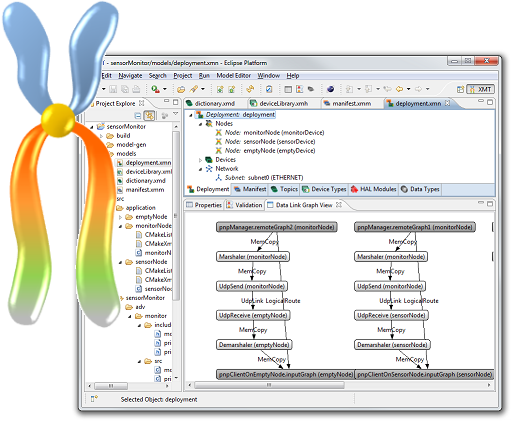
\includegraphics[width=.7\textwidth]{figures/xme_xmt.png}}
\author{%
	fortiss GmbH\\[6pt]
	An-Institut an der\\
	Technischen Universit\"at M\"unchen\\[6pt]
	Guerickestr. 25\\
	80805 M\"unchen\\[6pt]
	\url{chromosome@fortiss.org}
}
\date{Version \xmeVersionNumber{} \xmeVersionSuffixCaps{}\\\xmeVersionDate{}}

\begin{document}
\maketitle

\vfill
\begin{quote}
Copyright (c) 2011-2014, fortiss GmbH.\\
Licensed under the Apache License, Version 2.0.\\[6pt]

Use, modification and distribution are subject to the terms specified
in the accompanying license file LICENSE.txt located at the root directory
of this software distribution. A copy is available at
\url{http://chromosome.fortiss.org/}.\\[6pt]

Trade names, trademarks and registered trademarks are used without special marking throughout the source code and/or documentation.
All are the property of their respective owners.
\end{quote}

\newpage
\tableofcontents
\newpage

%
% Copyright (c) 2011-2013, fortiss GmbH.
% Licensed under the Apache License, Version 2.0.
% 
% Use, modification and distribution are subject to the terms specified
% in the accompanying license file LICENSE.txt located at the root directory
% of this software distribution. A copy is available at
% http://chromosome.fortiss.org/.
%
% This file is part of CHROMOSOME.
%
% $Id: introduction.tex 6238 2013-12-20 16:59:17Z ruiz $
%

\section{Introduction} \label{sec:intro}

For a long time, the focus of embedded systems development has been the implementation of isolated systems with clearly defined boundaries and interfaces.
Recently, the trend of integrating such independent systems into larger \emph{systems of systems} arises.
For example, nodes in a wireless sensor network connect \textit{ad-hoc} to other nodes, manufacturing plants get connected with logistics
and intelligent cars communicate with each other and the infrastructure.
Due to the different life cycles of the involved systems, adaptability such as plug~\&~play becomes more and more important.
Systems must allow integration with each other even if the exact type and structure of their counterparts is not known at design time
without losing their safety, security and real-time capabilities.

In order to achieve this, a powerful domain-independent software platform is required,
which can flexibly be adapted to various application scenarios.
\xme\footnote{\url{http://chromosome.fortiss.org/}} is a middleware and runtime system intended to meet these requirements.
It combines features known from the embedded domain such as determinism with adaptivity known from internet technologies.
\xme treats extra-functional requirements as first-class entity and provides according mechanisms to fulfill such requirements.

\xme has a large set of designated features and is designed to evolve over time.
Its runtime system is completely open source and hence transparent to developers and end users.

\subsection{In this Release}

This release of \xme consists of two main parts:
\begin{enumerate}
	\item The \xme (XME) runtime system with hardware abstraction layer (HAL) and platform support for Linux and Windows.
	\item The \xmt (XMT), an Eclipse-based model-driven design tool with automatic code generation capabilities for static configuration of the target system.
\end{enumerate}
The objective of the current release is to allow users to \emph{model the distributed system} in a graphical way in XMT
and allow the modeled system to evolve at runtime using \emph{plug and play}.

Based on the XMT model, code is generated for every device (node) in the network of the distributed application.
If user-defined components are used, the user then develops the necessary code that is based on the \xme runtime system.
This makes the code portable between the various target platforms.
Finally, the code is compiled using \xme's powerful build system infrastructure that is based on CMake
and transferred to the respective target systems (this is currently still a manual process).
At runtime, new software components may be added to the nodes using plug and play concepts.

The described features are a subset of the features that will be available in future versions.
Appendix~\ref{appx:roadmap} provides an overview of the anticipated feature roadmap and the respective timeframe.

The following tutorial will introduce you to the main concepts of \xme and illustrate them with examples that are easy to understand.
Including installation of required prerequisites, this tutorial will take about two hours to complete.

\clearpage

\subsection{The Name \xme}

\xme stands for \textbf{\underbar{Cro}}ss-domain \textbf{\underbar{M}}odular
\textbf{\underbar{O}}perating \textbf{\underbar{S}}ystem \textbf{\underbar{o}}r
\textbf{\underbar{M}}iddlewar\textbf{\underbar{e}}.\footnote{We borrowed the ``H'' from somewhere else.}
The name expresses the vision of \xme:
\begin{enumerate}
	\item We believe that in the future cross-domain solutions for networked embedded systems are required.
	\item As different applications might have many different requirements
		and the middleware will be deployed to very heterogeneous platforms,
		a scalable and modular solution is required.
	\item \xme will sometimes operate on top of an operating system (OS),
		but it might also replace an OS due to resource constraints.
		We think that in the future, the boundary between an operating system and a middleware will be blurry.
\end{enumerate}

Similar to biology, a \xme instance is built up by a number of genes (here software components).
It is not the intention of \xme to invent new genes, but instead to use
existing protocols/solutions to implement components for specific tasks.
The major idea is that \xme offers a flexible blueprint that enables the
selection of different solutions to adapt a system to the specific requirements.

Analog to the evolution of mankind, we do \emph{not} believe that the genes provided by \xme are initially perfect.
Instead we believe in constant improvement based on discussions about specific components.
This is one of the reasons why we are offering \xme as open-source software.
In case you have any questions or suggestions for improvement, we are looking forward to your comments.

\subsection{Mailing Lists}

We offer two mailing lists for CHROMOSOME-related topics:
\begin{itemize}
	\item \textbf{News and release announcements:} \url{chromosome-announce@lists.fortiss.org} \\
		Archives: \url{https://lists.fortiss.org/pipermail/chromosome-announce/} \\
		To subscribe, send an (empty) e-mail to \url{chromosome-announce-subscribe@lists.fortiss.org}.
		You will then receive an automatic e-mail with further instructions.
		This list is read-only.
	\item \textbf{Developers:} \url{chromosome-dev@lists.fortiss.org} \\
		Archives: \url{https://lists.fortiss.org/pipermail/chromosome-dev/} \\
		To subscribe, send an (empty) e-mail to \url{chromosome-dev-subscribe@lists.fortiss.org}.
		You will then receive an automatic e-mail with further instructions.
		To start a discussion, send an e-mail to \url{chromosome-dev@lists.fortiss.org}.
		You do not need to subscribe in order to be able to post.
		In this case, let other people know that you would like to be \texttt{CC:}'d in replies.
\end{itemize}

\subsection{Questions and Contact Information}

If you have any questions with respect to this tutorial or want to report a bug,
please check the mailing list archives and the Frequently Asked Questions in Appendix~\ref{appx:faq}.
If your question is not answered, please post to the \url{chromosome-dev@lists.fortiss.org} mailing list.

\subsection{Acknowledgments}

This work is partially funded by the following research grants:
\begin{itemize}
	\item German Federal Ministry of Economics and Technology (BMWi) research grant 01ME12009
		(project RACE\footnote{\url{http://www.projekt-race.de/}})
	\item German Federal Ministry of Economics and Technology (BMWi) research grant 01MA11002
		(project AutoPnP\footnote{\url{http://www.autopnp.com/}})
	\item Bavarian Ministry of Economic Affairs, Infrastructure, Transport and Technology grant programme 1330/686
		(Vorlaufforschung fortiss)
\end{itemize}

\clearpage
%
% Copyright (c) 2011-2013, fortiss GmbH.
% Licensed under the Apache License, Version 2.0.
% 
% Use, modification and distribution are subject to the terms specified
% in the accompanying license file LICENSE.txt located at the root directory
% of this software distribution. A copy is available at
% http://chromosome.fortiss.org/.
%
% This file is part of CHROMOSOME.
%
% $Id: prerequisites.tex 6238 2013-12-20 16:59:17Z ruiz $
%
% Author:
%         Dominik Sojer <sojer@fortiss.org>
%         Michael Geisinger <geisinger@fortiss.org>
%

\section{Prerequisites (30 minutes)}
\label{sec:prereq}

\xme has been developed with platform independence in mind.
This tutorial covers both Linux\footnote{%
	When we say Linux, we actually mean the many distributions that are out there.
	\xme has been specifically tested with Debian-like environments such as Ubuntu and Xubuntu.
	However, we believe that there are no fundamental hurdles that would prevent it from running on other Linux distributions.
	The \xme runtime system by default has no GUI and should also run on plain UNIX-based systems, provided enough resources are available.
	For using the \xmt, a graphical desktop environment is required, however.
	If you experience problems, or got it to work on an exotic platform, please let us know!
} and Windows development and target platforms.
%
While installing the proposed build environment, you might want to start reading Section~\ref{sec:architecture} giving an overview on \xme and its features.

\subsection{Prerequisite Installation on Linux}
\label{sec:prereq:linux}

Apart from the \xme source archive, the following packages are recommended for building \xme applications on Linux.
\begin{itemize}
	\item \textbf{GCC Toolchain}:
		GCC offers a complete compiler toolchain for various languages
		and is recommended for compiling C/C++ programs natively on Linux.
		Install it as well as some tools by issuing the following command:\footnote{%
			The \texttt{apt-get} command is specific to Debian-like Linux distributions.
			Use the respective command on other distros.
		}
		
		\verb|sudo apt-get install gcc g++ gdb make|
	
	\item \textbf{CMake} (at least version 2.8.5):
		CMake is a cross-platform Makefile generator and is used to manage the build system.
		Output of CMake are the build system configurations (here UNIX Makefiles or Eclipse CDT projects).
		\xme provides a customized set of macros to deal with components, dependencies, executables and documentation.
		First try whether CMake is available as a package in your distribution:
		
		\verb|sudo apt-get install cmake|
		
		It is also meaningful to install \verb|ccmake|, an \verb|ncurses|-based GUI for CMake:
		
		\verb|sudo apt-get install cmake-curses-gui|
		
		If CMake is not available in your distribution, it is very easy to build and install it from source.
		Download the source package from the Kitware website\footnote{\url{http://www.cmake.org/cmake/resources/software.html}}
		and follow the instructions.
		\xme currently requires at least CMake version 2.8.5.
		If installation worked properly, this command should tell you the installed version of CMake:
		
		\verb|cmake --version|
\end{itemize}
%
The following packages are recommended in addition if you plan to develop applications with \xme.
\begin{itemize}
	\item \textbf{Perl}:
		Various maintenance script and tools use the Perl scripting language.
		Even if not mandatory for \xme, Perl might be worth a look:
		
		\verb|sudo apt-get install perl|
	
	\item \textbf{Doxygen}:
		Doxygen is used to automatically generate source code-level documentation that is meaningful for users of a given API.
		For this purpose, the \xme source files have been annotated with respective comments.
		If your distro offers the \texttt{doxygen} package, all you have to do is:
		
		\verb|sudo apt-get install doxygen|
		
		Otherwise, please download and install manually from the Doxygen website.\footnote{%
			\url{http://doxygen.org/}
		}
	
	\item \textbf{Graphviz}:
		A graph drawing package.
		Doxygen uses this to enhance the generated documentation with inclusion graphs, dependency graphs and class diagrams:
		
		\verb|sudo apt-get install graphviz|
		
		Otherwise, please download and install manually from the Graphviz website.\footnote{%
			\url{http://www.graphviz.org/}
		}
	
	\item \textbf{Expect}:
		Some automation tasks for testing the integrity of our example projects interact dynamically with the respective console programs.
		For this purpose, \verb|expect| is used. Install it as follows:\footnote{%
			This will also install \texttt{tcl}, the Tool Command Language.
			If you've never heard of it, you might want to explore it and its graphical user interface (GUI) addon \texttt{tk}.
			It's great for (GUI) applications that should be nice, platform independent and well scriptable at the same time.
		}
		
		\verb|sudo apt-get install expect|
		
		Otherwise, please download and install manually from the Expect website.\footnote{%
			\url{http://expect.sourceforge.net/}
		}
		
\end{itemize}

\subsection{Prerequisite Installation on Windows}
\label{sec:prereq:windows}

Apart from the \xme source archive, the following tools are required for building \xme applications on Windows.
\begin{itemize}
	\item \textbf{Visual Studio C++} (Express, Professional, Premium or Ultimate, preferably 2008 or 2010 versions):
		Visual Studio is Microsoft's platform for multi-language development.
		The so-called ``Express Edition'' is available free for evaluation purposes.\footnote{%
		\url{http://www.microsoft.com/visualstudio/en-us/products/2010-editions/visual-cpp-express}}
		Note that \xme has not yet been tested with newer versions of Visual Studio than the 2010 release.
		You only have to install the C/C++ compiler. Additional packages like Silverlight or SQL Server are not required.
		Consult Appendix~\ref{appx:install_vs} for details.
		
		In case you want to use a different compiler toolchain, you are welcome to try it out.
		We offer some initial support for building under Cygwin using GCC or MinGW.\footnote{%
			Let us know about your experiences.
			If you prefer using different compilers, we may add them to our portfolio.
		}
	
	\item \textbf{CMake} (at least version 2.8.5):
		CMake is a cross-platform Makefile generator and is used to manage the build system.
		Output of CMake are the build system configurations (here a Microsoft Visual Studio Solution).
		\xme provides a customized set of macros to deal with components, dependencies, executables and documentation.
		CMake can be downloaded for free.\footnote{\url{http://www.cmake.org/cmake/resources/software.html}}
		\xme currently requires at least CMake version 2.8.5.
		It is \emph{not} necessary to add CMake to the system search path.
		Consult Appendix~\ref{appx:install_cmake} for details.
\end{itemize}
%
The following optional tools are recommended in addition if you plan to develop applications with \xme.
\begin{itemize}
	\item \textbf{Cygwin}:
		Cygwin is a UNIX emulation environment that comes with a set of useful tools.
		You can find the download and installation instructions on its website.\footnote{\url{http://www.cygwin.com/}}
		Although the tools are based on an emulation layer, the performance is still acceptable and maintenance is simple.
		The drawback is that the versions offered are typically a little bit outdated.
		In case this is not acceptable, download and install the tools natively from their respective websites.
		It is recommended to explicitly install the following Cygwin packages
		(see respective items in Section~\ref{sec:prereq:linux} for more information):
		
		\verb|perl|, \verb|expect|
	
	\item \textbf{Doxygen}:
		Doxygen is used to automatically generate source code-level documentation that is meaningful for users of a given API.
		For this purpose, the \xme source files have been annotated with respective comments.
		If you choose not to install \verb|doxygen| as a Cygwin package,
		please download and install manually from the Doxygen website.\footnote{%
			\url{http://doxygen.org/}
		}
	
	\item \textbf{Graphviz}:
		A graph drawing package.
		Doxygen uses this to enhance the generated documentation with inclusion graphs, dependency graphs and class diagrams.
		Please download and install manually from the Graphviz website.\footnote{%
			\url{http://www.graphviz.org/}
		}
	
\end{itemize}

\clearpage
%
% Copyright (c) 2011-2013, fortiss GmbH.
% Licensed under the Apache License, Version 2.0.
% 
% Use, modification and distribution are subject to the terms specified
% in the accompanying license file LICENSE.txt located at the root directory
% of this software distribution. A copy is available at
% http://chromosome.fortiss.org/.
%
% This file is part of CHROMOSOME.
%
% $Id: xme_overview.tex 7852 2014-03-14 16:32:01Z geisinger $
%

\section{\xme in a Nutshell (30 minutes)}
\label{sec:architecture}

\xme (often abbreviated by ``XME'') is a domain-independent, data-centric\footnote{%
For details, please refer to \url{http://www.omg.org/news/whitepapers/Intro_To_DDS.pdf}}
middleware for cyber-physical systems.
%
From the point of view of an application component,
\xme abstracts from basic functionality that is traditionally found in operating systems and middlewares,
like scheduling and communication.
Apart from that, it offers model-driven design tools with code generation capabilities
that allow a user to design the distributed system in an abstract way.
%
This section will give the reader a very high level overview of the most important \xme features.
For in-depth information and concrete specifications, the reader is kindly referred to the commented source code of \xme.

\subsection{Goals of \xme}
\xme is designed to match the requirements of future cyber-physical systems.
As a research prototype, the main intention is to serve as a basis
for discussion how future middleware/operating system architectures may look like.
The development is done in a demand-driven way.
Depending on the requirements of projects where \xme is applied, new features in \xme will be introduced.

Our point of view is that
future middleware will not operate on a specific class of devices, but will run on very heterogeneous platforms.
The exaggerated goal statement could be to ``develop a middleware serving a range from 8-bit controllers to cloud servers''.\footnote{%
	This is a very striking motto.
	The functionality offered by the middleware will of course vary depending on the resource constraints of the target platform.
}
%
Hence, scalability and modularity of the middleware is of highest importance. It must be easy to remove or add components from/to 
the middleware. Similar to micro-kernel operating systems, the core of \xme must be very small and only contain the absolutely necessary
features. Since the boundaries of operating systems, middleware, and applications are vanishing, one unique mechanism must be supported to
add components on all these levels.

%\paragraph{Concept 1: Data-Centric Design}
\paragraph{Data-Centric Design}
A very successful concept to achieve scalability is message-orientation as for example demonstrated by the QNX\footnote{\url{http://www.qnx.com/}} neutrino micro-kernel.
However, one major drawback of this concept is the necessity of requiring knowledge of both the sender and the receiver.
In the context of systems-of-systems where the communication partners are not known at design time, message orientation cannot be applied.
Therefore, \xme is based on the very powerful concept of data-centric design. Components specify which data they consume
and produce and depending on this information, the middleware calculates the communication routes.

It is important to note that in contrast to prominent other middleware systems relying on data-centric design,
\xme does not broadcast the data, instead it calculates specific routes based on the requirements.
This allows for a very efficient implementation. Furthermore, the routes are calculated only when components are added or removed. Based
on the experience in embedded systems, we assume that reconfiguration takes place less often than the transmission of data items.
Similar to concepts from multimedia protocols,
our initial assumption is that data transmission has to happen within real-time,
while reconfiguration is not time-critical or has only soft real-time requirements.

Data is grouped by so-called \emph{topics}. A topic is a data type with a certain structure.
Examples for topics are \emph{temperature}, \emph{rotation speed} or \emph{GPS position}. Topics are defined for a specific domain.
This enables the exchange of data between different applications.
%To allow cross-domain communication, we plan to define translation matrixes between the topics of different domains.
%
Topics are organized in so-called \emph{topic dictionaries}.
Each dictionary contains topic definitions for a specific domain and/or application.

%\paragraph{Concept 2: Refinement of Topics with Attributes}
\paragraph{Refinement of Topics with Attributes (partially implemented)}
Exchange of data can only be automated if the requirements on data are specified explicitly.
This includes information about the quality of data such as \emph{age}, \emph{accuracy}, \emph{confidence} and \emph{safety level}.
In the respective topic dictionary, each topic can be annotated with so-called \emph{attributes}.\footnote{Called \emph{meta-data} in previous versions of \xme.}
An attribute consists of a \emph{key} (its name) and its \emph{value}.
Depending on the type of attribute, the concrete value may be constant, known at configuration time or dynamically calculated during runtime.
%\TODO{[REWORK]
%\begin{itemize}
	%\item \textbf{Static meta-data:}
		%Application components have fixed requirements and guarantees.
		%Meta-data are used to calculate the appropriate communication routes at configuration time.
		%For example, imagine a temperature sensor network for building automation.
		%Depending on its size, multiple sensors may be present in a room.
		%Each sensor would specify its \emph{location} as meta-data.
		%A climate control component that controls the air conditioning system for a specific room would specify, using meta-data,
		%that it only wants to receive temperature data from sensors that match the respective room.
	%
	%\item \textbf{Dynamic meta-data:}
		%Application components producing data may specify meta-data such as the quality of the transmitted values dynamically during runtime.
		%Consuming components may have dynamic meta-data acceptance filters and may use meta-data also for their calculations.
		%For example, imagine that one of the rooms in the auotmated building from the previous example is a server room.
		%In this case, a high reliability is required.
		%Using meta-data about the confidence of each sensor,
		%the climate control may dynamically calculate the confidence in its own set value for the air conditioning system.
		%The association of data from the respective room could still use static meta-data.
%\end{itemize}
%}
%
Using attributes, application components describe their requirements respectively guarantees on data.
This information can be used to select appropriate communication streams while still retaining independence between sender and receiver.

%\paragraph{Concept 3: Data Access}
%Components can access data in two different ways. As standard operation, \xme provides a publish-subscribe mechanism. Each component states
%which data is required and which data is produced. The middleware ensures the routing of the specific data. If data is only required 
%seldomly in comparison to the data production rate, a request-response mechanism is offered to the application developer.

%\paragraph{Concept 4: Timing (not yet implemented)}
\paragraph{Model of Execution (partially implemented)}
Correct timing is a major concern for cyber-physical systems.
\xme abstracts the concrete implementation, but currently offers mechanisms to specify schedules for time-triggered execution.
In future versions, end-to-end-timing and jitter requirements for data paths will also be supported.

The reason to abstract the concrete implementation/concrete configuration
in \xme is on the one hand to reduce the development effort by automatically deriving a concrete configuration satisfying the timing
requirements (if a configuration exists) and on the other hand to support plug~\&~play capability. The state of the art in embedded system
design requires the developer to configure the application in a correct way. Several configurations might be valid, but typically only one
configuration is specified. It is not possible for the run-time system to change the configuration, as the real requirements are not present
any more and the system can not calculate alternative configurations. By explicitly stating the requirements and leaving configuration issues
to the run-time system, this problem can be avoided.
The system can support new components by calculating a new configuration that satisfies both
the requirements of already running applications and the newly installed applications.

It is important to note that \xme can of course only offer guarantees that are enabled by the underlying platform.
In case \xme runs on a Linux or Windows system without real-time kernel/extensions,
\xme will not be able to satisfy jitter requirements in the range of microseconds.
Nevertheless, certain implementations on top of such systems may offer very good guarantees.
The major concept here is to use algorithms that offer determinism sacrificing average-case performance.
Examples are the implementation of a time-triggered communication scheme on top of Ethernet.
This implementation guarantees collision free communication, but comes with a lower bandwidth and flexibility.

%\paragraph{Concept 5: Resource-Awareness (not yet implemented)}
%\xme is designed to be able to handle all resources of the platform.
%The major idea is that components/applications can state their worst-case resource requirements
%on memory, computation time, bandwidth, etc.
%\xme will then ensure that enough resources are available to allow the execution of this component/application.
%
%\paragraph{Concept 6: Other extra-functional properties -- Fault-tolerance, QoS, Security (not yet implemented)}
%\xme is designed in a way such that components which guarantee other extra-functional properties can be easily extended.
%Examples on extra-functional properties that are currently being integrated in \xme are fault-tolerance, QoS, and security.
%
%\paragraph{Concept 7: Support for States (not yet implemented)}
%A very important topic to ensure resource efficiency is state awareness.
%We are currently thinking about possibilities to support states
%(each one with a set of active applications) in \xme.
%The support of (sub-)system wide states would simplify the development of applications,
%but also other aspects such as fault-tolerance.

\paragraph{Plug \& Play}

One of \xme's major goals is to allow dynamic reconfiguration of a distributed application at runtime.
In order to combine this concept with real-time capabilities and determinism, we distinguish between the so-called \emph{plug phase} and the \emph{play phase}.
The plug phase, which is entered upon startup and can on demand be triggered during runtime,
is used to analyze the requirements of all components and to develop a plan for configuring the runtime system in order to meet the dependencies.
The plug phase is not real-time capable, i.e., its exact duration is not guaranteed.
During the plug phase, component requirements are checked, binaries are copied, data paths are calculated and the configurations for every element in the system are prepared and deployed.
For this purpose, plug \& play related components on all nodes in the network cooperate.

When the configuration is finished, the system transitions to the play phase.
The play phase is deterministic with respect to the requirements stated by the components, such as the worst-case execution time.

Subsequent plug \& play events may be triggered in the play phase,
for example node plugout (i.e., the removal of nodes from the XME ecosystem)
or removal of individual components.

\paragraph{Health Monitoring (partially implemented)}

Although the system is deterministic during the play phase, a runtime health monitoring is required,
because an application component might violate its asserted requirements.
For example, an application component might violate its worst-case execution time or try to access a resource where it has no access to.
Similarly, a network communication problem might occur.
In such cases, the system is supposed to fall back into a safe mode in which the basic functionality of the application is retained.
This allows for safe ``shutdown''.

\subsection{Glossary}
\label{sec:architecture:glossary}

This glossary explains the most important terms in \xme in alphabetical order.

\paragraph{Component}
A component is a modular software unit that has input and output interfaces, so-called \emph{ports}.
A component consist of at least one \emph{function}.

\paragraph{Component Wrapper}
A component wrapper is the interface between a component and the \emph{Data Handler} core component.
For every input port of the respective component, it offers a respective reading function.
For every output port of the respective component, it offers a respective writing function.
The reading and writing functions are called by the component's functions.
The component wrapper enforces the isolation between \xme core components and (untrusted) functions with respect to data passing.

\paragraph{Ecosystem}
A collection of \xme nodes that communicate with each other.
Nodes can be added to and removed from an \xme ecosystem via plug \& play.

\paragraph{Function}
A function is a primitive algorithm that is associated with a \emph{component}.
It may read a subset of its \emph{component}'s input \emph{ports} and may write a subset of its \emph{component}'s output ports.
Functions are annotated with their worst-case execution time.

\paragraph{Function Wrapper}
The function wrapper is the interface between the \emph{Execution Manager} component and a function.
Whenever the \emph{Execution Manager} runs a function, it does not directly call the function,
but instead it unblocks the thread that executes the respective function wrapper.
The function wrapper then ensures that all data that the respective function needs are readily available and then calls the function.
When the function returns, the function wrapper signals the \emph{Execution Manager} accordingly.
The function wrapper enforces the isolation between \xme core components and (untrusted) functions with respect to execution.

\paragraph{Node}
In terms of \xme, a node is an instance of the \xme runtime system that implements a certain part of a (possibly distributed) application.

\paragraph{Node Identifier}
A node identifier is a number uniquely identifying a \emph{node} in a \xme network.
Node identifiers are maintained by the \emph{Login Manager}.

\paragraph{Play Phase}
Time where the distributed system is running in order to achieve the intended task.
Opposite of \emph{plug phase}.

\paragraph{Plug Phase}
Time where the distributed system is being configured or reconfigured automatically, depending on specified requirements.
Plug phase is entered on system startup or on request by the user or \emph{Plug \& Play Manager}.
Opposite of \emph{play phase}.

\paragraph{Port}
A port is an input or output interface of a component.
Ports are associated with a specific \emph{topic} that defines the type of data expected respectively emitted by the port.
Ports may be implemented by a single memory cell, a queue, or a ring buffer, for example.
A port specifies whether it is persistent, that is whether the last received value contained in a port will be kept around for further read operations or not.

\paragraph{Topic}
A topic is a type of data transmitted between \emph{ports} of \emph{components}.

\paragraph{Waypoint}
A waypoint is a lightweight component that applies a certain transformation to data.
For example, marshaling and demarshaling are two waypoints.
Likewise, sending and receiving of data according to a specific protocol are represented by two waypoints.\footnote{%
	In previous versions of \xme, the now obsolete \emph{Interface Manager} was responsible for transferring data over the network.
}
Waypoints have a configuration interface which is used to ``program'' their tasks during \emph{plug phase}.
During \emph{play phase}, waypoints deterministically achieve their task according to their configuration.

\begin{figure}[htb]
	\centering
	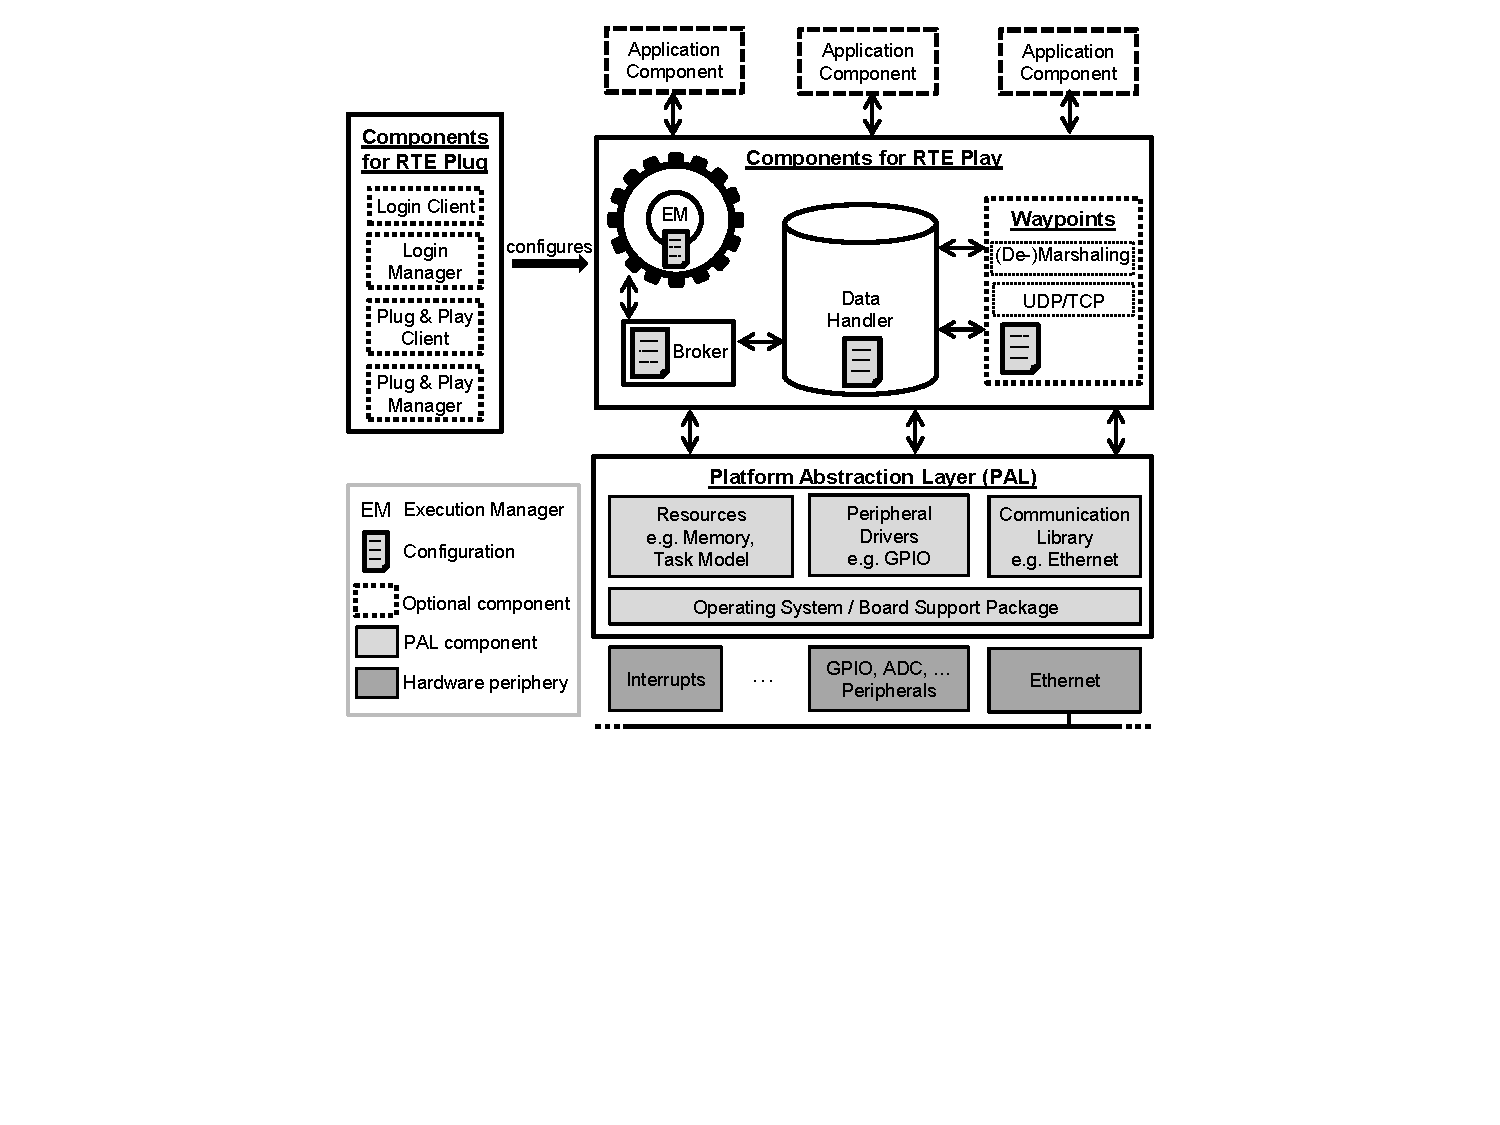
\includegraphics[width=0.8\textwidth,trim=166 190 166 5]{figures/architecture.pdf}
	\caption{\xme architecture overview.}
	\label{fig:architecture}
\end{figure}



\subsection{\xme Components}

\label{sec:core_components}
\xme is designed in a modular fashion. Its component-oriented architecture is depicted in Figure~\ref{fig:architecture}.
A (distributed) \emph{application} consists of a set of (software) \emph{components} that interact with each other by exchanging data.
Each component is placed on a specific \emph{node} in the network.
On operating system based platforms like Linux or Windows,
the software of a node is typically represented by a console application.
On embedded systems, the software of a node corresponds to the firmware.
A component may contain a number of \emph{functions} that exchange data via the \emph{ports} of their parent component.
A component's \emph{input port} may receive data from other components and forward it to one of its functions for processing.
Functions may generate data for publication on their parent component's \emph{output ports}.

The following sections provide brief descriptions of the most important components of \xme.
See Figure~\ref{fig:architecture} for a graphical illustration.



\subsubsection{Mandatory Components for RTE Play}

``RTE play'' refers to the normal execution of a \xme node.

\paragraph{Broker}
The Broker ``knows'' which function depends on which data in the input ports of their parent components.
As such, it knows when a function has enough data to be executed.
When data is available on an output \emph{port} of a \emph{component}, the Broker copies them to the dependent input \emph{ports} by triggering a transfer function in the \emph{Data Handler}.
Hence, the Broker offers an interface where the \emph{Execution Manager} can query whether a function is currently ready for execution.\footnote{%
	In previous versions of \xme, the Broker was responsible for delivering data to components.
	In this version of \xme, the actual transfer is achieved by the \emph{Data Handler}.
}

\paragraph{Execution Manager}
The Execution Manager is responsible for executing functions that are ready for execution.
Depending on the model of execution (currently, only time triggered execution is supported),
the Execution Manager has a set of schedules (time triggered) or priorities (event triggered), or both (hybrid).

In the time triggered case, the Execution Manager executes checks for every component
whether it is ready for execution in a round-robin fashion.
For this purpose, it asks the \emph{Broker} whether the data dependencies of the respective function are satisfied.
Under all functions that are ready for execution, the Execution Manager chooses one to execute.
While a function is executed, it reads data from the ports of the respective component (by calling respective functions in the \emph{Data Handler}).
This may lead to the function not being executable any more in the next cycle.

\paragraph{Data Handler}

The Data Handler offers a central storage for all data exchanged via data centric communication ports of components on a node.
The \emph{component wrappers} interact with the Data Handler by reading and writing data and attributes.



\subsubsection{Optional Components for RTE Plug}

``RTE plug'' refers to reconfigurability aspects of \xme.

\paragraph{Logical Route Manager}
The Logical Route Manager (not shown in Figure~\ref{fig:architecture})
receives a list of all publications and subscriptions from the \emph{Plug \& Play Manager}
when the system configuration is to be updated (\emph{plug phase}).
Based on this information, the Logical Route Manager calculates logical routes,
i.e., it finds sources and sinks with matching topics and attributes.
The set of logical routes is forwarded to the \emph{Network Configuration Calculator}.

\paragraph{Network Configuration Calculator}
The Network Configuration Calculator (not shown in Figure~\ref{fig:architecture}) takes the logical routes calculated by the \emph{Logical Route Manager}
and enhances them with communication protocol specific transformation steps that are applied to the data
in between the sender (publication) and the receiver (subscription).
We call such transformations \emph{waypoints} on the data path.
Furthermore, the Network Configuration Calculator calculates where in the network the individual waypoints are to be placed.
The result is a set of physical routes and deployment information that is sent back to the \emph{Plug \& Play Manager}.

\paragraph{Plug \& Play Manager}
The Plug \& Play Manager is responsible for handling requests for dynamic changes to the running system.
It is also responsible for the startup procedure.
The Plug \& Play Manager is either triggered by a system reset, by the user, or by the login or logout of a node in the network.
It calculates the set of changes that will be applied to the system and triggers other components accordingly,
such as the \emph{Logical Route Manager}, the \emph{Network Configuration Calculator}, or the \emph{Plug \& Play Clients} on remote nodes.
Only one Plug \& Play Manager should exist in a network.

\paragraph{Plug \& Play Client}
The Plug \& Play Client (not shown in Figure~\ref{fig:architecture}) receives commands from the \emph{Plug \& Play Manager} that is present on a specific node in the network.
It interprets those commands and adapts the configuration of local components accordingly, such as the \emph{Broker}, the \emph{Data Handler}, and the \emph{Execution Manager}.

\paragraph{Login Client}
The Login Client (not shown in Figure~\ref{fig:architecture}) is responsible for connecting a node
to other nodes in the network and obtaining a so-called \emph{node identifier}.
The node identifier is a unique address of the node within a network.
The Node Manager periodically tries to obtain such a node identifier from the \emph{Login Manager},
which is present on one specific node in the network.
%
This component is optional, because in statically configured networks, no login or logout might be necessary or supported.

\paragraph{Login Manager}
The Login Manager receives login requests from the \emph{Login Client}s of all other nodes and handles them by assigning respective \emph{node identifiers}.
Only one Login Manager should exist in a network.

\paragraph{Node Manager}
A node can have an arbitrary amount of software components that implement the application.
The Node Manager (not shown in Figure~\ref{fig:architecture}) provides management mechanisms for managing existing components and instantiating new components.



\subsubsection{Primitive Components}

Primitive Components directly access the \emph{Hardware Abstraction Layer} using function calls
and offer data obtained from the hardware in a data centric way or forward data to the respective actuators.
They are typically the source of physical data obtained from the environment and
the sink for control data to the environment.



\subsubsection{Platform/Hardware Abstraction Layer}

The Platform/Hardware Abstraction Layer, often abbreviated by PAL or HAL,
provides a platform independent application programming interface (API).
\xme \emph{components} are usually implemented against that API and are hence platform independent.
The HAL implements hardware-specific functionality such as drivers for microcontroller periphery
like general purpose I/O (GPIO) or analog to digital conversion (ADC),
but it also provides a lot of software functions similar to an operating system.
See the content of the directory \verb|<XME_ROOT>/xme/hal/include|\footnote{%
	\texttt{<XME\_ROOT>} specifies the root of the \xme source package.
	See Chapter~\ref{sec:example_sensorMonitor} for details.
}
for an overview of the supported functionality.
Each header file in this directory corresponds to a HAL module
and contains documentation about the provided functionality.

\subsubsection{Application Components}

The actual (distributed) application running in the network is implemented by specific Application Components.
They typically operate only on data obtained via data centric communication.
In particular, no direct access to the Hardware Abstraction Layer with effects in the environment should be made,
instead Application Components should use \emph{Primitive Components}.
This design concept leads to modular, reusable components.



%\subsubsection{IP Login Client Proxy and IP Login Manager Proxy}
%
%These components are required for new nodes to initially contact the Login Manager.
%A node that does not have a Login Manager will usually have a \emph{Login Manager Proxy} component for each of its physical network interfaces.
%These components are named according to their associated interface types,
%for example \emph{IP Login Manager Proxy} for an Ethernet interface with IP communication stack.
%Whenever the Node Manager, which is responsible for periodic login requests, issues a login request,
%the Login Manager Proxy takes care of broadcasting it over its associated communication interface.
%
%Nodes that have a Login Manager component usually also have a \emph{Login Client Proxy} for each of their interfaces.
%The Login Client Proxy will receive the login requests issued by the Login Manager Proxy on the respective medium
%and forward them locally to the Login Manager.
%The login response is forwarded in a similar manner.
%%
%This concept makes it possible to separate the login and address assignment logic from specific interface types and communication protocols
%and enables a fine-grained assignment of functionality to each communication interface.



%\subsection{Component Definition and Lifecycle}
%\label{sec:component_definition}
%
%\xme \emph{components} are assigned to one of the following categories according to their ``layer'' within the system:
%\verb|adv| (advanced), \verb|prim| (primitive), \verb|core| (runtime system), \verb|wp| (\emph{waypoint}) or \verb|hal| (hardware abstraction).
%Depending on the category, different mechanisms exist for a component to interact with its environment.
%
%A \xme component is defined by four functions to \emph{create}, \emph{activate}, \emph{deactivate} and \emph{destroy} it,
%illustrated here for a component called \verb|xme_adv_myComponent|:
%\begin{quote}
	%%\verb|xme_core_status_t|\\
	%\verb|xme_adv_myComponent_create(xme_adv_myComponent_configStruct_t*);|\\
	%%\verb|xme_core_status_t|\\
	%\verb|xme_adv_myComponent_activate(xme_adv_myComponent_configStruct_t*);|\\
	%%\verb|void|\\
	%\verb|xme_adv_myComponent_deactivate(xme_adv_myComponent_configStruct_t*);|\\
	%%\verb|void|\\
	%\verb|xme_adv_myComponent_destroy(xme_adv_myComponent_configStruct_t*);|
%\end{quote}
%%
%The distinction between creation/activation and deactivation/destruction is required in case a component needs to be migrated:
%in this case, the component is first deactivated (to obtain a consistent state), then moved and activated at the new location.
%All four functions take a pointer to a configuration structure, which represents the state of the respective component instance.
%Multiple component instances of the same component type usually have their own configuration structures.
%
%A typical task during creation of a component is registration of data demand and data production.
%Furthermore, a component may create (periodic) tasks to implement its functionality.
%These two concepts are illustrated in the following sections.
%
%\subsection{Component Instantiation}
%
%Components can be instantiated by adding them to the so-called \emph{component list}, usually defined in the main program file.
%Mandatory core components (compare Figure~\ref{fig:architecture}) are implicitly added to the list.
%An initial configuration may be provided for each component.
%Listing~\ref{lst:component_list} shows a sample component list with respective configurations.
%
%\begin{lstlisting}[numbers=left,float=htpb,label=lst:component_list,caption=Sample component list with component configurations.]
%/*****************************************************************************/
%/***   Component configurations                                            ***/
%/*****************************************************************************/
%XME_COMPONENT_CONFIG_INSTANCE(xme_core_nodeManager) = ~\label{lst:component_list.initialized_config_begin}~
%{
	%0x00000000021041A1, // deviceType
	%XME_CORE_DEVICE_GUID_RANDOM // deviceGuid
%}; ~\label{lst:component_list.initialized_config_end}~
%
%XME_COMPONENT_CONFIG_INSTANCE(xme_prim_ipLoginServerProxy, 1); ~\label{lst:component_list.uninitialized_config}~
%
%/*****************************************************************************/
%/***   Component descriptor                                                ***/
%/*****************************************************************************/
%XME_COMPONENT_LIST_BEGIN
	%XME_COMPONENT_LIST_ITEM(xme_core_nodeManager, 0) ~\label{lst:component_list.stateful_1}~
	%XME_COMPONENT_LIST_ITEM(xme_prim_ipLoginServerProxy, 0) ~\label{lst:component_list.stateful_2}~
	%XME_COMPONENT_LIST_ITEM_NO_CONFIG(xme_adv_myComponent) ~\label{lst:component_list.stateless}~
%XME_COMPONENT_LIST_END;
%\end{lstlisting}
%
%This example declares that three components (besides internal core components),
%namely \verb|xme_core_nodeManager|, \verb|xme_prim_ipLoginServerProxy| and \verb|xme_adv_myComponent|,
%will be present on this node.
%We can distinguish between the following types of components:
%\begin{enumerate}
	%\item \textbf{Components with internal state:}
		%The \verb|XME_COMPONENT_LIST_ITEM()| macro is used to declare such a component
		%(compare lines~\ref{lst:component_list.stateful_1} and~\ref{lst:component_list.stateful_2}).
		%The second parameter of the macro is the zero-based index of the respective configuration
		%(defined above the list) that is used to initialize the component.
		%
		%Some components expect some of their configuration variables to be initialized properly.
		%For example, the \emph{Node Manager} expects its \emph{device type} and \emph{device GUID}
		%members to be set up.
		%This is achived by assigning values to the respective members
		%when declaring the configuration structure with the \verb|XME_COMPONENT_CONFIG_INSTANCE| macro
		%(compare lines~\ref{lst:component_list.initialized_config_begin}--\ref{lst:component_list.initialized_config_end}).
		%Configurations for multiple components of the same type can be declared
		%by separating multiple initialization blocks with commas and using the respective index in the
		%\verb|XME_COMPONENT_LIST_ITEM()| macro.
		%
		%Other components, like the \emph{IP Login Manager Proxy}, do not require any special configuration.
		%They only need a properly defined configuration structure to store their state during runtime.
		%Again, the \verb|XME_COMPONENT_CONFIG_INSTANCE| macro is used
		%with the second parameter set to the number of configuration structures for that component type to create
		%(we could also declare multiple components of the same type), in this case one
		%(line~\ref{lst:component_list.uninitialized_config}).
	%
	%\item \textbf{Components without internal state:}
		%The \verb|XME_COMPONENT_LIST_ITEM_NO_CONFIG()| macro is used to declare such a component
		%(compare line~\ref{lst:component_list.stateless}).
		%In this case, \verb|NULL| will be passed in the \verb|config| parameters of the four functions introduced in Section~\ref{sec:component_definition}.
%\end{enumerate}
%
%The list item macro calls have to be embedded between the \verb|XME_COMPONENT_LIST_BEGIN| and \verb|XME_COMPONENT_LIST_END| macro calls.
%%
%Components declared in this list are automatically created and activated during startup
%and deactivated and destroyed during shutdown.
%
%\subsection{Sending and Receiving Data}
%
%Before sending data, a component states its intent to the runtime system.
%This is necessary to allow the appropriate communication routes to be set up
%and is usually performed from within a component's \emph{create} function.
%%
%For using data centric communication, \verb|#include| the file \verb|"xme/core/dcc.h"|.
%%
%To inform \xme that a component intends to send data under a specific \verb|topic|, call:
%\begin{quote}
	%\verb|publicationHandle =|\\
	%\verb|    xme_core_dcc_publishTopic(|\\
	%\verb|        topic, XME_CORE_MD_EMPTY_META_DATA, NULL|\\
	%\verb|    );|
%\end{quote}
%
%The actual sending of \verb|data| is performed with:
%\begin{quote}
	%\verb|xme_core_dcc_sendTopicData(|\\
	%\verb|    publicationHandle, &data, sizeof(data)|\\
	%\verb|);|
%\end{quote}
%
%A component can subscribe to a certain \verb|topic| with a given \verb|receiveTopicCallback| function by calling:
%\begin{quote}
	%\verb|subscriptionHandle =|\\
	%\verb|    xme_core_dcc_subscribeTopic(|\\
	%\verb|        topic, XME_CORE_MD_EMPTY_META_DATA, receiveTopicCallback, NULL|\\
	%\verb|    );|
%\end{quote}
%Whenever data matching the given topic is received, the given callback function is invoked.
%The last parameter of the function can be used to pass user-defined data to the callback function,
%for example a pointer to the component's configuration structure.
%%
%\verb|receiveTopicCallback| must have a signature matching \verb|xme_core_dcc_receiveTopicCallback_t|, namely:
%\begin{quote}
	%\verb|void receiveTopicCallback(xme_hal_sharedPtr_t dataHandle, void* userData);|
%\end{quote}
%\verb|dataHandle| is a reference to the memory where the received data is located.
%
%\subsection{Working with Tasks}
%
%Tasks are allocated via the resource manager,
%hence \verb|#include| \verb|"xme/core/resourceManager.h"| to use them.
%A component can create one or multiple asynchronous tasks by calling
%
%\begin{quote}
	%\verb|taskHandle = |\\
	%\verb|    xme_core_resourceManager_scheduleTask(|\\
	%\verb|        startMs, periodMs, XME_HAL_SCHED_PRIORITY_NORMAL,|\\
	%\verb|        taskCallback, NULL|\\
	%\verb|    );|
%\end{quote}
%
%This function registers the \verb|taskCallback| function to be scheduled for execution
%according to \verb|startMs| (number of milliseconds before first invocation) and
%\verb|periodMs| (interval between invocations).
%%
%The last parameter of the function can be used to pass user-defined data to the callback function,
%for example a pointer to the component's configuration structure.
%%
%\verb|taskCallback| must have a signature matching \verb|xme_hal_sched_taskCallback_t|, namely:
%\begin{quote}
	%\verb|void taskCallback(void* userData);|
%\end{quote}
%
%A task can be suspended or resumed by calling:
%
%\begin{quote}
	%\verb|xme_hal_sched_setTaskExecutionState(|\\
	%\verb|    taskHandle, <flag>|\\
	%\verb|);|
%\end{quote}
%
%\verb|<flag>| is a Boolean flag that indicates the new task execution state.
%The call will block until the new state can be enforced,
%which is not the case while the task's callback function is executed.
%%A task's callback function should return periodically
%%and the \verb|periodMs| argument in the \verb|xme_core_resourceManager_scheduleTask()| call
%%should be used to reschedule themselves at the appropriate points in time.
%%
%A task can be aborted by calling:
%
%\begin{quote}
	%\verb|xme_core_resourceManager_killTask(|\\
	%\verb|    taskHandle|\\
	%\verb|);|
%\end{quote}
%
%If this function is called from the task to kill itself, then it will mark the task for deletion and return immediately.
%If it is called from a different task, the function blocks until the task has been removed.
%Similarly to suspension and resuming, a task is not removed until its callback function has returned.

\clearpage
%
% Copyright (c) 2011-2013, fortiss GmbH.
% Licensed under the Apache License, Version 2.0.
% 
% Use, modification and distribution are subject to the terms specified
% in the accompanying license file LICENSE.txt located at the root directory
% of this software distribution. A copy is available at
% http://chromosome.fortiss.org/.
%
% This file is part of CHROMOSOME.
%
% $Id: example_helloworld.tex 7852 2014-03-14 16:32:01Z geisinger $
%

\section{Example 1: Sensor and Monitor (20 minutes)}
\label{sec:example_sensorMonitor}

We will start by compiling a simple application which is used to collect data from the workstation the application is running on,
such as the free space on a certain partition.
We will then extend the example subsequently in later chapters.

Two steps are required to build an application based on \xme:
first, the build system needs to be generated using CMake
and second the application needs to be compiled using the generated build system.
%In \xme, a different build system tree is generated for every single target node in the network.
%This tutorial will only present how CMake can be used to generate the build system for a Windows-based host system.
%
After the installation of the required prerequisites (see Section~\ref{sec:prereq}), the following steps are required:

\subsection{Configuration on Linux}
\label{sec:example_sensorMonitor:linux}

\begin{enumerate}
	\item Download the source archive of \xme from the website \\
		\url{http://chromosome.fortiss.org/}.
	
	\item Extract the archive to a directory of your choice. Either use a GUI tool or type the following commands in the console:
		
		\texttt{user@host:~> tar -xvzf xme-\xmeVersionNumber{}\xmeVersionSuffix{}-src.tar.gz} \\
		\texttt{user@host:~> cd xme-\xmeVersionNumber{}\xmeVersionSuffix{}-src} \\
		\texttt{user@host:~/xme-\xmeVersionNumber{}\xmeVersionSuffix{}-src> ls} \\
		\verb|AUTHORS.txt  examples  INSTALL.txt  README.txt  THIRDPARTY.txt  VERSION.txt| \\
		\verb|doc          external  LICENSE.txt  tests       tools           xme|
	
		The \texttt{xme-\xmeVersionNumber{}\xmeVersionSuffix{}-src} directory contains \verb|LICENSE.txt|.
		From now on, we will call that directory \verb|<XME_ROOT>|.
	
	\item We will now generate the required build system for building an example node.
		For this purpose, we first create a build directory and then run CMake.
		
		\verb|user@host:XME_ROOT> mkdir -p examples/sensorMonitor/build/sensorNode| \\
		\verb|user@host:XME_ROOT> cd examples/sensorMonitor/build|
		
		From now on, we will call that directory \verb|<BUILD_ROOT>|.
	
	\item The example that we are going to build consists of two nodes.
		Create a subdirectory in \verb|BUILD_ROOT| for the first node:
		
		\verb|user@host:BUILD_ROOT> mkdir sensorNode| \\
		\verb|user@host:BUILD_ROOT> cd sensorNode|
	
	\item Generate the required build system for building the sensor node:
		
		\verb|user@host:BUILD_ROOT/sensorNode> cmake -G "Unix Makefiles" \ | \\
		\verb|                                 ../../src/application/sensorNode|
	
	\item Compile the example:
		
		\verb|user@host:BUILD_ROOT/sensorNode> make|
	
	\item Run the example application:
		
		\verb|user@host:BUILD_ROOT/sensorNode> target/sensorNode|
	
	\item Continue in Section~\ref{sec:example_sensorMonitor:common}.
\end{enumerate}

\subsection{Configuration on Windows}
\label{sec:example_sensorMonitor:windows}

\begin{enumerate}
	\item Download the source archive of \xme from the website \\
		\url{http://chromosome.fortiss.org/}.
	
	\item Extract the archive to a directory of your choice.\footnote{%
		On Windows systems, please ensure that the path name is not extraordinary long, as this could cause issues with the build system (depending on the file system used).}
		After extraction you should see a directory that contains \verb|LICENSE.txt|.
		From now on, we will call that directory \verb|<XME_ROOT>|.
		%The subdirectory \verb|bin| contains binaries shipped with the release.
		%This allows testing of \xme without compiling your own applications.

	\item Use the \emph{start menu} to run \emph{CMake (cmake-gui)} (compare Figure~\ref{fig:cmake_run}).
\begin{figure}[htpb]
	\centering
	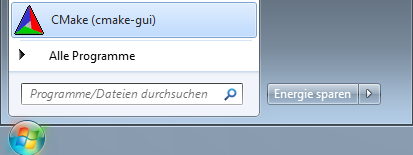
\includegraphics[scale=0.75]{figures/cmake_run.png}
	\caption{\emph{CMake (cmake-gui)} icon in the start menu.}
	\label{fig:cmake_run}
\end{figure}
	\item In the \emph{Where is the source code} field, select the full path to the directory
		\verb|<XME_ROOT>/| \verb|examples/sensorMonitor/src/application/sensorNode| (compare Figure~\ref{fig:cmake_configuration1}).


\begin{figure}[htpb]
	\centering
	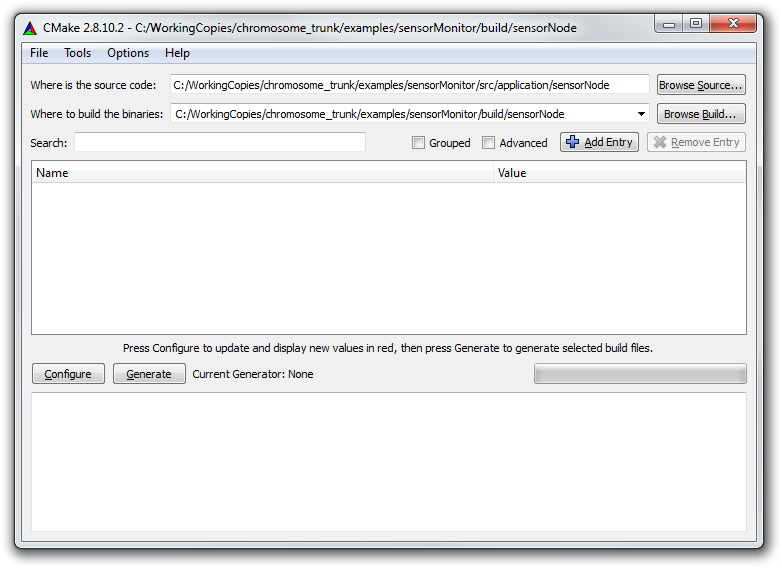
\includegraphics[scale=0.75]{figures/cmake_configuration1.png}
	\caption{Source code and build directory specification.}
	\label{fig:cmake_configuration1}
\end{figure}

	\item In the \emph{Where to build the binaries} field, select the full path to the directory
		\verb|<XME_ROOT>/| \verb|examples/sensorMonitor/build/sensorNode| (note the additional \verb|sensorNode| folder,
		this folder does not yet exist).%\footnote{%
		%This will cause CMake to generate a so-called out-of-source build system, which is recommended.}
	\item Click the \emph{Configure} button.
	\item If asked whether the build directory should be automatically created, say \emph{Yes}.
	\item Choose the \emph{Visual Studio} toolchain that corresponds to your Visual Studio version
		(do \emph{not} use the 64 bit version, even on a 64 bit system) and click \emph{Finish} (compare Figure~\ref{fig:cmake_toolchain}).

\begin{figure}[htpb]
	\centering
	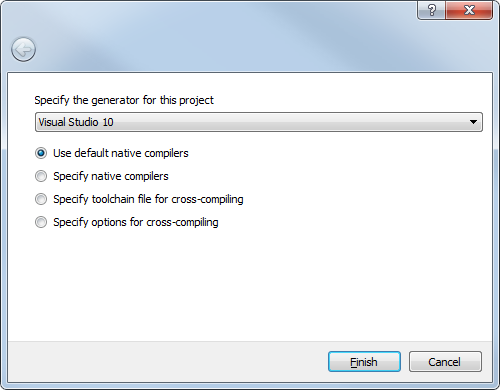
\includegraphics[scale=0.75]{figures/cmake_toolchain.png}
	\caption{Toolchain selection in CMake.}
	\label{fig:cmake_toolchain}
\end{figure}

	\item After CMake has finished its configuration, various configuration variables marked in red should appear in the list
		(compare Figure~\ref{fig:cmake_configuration2}).
	\item Click the \emph{Generate} button.
		This will generate the Visual Studio solution file, called \verb|sensorNode.sln| which you can open in Visual Studio.
		The file will be placed in the following directory: \verb|<XME_ROOT>/examples/sensorMonitor/build/sensorNode| (compare Figure~\ref{fig:build_directory}).

\begin{figure}[h!t]
	\centering
	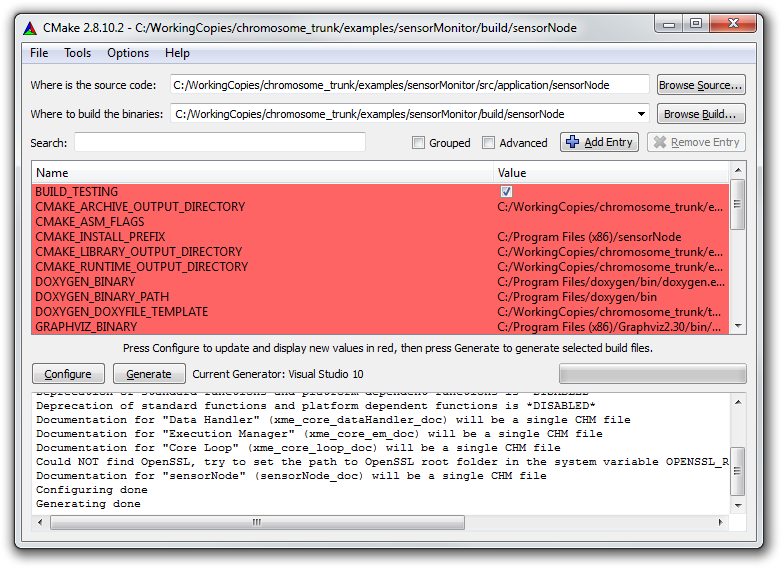
\includegraphics[scale=0.75]{figures/cmake_configuration2.png}
	\caption{Configuration and build system generation in CMake.}
	\label{fig:cmake_configuration2}
\end{figure}

\begin{figure}[htpb]
	\centering
	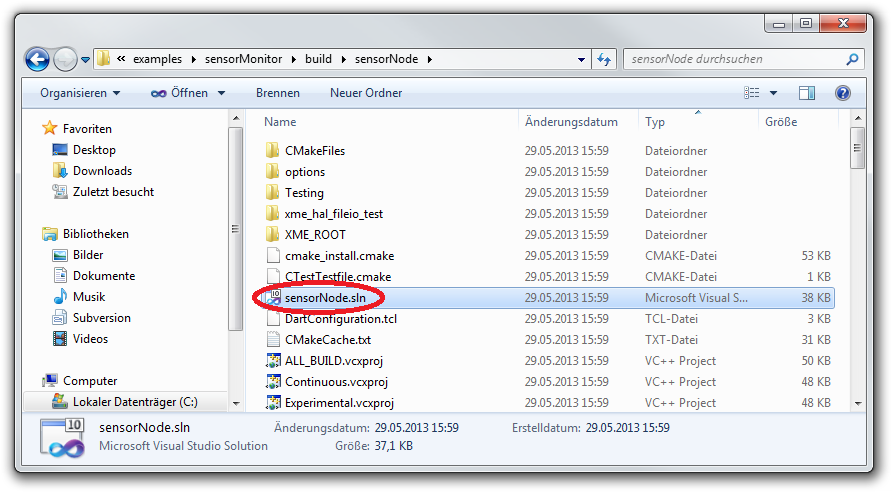
\includegraphics[width=\textwidth]{figures/build_directory_edited.png}
	\caption{Build directory after build system generation, highlighted in red the Visual Studio solution file.}
	\label{fig:build_directory}
\end{figure}

\end{enumerate}

\noindent To compile the exemplified application, the following steps are required:

\begin{enumerate}
	\item Fire up Visual Studio and select \emph{File} $\rightarrow$ \emph{Open} $\rightarrow$ \emph{Project/Solution...}
	\item Navigate to the \verb|<XME_ROOT>/examples/sensorMonitor/build/sensorNode| directory and select the solution file \verb|sensorNode.sln|.
	\item After loading the solution, you will see a project tree in the left-hand pane.
		Right-click on the \verb|sensorNode| project and choose \emph{Set as StartUp Project}
		(compare Figure~\ref{fig:vs_set_as_startup_project}).

\begin{figure}[htpb]
	\centering
	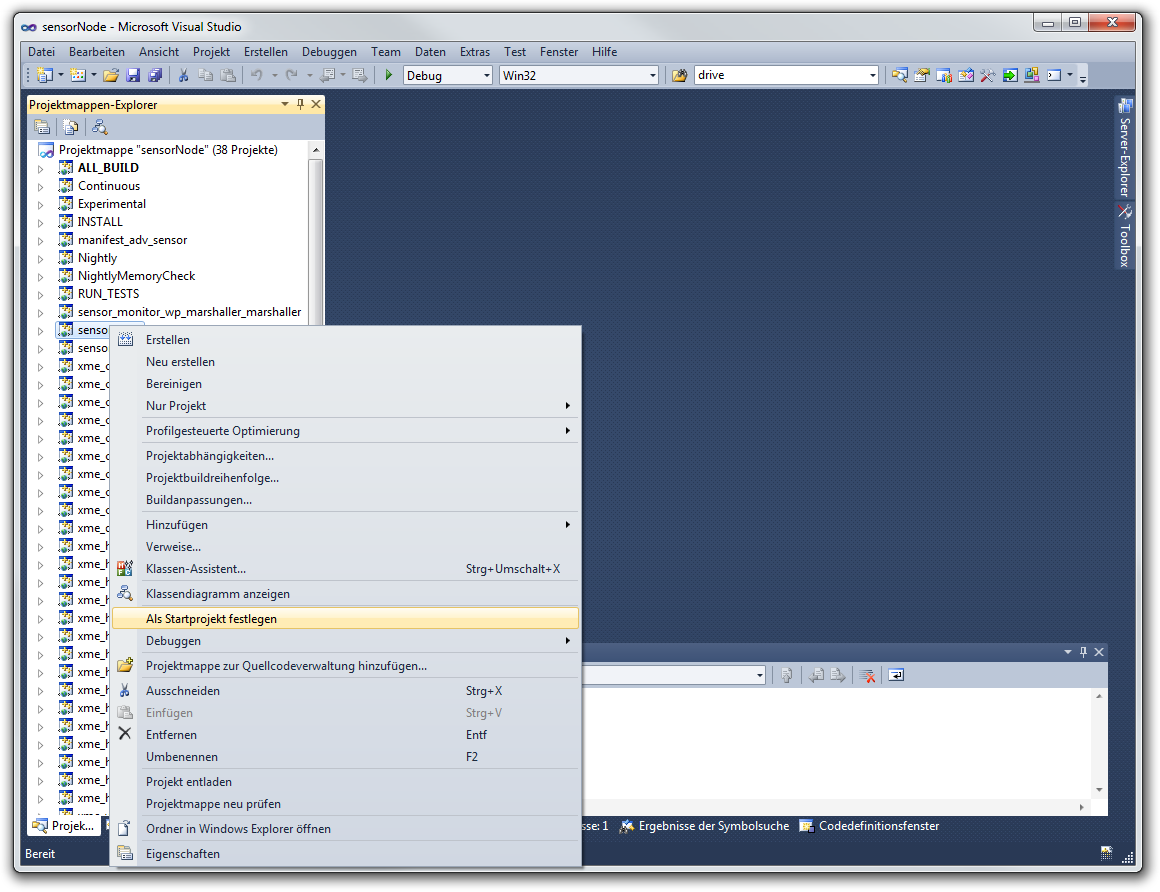
\includegraphics[width=\textwidth]{figures/vs_set_as_startup_project.png}
	\caption{Setting the \texttt{sensorNode} project as \emph{StartUp Project}.}
	\label{fig:vs_set_as_startup_project}
\end{figure}

	\item In the tool bar, select the solution configuration you want to build (usually \texttt{Debug} or \texttt{Release}).
		The \texttt{Debug} build includes debugging information and should be used for development.
		If in doubt, choose \texttt{Debug}.

	\item Hit \emph{F7} to compile the whole solution.

	\item Debug/run the project as usual (e.g., hit \emph{F5} to debug or \emph{Ctrl+F5} to run without debugging).
		If you get prompted whether to rebuild the out-of-date \texttt{ZERO\_CHECK} project (compare Figure~\ref{fig:vs_zero_check}),
		you may select the \emph{Do not show this dialog box again} check box and choose \emph{Yes}.

	\item Continue in Section~\ref{sec:example_sensorMonitor:common}.

\begin{figure}[htpb]
	\centering
	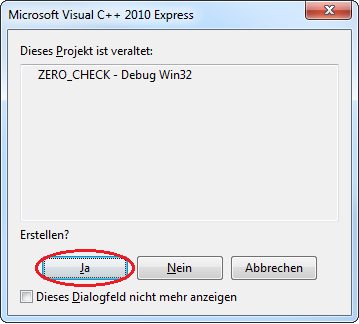
\includegraphics[scale=0.75]{figures/vs_zero_check_edited.png}
	\caption{\texttt{ZERO\_CHECK} project out of date prompt.}
	\label{fig:vs_zero_check}
\end{figure}

\end{enumerate}

\subsection{Notice on Project-global \texttt{CMakeLists.txt} Files}
\label{sec:example_sensorMonitor:projectGlobal}

In \xme, a separate root \texttt{CMakeLists.txt} file is provided for every node.
Thsi is because it could be that each node is to be built for a different target system using a different compiler toolchain.
However, since version 0.8, \xme also support a so-called project-global \texttt{CMakeLists.txt} file per project.
That file is usually located in the root directory of the respective example, say \verb|<XME_ROOT>/examples/sensorMonitor/CMakeLists.txt|.
That file can roughly be undestood as to include all node-specific \texttt{CMakeLists.txt} files.\footnote{%
	With a few exceptions, for example when multiple deployment models exist for a project, see Section~\ref{sec:example_xmt}.%
}
Use the project-global \texttt{CMakeLists.txt} file if all nodes of a project are to be built using the same toolchain for the same target platform.
In this case, it is recommended to name the build directory in the same way as the example itself is named, for example:\\
\verb|<XME_ROOT>/examples/sensorMonitor/build/sensorMonitor|


\subsection{Running the Example Application}
\label{sec:example_sensorMonitor:common}

What you have just compiled is an application that queries simple data from the host it is running on
and makes them accessible to other nodes in the network.
In this case, the collected data is the amount of free space on a certain partition.

When the application starts, you will probably receive a query from the \emph{Windows Firewall}.
\xme is designed to talk to other nodes in the network and hence needs a firewall exception for full functionality.
If you do not want the \xme to talk to other nodes, then simply deny access.\footnote{%
If you want to allow access to the network at a later point in time,
you can change the firewall settings in the \emph{System Control Panel}.}
In this case, communication will be limited to \xme applications on the local computer.
If you want \xme applications to communicate with each other in the local network,
allow access to the \emph{Home or Company Network} as shown in Figure~\ref{fig:firewall_sensorNode}.

\begin{figure}[htpb]
	\centering
	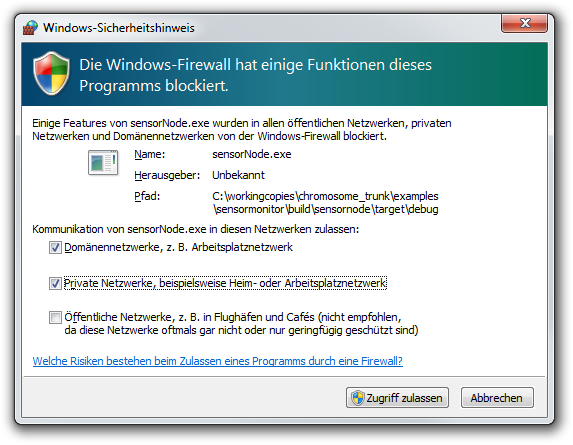
\includegraphics[scale=0.75]{figures/firewall_sensorNode.png}
	\caption{Firewall settings for the \texttt{sensorNode} application.}
	\label{fig:firewall_sensorNode}
\end{figure}

Once the application starts, it presents you with a list of partitions (Linux) or drives (Windows) to choose from.
Select a valid item by entering the respective number.
%
The amount of free space is periodically printed on the console window (compare Figure~\ref{fig:example_sensorNode})
and also transmitted to another \xme node (which is not yet present, see Section~\ref{sec:example_sensorMonitor:monitorNode}).
%
Notice that you can run multiple versions of the sensor node for different partitions/drives on a single host.\footnote{%
	On Windows, when launching the application from within Visual Studio, only one instance can be run at a time.
	In this case, manually navigate to the build directory \texttt{<BUILD\_ROOT>/sensorNode/target} and run the executable from there.
}

The entry point into the executable is in the main source file \verb|<XME_ROOT>/examples/|
\verb|sensorMonitor/src/application/sensorNode/sensorNode.c|,
which also defines the \xme components used in this application.
Notice that this file (and most other files in the example) have been generated from a model.
We will see how this is done in Section~\ref{sec:example_xmt}.
%
%You may now inspect the source code in \verb|sensorNode.c| and the other files related to this example.

\begin{figure}[htpb]
	\centering
	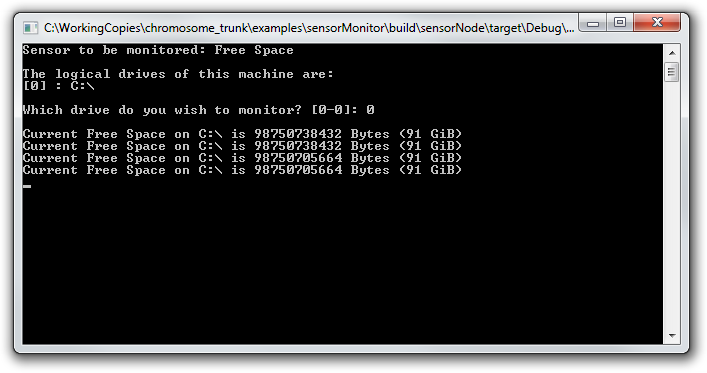
\includegraphics[scale=0.75]{figures/example_sensorNode.png}
	\caption{Sensor node printing free space on drive C: (here on Windows).}
	\label{fig:example_sensorNode}
\end{figure}

\subsection{Compiling and Running the Monitor}
\label{sec:example_sensorMonitor:monitorNode}

Now it's time to compile and run the monitor node that will receive the measurements from the sensor.
Follow the same steps as in Section~\ref{sec:example_sensorMonitor:linux} or Section~\ref{sec:example_sensorMonitor:windows}
(depending on your operating system), but exchange all references to \verb|sensorNode| with \verb|monitorNode|.
On Windows, it is recommended to open a separate Visual Studio instance in order to be able to debug both applications side by side.

When the application starts, you will probably receive another query from the \emph{Windows Firewall}.
Proceed in the same way than for the \verb|sensorNode|.

When launching the \verb|monitorNode| application, you should see the collected data from all sensor nodes on the \emph{current host} being displayed
(compare Figure~\ref{fig:example_monitorNode}).
%
We will shortly come back to remote data transmission in Section~\ref{sec:example_xmt:conclusion}.

\begin{figure}[htpb]
	\centering
	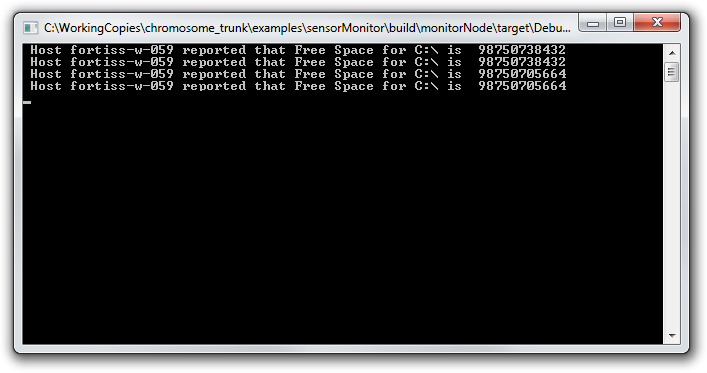
\includegraphics[scale=0.75]{figures/example_monitorNode.png}
	\caption{Monitor node printing free space (here on Windows).}
	\label{fig:example_monitorNode}
\end{figure}

\clearpage
%
% Copyright (c) 2011-2013, fortiss GmbH.
% Licensed under the Apache License, Version 2.0.
% 
% Use, modification and distribution are subject to the terms specified
% in the accompanying license file LICENSE.txt located at the root directory
% of this software distribution. A copy is available at
% http://chromosome.fortiss.org/.
%
% This file is part of CHROMOSOME.
%
% $Id$
%

% =================================================================
\section[Example 2: Code Generation with the Modeling Tool (30 minutes)]{Example 2: Code Generation with the Modeling Tool\\(20 minutes)}
\label{sec:example_xmt}
% =================================================================

Only a fraction of the C code from the last example has actually been written manually.
\xme is released with a model-driven development tool which allows to model an application and subsequently generate code from this model.
The \xme Modeling Tool (XMT) has been implemented in form of an Eclipse\footnote{\url{http://www.eclipse.org/}} plugin.
Refer to appendix~\ref{appx:install_xmt} for a description of how to set up Eclipse and the modeling tool.
From now on we assume that you have successfully installed the tool and have it already running.

The XMT comes with a dedicated perspective, which will open a set of related views and where certain XMT-related commands are activated.
To switch to this perspective go to \textit{Window $\rightarrow$ Perspective $\rightarrow$ Other...} and choose \emph{XMT}.

The sensor/monitor example project from Section~\ref{sec:example_sensorMonitor} was generated from an XMT project.
We will now import the respective example and its models into the Eclipse workspace.
In the menu, choose \textit{File $\rightarrow$ Import...}, open the \emph{General} category and double-click on \emph{Existing Projects into Workspace}.
Make sure \emph{Select root directory} is checked and press the \emph{Browse...} button om the top right.
Select the example directory \verb|<XME_ROOT>/examples/sensorMonitor| and press \emph{OK}.
The project should appear in the list of \emph{projects} and it should be checked (if not, add the check mark).
Make sure that \emph{Copy projects into workspace} is not checked (compare Figure~\ref{fig:xmt_import_sensorMonitor}).
Press \emph{Finish} to import the project, which will show up in the \emph{Project Explorer} pane.

\begin{figure}[htpb]
	\centering
	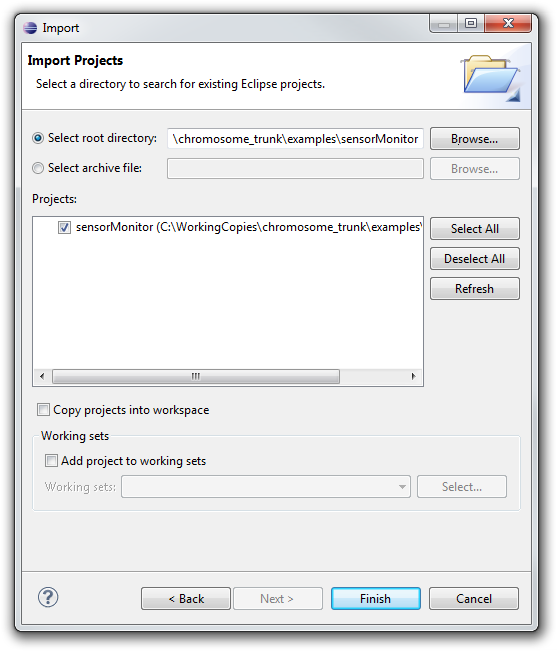
\includegraphics[scale=0.5]{figures/xme_import_sensorMonitor.png}
	\caption{Importing the \emph{sensorMonitor} project into XMT.}
	\label{fig:xmt_import_sensorMonitor}
\end{figure}

\begin{figure}[htpb]
	\centering
	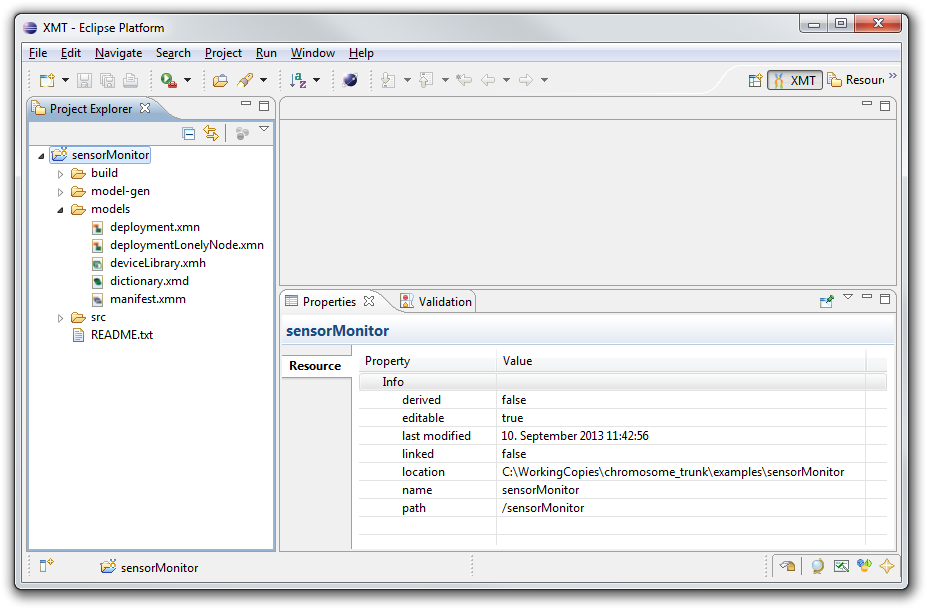
\includegraphics[width=0.9\textwidth]{figures/xmt_project_sensorMonitor.png}
	\caption{XMT perspective of \xme Modeling Tool with imported example project.}
	\label{fig:xmt_project_sensorMonitor}
\end{figure}

You already know the \verb|src/| subdirectory of this example from the previous chapter.
Now we will have a closer look at the \verb|models/| directory, which contains the XMT models that describe this application.
You can see a screenshot of the imported project with expanded models directory in Figure~\ref{fig:xmt_project_sensorMonitor}.
The directory contains five models. 
In the \emph{models} folder we can distinguish four different file extensions:

\begin{itemize}
	\item \emph{xmd} This extension stands for \emph{XMT} topic dictionary, and determines the set of topics and associated attributes to be used for the deployment of components. 
	\item \emph{xmm} This extension stands for \emph{XMT} manifest, and defines components and their interfaces. 
	\item \emph{xmh} This extension stands for \emph{XMT} device types, and is related with hardware-associated properties. 
	\item \emph{xmn} This extension stands for \emph{XMT} deployment model, and defines the mapping of components on devices and the network structure. 
\end{itemize}

In the following subsections we will have a look at these four model types, providing a short description of their purpose and demonstrating how to generate code from them.
As a preparation, we create a backup of the \verb|src/| directory in the project.
Name it something like \verb|src_backup/|. Then delete the original.
We will recreate the content step by step.
Most of the files will be generated completely by the tool.

% ~~~~~~~~~~~~~~~~~~~~~~~~~~~~~~~~~~~~~~~~~~~~~~~~~~~~~~~~~~~~~~~~~~
\subsection{Topic Dictionary}
% ~~~~~~~~~~~~~~~~~~~~~~~~~~~~~~~~~~~~~~~~~~~~~~~~~~~~~~~~~~~~~~~~~~

We begin with the \emph{topic dictionary} model.
A \emph{topic dictionary} is the collection of all topics of an application respectively application domain.
It also holds the \emph{attribute} definitions.
Attributes are attached to topics and specify additional information about the contained data.
%For example the accuracy of a measured value could be defined as an attribute.
%Additionally components can filter for certain attribute values.
%This will be explained in more detail in the chapter about the manifest model.
%\begin{itemize}
% TODO: Move this to manifest, as there are no attribute value definitions in topic dictionaries
%	\item \textbf{Attribute value definition}: The attribute definition explicitly defines pairs of \emph{\textless key, value \textgreater} associated to a topic. 
%        Attribute definitions are associated to publishers in \xme. 
%        Examples of attribute definition could be \emph{data reliability}, \emph{publication rate}, \emph{data measurement unit} or
%        \emph{time to live}. 
%  \item \textbf{Attribute filter}: The attribute filter is associated to subscribers in \xme. A filter defines a set of \emph{\textless key, value, operator\textgreater}
%	      triples, in which the operator is the comparator (\emph{EQUAL, UNEQUAL, GREATER, GREATER\_OR\_EQUAL, SMALLER, SMALLER\_OR\_EQUAL, EXISTS and NOT\_EXISTS})
%				and the value is the value to compare to the attribute definition. 
%\end{itemize}

%Additionally, we can categorize attributes as follows:
% TODO: Mandatory is wrong here, this is called required. Also I do not like this categorization and we might change it in the future...
%
%\begin{itemize}
%	\item \emph{Predefined}: Predefined attributes are specified at design time and associated attribute values do not change during the lifecycle of the application. 
%	\item \emph{Mandatory}: Mandatory attributes define the attributes that should be present in the topic at runtime and they should be provided by the application. 
%	\item \emph{Optional}: Optional attributes are those attributes that can be provided at runtime. These attributes are not mandatory, so they can be provided or not for every topic. 
%\end{itemize}
%
We will check how attributes work in the Plug and Play example (see Section~\ref{sec:example_pnp}). 

\begin{figure}[htpb]
	\centering
	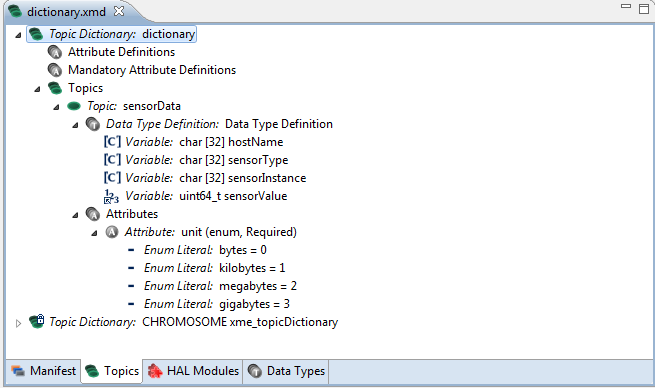
\includegraphics[scale=0.5]{figures/xmt_topicDictionary.png}
	\caption{Topic dictionary model.}
	\label{fig:xmt_topicDictionary.png}
\end{figure}

To open the model, double-click on the file \verb|models/dictionary.xmd| in the project explorer.
An editor window will open that displays the model content in a tree structure~--~see Figure~\ref{fig:xmt_topicDictionary.png}.
Additionally, the \xme \textit{xme\_topicDictionary} shows internal topics used to \xme core components like the \textit{Plug and Play Manager} and \textit{Plug and Play Client}.

You can expand items to see their sub-items.
For example, the item \emph{Topic Dictionary: dictionary} contains an item \emph{Topics} under which you can find the topic definitions.
Remember that a topic defines a type of data that can be sent between components in a \xme network (compare Section~\ref{sec:architecture:glossary}).
Topics can consist of primitive C data types or complex data structures. Additionally, we can define for each topic the set of attributes that apply to that topic. 

A double-click on an item brings the \emph{Properties} view to the foreground.
Here you can see the properties of the selected model item.
Properties may be structured in sub-properties.
When this is he case you can again expand the entry by clicking on the small triangle on the left side.
Figure~\ref{fig:xmt_sub-properties.png} shows an example for the \emph{hostName} variable of the \emph{sensorData} topic.

\begin{figure}[htpb]
	\centering
	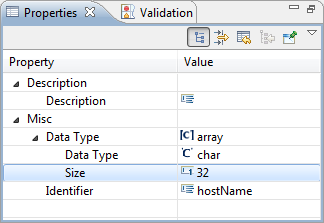
\includegraphics[scale=0.75]{figures/xmt_sub-properties.png}
	\caption{Sub-properties of a data type in the topic dictionary model.}
	\label{fig:xmt_sub-properties.png}
\end{figure}

Now let us have a closer look at the single topic defined in the example, which is called \emph{SensorData}.
In its properties, you can see a description and its name.
You can also see the ID (short for \emph{identifier}) that is used at runtime to identify this topic and its C identifier that will be used in the generated code.\footnote{%
	The identifier is automatically derived from the name of the topic and the name of the dictionary and therefore located in the property category \emph{Read-Only}.
}
Now expand every entry under the topic.
You will see that it has data type definition with several variables.
In the generated code, this will be mapped to a C struct definition.

The SensorData topic also has one attribute called ``\emph{unit}'' which is an enumeration.
It describes the measurement unit of the contained sensor value.
As in our example we measure the free hard disk size,
possible values for this attribute range from \emph{bytes} to \emph{gigabytes}.

\begin{figure}[htpb]
	\begin{minipage}[b]{0.45\linewidth}
		\centering
		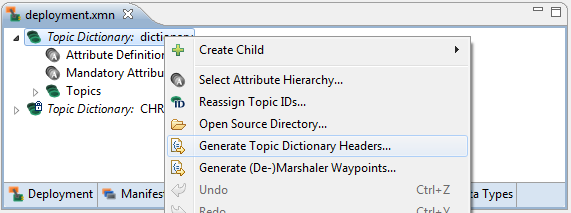
\includegraphics[scale=0.5]{figures/xmt_topicDictionary_gen_headers_a.png}
		\caption{Start topic header generation.}
		\label{fig:xmt_topicDictionary_gen_headers_a}
	\end{minipage}
	\hspace{0.5cm}
	\begin{minipage}[b]{0.45\linewidth}
		\centering
		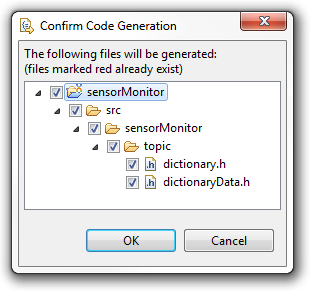
\includegraphics[scale=0.5]{figures/xmt_topicDictionary_gen_headers_b.png}
		\caption{Code generation dialog for topic headers.}
		\label{fig:xmt_topicDictionary_gen_headers_b}
	\end{minipage}
\end{figure}

For a topic dictionary two code generation commands exist.
The first option is to generate the topic headers.
To do this, right-click on the \emph{Topic Dictionary} root element and select \emph{Generate Topic Dictionary Headers...} as shown in Figure~\ref{fig:xmt_topicDictionary_gen_headers_a}.
A dialog will pop up that shows the files that will be generated~--~see Figure~\ref{fig:xmt_topicDictionary_gen_headers_b}.
You can exclude individual files by unchecking them.
Here you can see that this command will generate two files: \texttt{dictionary.h} and \texttt{dictionaryData.h}.
These contain the headers topic identifier and data type definitions that you already know from before.
Select \emph{Overwrite} and press \emph{OK} to generate the files.
After a short moment the Eclipse status line should say \emph{Code generation complete}.
You can navigate to the generated files and have a look at them if you are interested.
If the files are missing in the Eclipse \emph{Project Explorer} pane, try to refresh the \verb|src/| directory
(i.e., right-click and select \emph{Refresh} from the popup menu or select the directory item and press \emph{F5}).

The second generation command \emph{Generate (De-)marshaler waypoints...} creates marshaling and demarshaling functions for the topics of the application.
Different \xme nodes might reside on different target platforms that interpret data differently.
In order to allow these platforms to communicate with each other, the sent data must be converted into a platform independent format.\footnote{%
	For more information, see also \url{http://en.wikipedia.org/wiki/Endianness}.
}
%
The serialization of sent data to this format (i.e., from platform dependent representation to network representation)
is performed by the marshaler; the deserialization respectively by the demarshaler.
The serialization algorithm depends on the sent data~--~and so in our case on the topic definition.
To solve this issue, \xme uses a code generation approach and generates a (de-)marshaler that is specific to a dictionary.
You can start the generation by right-clicking on the \emph{Topic Dictionary} item and select \emph{Generate (De-)Marshaler Waypoints...}.
From the generated files the most interesting ones are the \verb|marshaler.c/h| and \verb|demarshaler.c/h| files, which contain the actual (de-)serialization code.

% ~~~~~~~~~~~~~~~~~~~~~~~~~~~~~~~~~~~~~~~~~~~~~~~~~~~~~~~~~~~~~~~~~~
\subsection{Manifest}
% ~~~~~~~~~~~~~~~~~~~~~~~~~~~~~~~~~~~~~~~~~~~~~~~~~~~~~~~~~~~~~~~~~~

The next model is the so called \emph{manifest}.
A manifest can be considered as a set of component blueprints.
For each component the published and subscribed topics and its functions are defined.
You can create instances of these components later in the \emph{deployment} model.

In order to open the manifest model for the \emph{sensorMonitor} example, double-click on the file \verb|models/manifest.xmm| in the \emph{Project Explorer}.
When you expand the model items, you can see that our manifest contains the several \emph{Sensor} and \emph{Monitor} component types~--~see Figure~\ref{fig:xmt_manifest.png}.
All sensors publish the \emph{sensorData} topic.
The only difference between the different sensor types are their attribute value definitions.
An attribute value definition on a publication sets an attribute of the published topic to a specific value.
This means that all data items produced at runtime will have the corresponding attribute set to the the defined value.
%
\begin{itemize}
	\item The \emph{sensorB} sets the value of attribute \emph{unit} to \emph{bytes}.
	\item The \emph{sensorKB} sets the same attribute to \emph{kilobytes}.
	\item The \emph{sensorMB} sets it to \emph{megabytes}.
\end{itemize}
%
Likewise, monitors subscribe the \emph{sensorData} topic and they differ by their attribute filters.
For example double-click on the filter of \emph{monitorKB}.
In the properties view~~see Figure~\ref{fig:xmt_filterAttributesProperties}~--~you can see the filter specification.
An attribute filter on a subscription specifies that the component is only interested in values where the attribute value satisfies certain criteria (e.g. is equal to a certain value).
%
\begin{itemize}
	\item The \emph{monitorB} component only accepts \emph{sensorData} topic data if the attribute \emph{unit} has its value set to \emph{bytes}.
	\item The \emph{monitorKB} does the same except that the value needs to be \emph{kilobytes}.
	\item The \emph{monitorMB} the same again for \emph{megabytes}.
\end{itemize}
%

\begin{figure}[htpb]
	\centering
	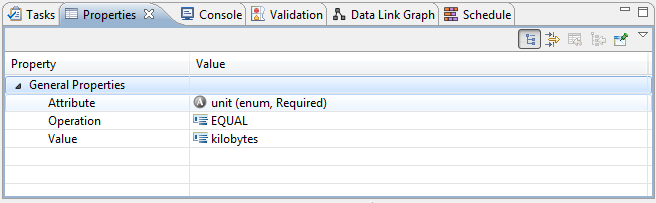
\includegraphics[scale=0.5]{figures/xmt_filterAttributesProperties.png}
	\caption{Attribute filter properties window.}
	\label{fig:xmt_filterAttributesProperties}
\end{figure}

Additionally, there is a manifest called \xme \emph{xme\_manifest} which contains \emph{core} components. 
The code for these components is located in the \verb|<XME_ROOT>/xme/core| directory.
We will not need the core components in this section.

\begin{figure}[htpb]
	\centering
	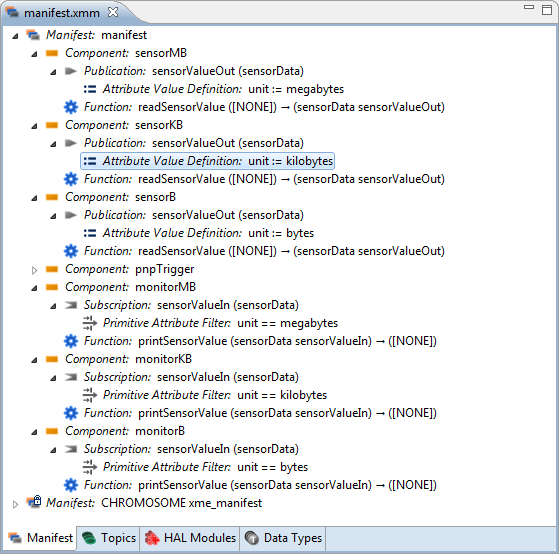
\includegraphics[scale=0.6]{figures/xmt_manifest.png}
	\caption{Manifest model.}
	\label{fig:xmt_manifest.png}
\end{figure}

From the manifest model you can initiate the generation of the so called component and function wrappers and a stub for the function implementation.
Right-click on the \emph{Manifest: sensorMonitor} item and select \emph{Generate Component Wrappers...}.
In the emerging dialog you can see a list of the generated files.

Wrappers constitute the necessary glue code between the function's implementation and the middleware (see also Section~\ref{sec:architecture:glossary}).
These are generated completely from the model and do not need to be adapted.
The files \verb|printSensorValueFunction.c| and \verb|readSensorValueFunction.c| are where the actual functionality of the components are implemented.
Press \emph{OK} to generate all files and open both source files from the \emph{sensorB}.
The generated implementation simply does nothing in its \emph{init()}, \emph{step()} and \emph{fini()} functions.
%
Consider the following excerpt:
%
\begin{lstlisting}[breaklines]
void
sensorMonitor_adv_sensorB_readSensorValueFunction_step
(
	void* param
)
{
    xme_status_t status[1];
    
    sensorMonitor_topic_sensorData_t* portSensorValueOutDataPtr =
        &portSensorValueOutData;
    
    {
        // PROTECTED REGION ID(SENSORMONITOR_ADV_SENSORB_READSENSORVALUEFUNCTION_STEP_C) ENABLED START
\end{lstlisting}
\vspace{-\baselineskip}
\begin{lstlisting}[breaklines, backgroundcolor=\color{yellow}, escapechar=\%]
%%
	// TODO: Auto-generated stub

	XME_UNUSED_PARAMETER(param);
        XME_UNUSED_PARAMETER(status);
%%
\end{lstlisting}
\vspace{-\baselineskip}
\begin{lstlisting}[breaklines]
	// PROTECTED REGION END
    }
	
    status[0] = sensorMonitor_adv_sensorB_sensorBComponentWrapper_writePortSensorValueOut(portSensorValueOutDataPtr);
    
    {
        // PROTECTED REGION ID(SENSORMONITOR_ADV_SENSORB_READSENSORVALUEFUNCTION_STEP_2_C) ENABLED START
\end{lstlisting}
\vspace{-\baselineskip}
\begin{lstlisting}[breaklines, backgroundcolor=\color{yellow}, escapechar=\%]
    
        // TODO: Auto-generated stub
        //       Check return values of writePort calls here
    %%
\end{lstlisting}
\vspace{-\baselineskip}
\begin{lstlisting}[breaklines]
        // PROTECTED REGION END
    }
}
\end{lstlisting}

The \lstinline|// TODO: Auto-generated stub| comments mark where you can add your own implementation of the respective function.
%
In this example, these files are the only thing that you need to manually adjust to recreate the example from the previous chapter.
Just copy these files over from your backup and replace the generated versions.
The code listing above shows the generated \verb|step()| function for the sensor component.

Notice the comments which are marked with \lstinline|// PROTECTED REGION|.
These regions enclose a section of code~--~marked yellow in the code listing~--~that will not be modified by the tool when regenerating the code.
You can verify this by starting the code generation again. Do not modify or remove the protected region comments.
This time before pressing \emph{OK}, have a look at the \emph{Select Merge Strategy} section.
Figure~\ref{fig:xmt_manifest_protected_regions.png} shows the bottom of the code generation dialog with the protected regions strategy highlighted.
This section tells the tool what to do when a generated file already exists.\footnote{%
	Existing files are marked red in the dialog.
}
\begin{enumerate}
	\item The \emph{Compare Editor} option will open a compare editor for every differing file.
		There you can manually select which parts to use from the generated code and which part to keep.

	\item The second option \emph{Protected Regions} will preserve any code in the protected regions.
		Select this option and press \emph{OK}.
	
	\item The third option \emph{Overwrite} will simply overwrite existing files with generated content~--~use with caution.
\end{enumerate}
%
Choose Protected Regions and verify that the content in the protected regions is kept intact.

\begin{figure}[htpb]
	\centering
	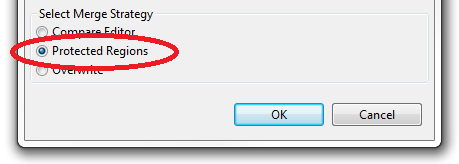
\includegraphics[scale=0.50]{figures/xmt_manifest_protected_regions.png}
	\caption{Code generation dialog with protected region merge strategy selected.}
	\label{fig:xmt_manifest_protected_regions.png}
\end{figure}

% ~~~~~~~~~~~~~~~~~~~~~~~~~~~~~~~~~~~~~~~~~~~~~~~~~~~~~~~~~~~~~~~~~~
\subsection{Device Types}
% ~~~~~~~~~~~~~~~~~~~~~~~~~~~~~~~~~~~~~~~~~~~~~~~~~~~~~~~~~~~~~~~~~~

The \emph{device types} model is a very simple description of hardware devices on which your \xme executables run.
A device type has a \emph{Target Identifier} which specifies the platform (e.g., \emph{posix}, \emph{windows}\footnote{%
	Currently these are the only officially supported platforms.
}).
A device type also has several network interfaces. Currently only \emph{ethernet} is supported.
You will be able to create instances of these devices in the deployment model.

To open the model, double-click on the file \verb|models/deviceTypes.xmn| in the project explorer~--~see Figure~\ref{fig:xmt_deviceTypes.png}.
It contains only a simple device with a single Ethernet interface.
The \emph{target identifier} is deliberately left empty.
In this case, the \xme build system will automatically detect the build environment and assume it to be the execution environment.

\begin{figure}[htpb]
	\centering
	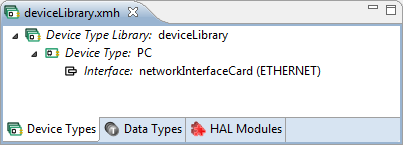
\includegraphics[scale=0.75]{figures/xmt_deviceTypes.png}
	\caption{Device types model.}
	\label{fig:xmt_deviceTypes.png}
\end{figure}

% ~~~~~~~~~~~~~~~~~~~~~~~~~~~~~~~~~~~~~~~~~~~~~~~~~~~~~~~~~~~~~~~~~~
\subsection{Deployment}
% ~~~~~~~~~~~~~~~~~~~~~~~~~~~~~~~~~~~~~~~~~~~~~~~~~~~~~~~~~~~~~~~~~~

The \emph{deployment} model ties everything together.
Here you specify devices and nodes and specify which components are deployed on which node.
In the future you will also be able to specify the network structure here,
which will allow the tool to calculate routes for your network and configure your nodes accordingly.\footnote{%
	Actually you can already define the network structure, but this information is currently not used.
}

To open the model, double-click on the file \verb|models/deployment.xmn| in the project explorer~--~see Figure~\ref{fig:xmt_deployment.png}.
This example contains three nodes.
The \emph{monitorNode} contains the monitor component and the \emph{monitorNode} contains the sensor component.
There are also other components and an additional node that you will get to know in the next chapters.

\begin{figure}[htpb]
	\centering
	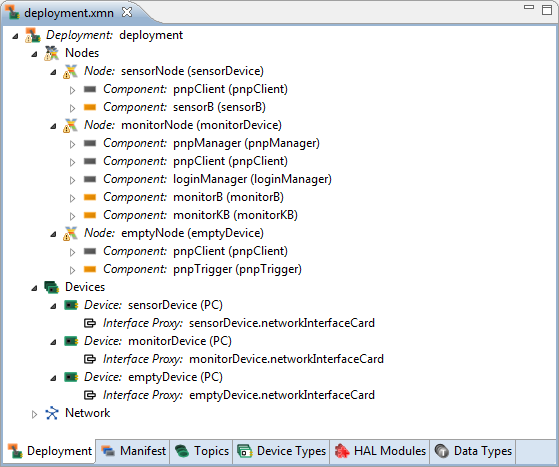
\includegraphics[scale=0.75]{figures/xmt_deployment.png}
	\caption{Fully expanded deployment model.}
	\label{fig:xmt_deployment.png}
\end{figure}

A node here refers to a \xme executable.
Components from the manifests can be instantiated on each node.
You can also instantiate the same component multiple times on the same node (though the example does not include such a case).

A device represents a hardware device on which one or several nodes can be run.
Usually you run only one \xme executable per device, but there might be exceptions.
A device is an instantiation of a type defined in a device types model.
This allows to reuse a device definition.
In addition to the information from the type, you have to specify a network address for each interface.

In the deployment model you can generate the main source file for a node, which will start a \xme instance.
This main source file will also set up the \xme configuration as determined by the tool.
Additionally the CMake scripts are generated that allow you to build your application.
To start the code generation, right-click on the \emph{Deployment: deployment} item and select \emph{Generate Application Code...}
(compare Figure~\ref{fig:xmt_deployment_generate}).
%
\begin{figure}[ht]
	\centering
	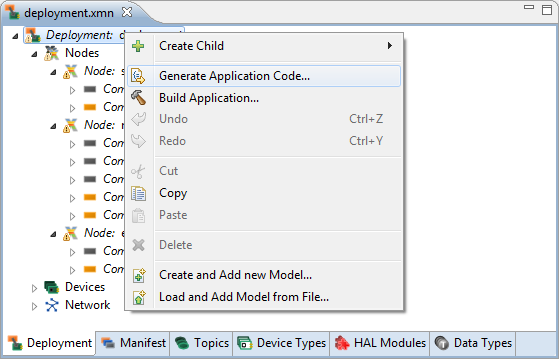
\includegraphics[scale=0.55]{figures/xmt_deployment_generate.png}
	\caption{Generation of application code from a deployment model.}
	\label{fig:xmt_deployment_generate}
\end{figure}
%
There will be three files per node.
The \verb|sensorNode.c| respectively \verb|monitorNode.c| are the aforementioned main source files.
The \verb|CMakeLists.txt| is the main CMake script for the respective node.
The file \verb|CMakeXmeComponents.txt| is included by the main CMake script and contains a definition of all components on that node, so that the build system is aware of them.

When clicking on \emph{Generate Application Code...} you can also see that two new views, called \emph{Data Link Graph} and \emph{Schedule}, pop up.
First let us have a look at the data link graph view.
Screenshot~\ref{fig:xmt_dataLinkGraphView} shows a cutout from this view.
The data link graph is a representation of the resulting data paths in the application.
Beginning from publications and ending at subscriptions it shows the path along which data is sent.
First the XMT searches for matching publications and subscriptions (where the topics are equal and attribute filters match).
For each match a so called logical route is added.
Afterwards these logical routes are refined by adding waypoints.
For example you can have a look at the data path from the publication \verb|sensorB.sensorValueOut| to the subscription \verb|monitorB.sensorValueIn|.
As they lie on different nodes, the data has to be sent across the network.
For this purpose four waypoints have been added, namely: Marshaler, UdpSend, UdpReceive, and Demarshaler.
Data sent from the publication first goes to the Marshaler which serializes the data into a platform independent format.
Next it will be processed by the UdpSend waypoint which sends the data across the network via UDP to the correct receiver(s).
On the receiving node, the UdpReceive waypoint receives the data and passes it to the Demarshaler who deserializes the data again before giving it to the subscription,
where it will be read by the application.

\begin{figure}[ht]
	\centering
	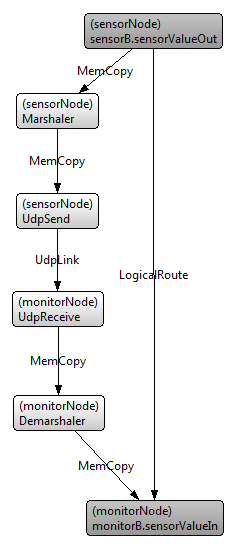
\includegraphics[scale=0.75]{figures/xmt_dataLinkGraphView.png}
	\caption{Cutout from Data Link Graph View.}
	\label{fig:xmt_dataLinkGraphView}
\end{figure}

The other new view is the schedule view.
Here you can see a visualization of the schedule for each node in the deployment model.
For this example it will look like shown in screenshot~\ref{fig:xmt_scheduleView}.
Each node is displayed on a separate line and each line represents one schedule cycle.
Next to the name of a node are colored boxes for each schedule entry.
The purple ones correspond to waypoints, the orange one to functions from components.
The numbers in the boxes are the slot length in milliseconds
and in brackets the number n, where n means that this will be executed only every n-th cycle of the schedule.
The length of a box is proportional to the slot length.
You can hover the mouse cursor over a schedule entry to see a tool tip with more detailed information.

\begin{figure}[ht]
	\centering
	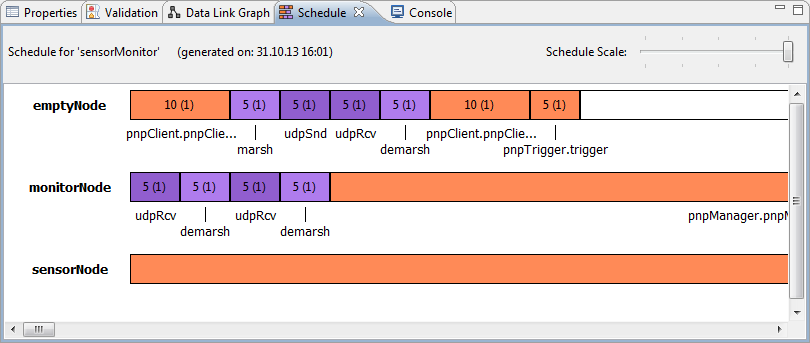
\includegraphics[scale=0.75]{figures/xmt_scheduleView.png}
	\caption{Schedule View.}
	\label{fig:xmt_scheduleView}
\end{figure}

You may now compile the generated code as presented in the previous section or directly use \xmt to build the code as follows:
right-click on the \emph{Deployment: deployment} node in the model
and select \emph{Build Application...}~--~see Figure~\ref{fig:xmt_deployment_generate}.

After clicking on this context menu option, a new window will appear.
This window allows to set up the nodes that are going to be compiled.
The required CMake build system will be automatically created in this case.
%
Note that the nodes that appear in this window are directly related to the deployment model (compare Figure~\ref{fig:xmt_deployment_buildWindow}).
The first option (\emph{Generate Build System}) will generate all the files needed for building the system\footnote{%
	Currently, the build system is associated to a build in Visual Studio.
	In case you want to use a different compiler toolchain, you have to manually adapt the generated \texttt{CMakeLists.txt} file.
}.
The second option is related to with compilation of the generated build.

\begin{figure}[ht]
	\centering
	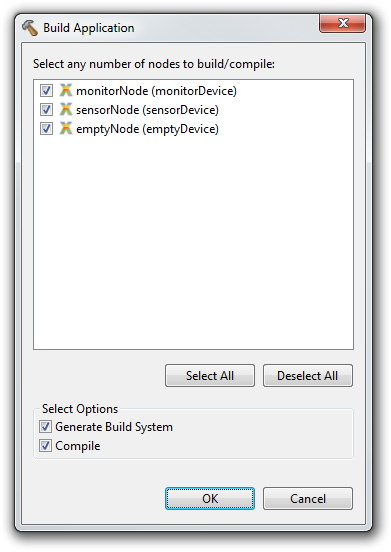
\includegraphics[scale=0.75]{figures/xmt_deployment_buildWindow.png}
	\caption{XMT build options.}
	\label{fig:xmt_deployment_buildWindow}
\end{figure}

% ~~~~~~~~~~~~~~~~~~~~~~~~~~~~~~~~~~~~~~~~~~~~~~~~~~~~~~~~~~~~~~~~~~
\subsection{Conclusion}
\label{sec:example_xmt:conclusion}
% ~~~~~~~~~~~~~~~~~~~~~~~~~~~~~~~~~~~~~~~~~~~~~~~~~~~~~~~~~~~~~~~~~~

If you followed all previous steps, you have generated the complete application and should be able to compile and run it again like described in Section~\ref{sec:example_sensorMonitor}.

Alternatively you can use also trigger compilation from inside the XMT.
For this you first have to enter some CMake related settings.
Go to \textit{Window $\rightarrow$ Preferences}.
In the preferences dialog expand the \textit{XMT} item and click on the sub-item \textit{CMake}.
Set the path to the CMake executable by pressing \emph{Browse...} and navigating to the respective file.
Then choose the correct generator from the drop-down list.
You only have to do these steps once.
Now you can trigger build system generation and compilation.
Go to the deployment model and right-click on the deployment item.
Choose \emph{Build Application...}.
Select the nodes that you want to build and check if you want to generate the build system or compile the selected nodes (or both).
When pressing \emph{OK} the tool will start CMake and print its output to the Console view.

You are now free to modify the models, re-generate the source code and change the behavior of the components.
One interesting example is to change the IP addresses of the nodes and deploy them on different machines in a local-area network.
Notice however that you might need to add respective exceptions in your firewall.
The default ports being used in this example are 33221 for \textit{monitor} node, 33222 for \textit{sensor} node and 33223 for \textit{empty} node.
More on the topic of distributed applications will come in the next release of \xme (see our roadmap in Appendix~\ref{appx:roadmap}).

\clearpage
%
% Copyright (c) 2011-2013, fortiss GmbH.
% Licensed under the Apache License, Version 2.0.
% 
% Use, modification and distribution are subject to the terms specified
% in the accompanying license file LICENSE.txt located at the root directory
% of this software distribution. A copy is available at
% http://chromosome.fortiss.org/.
%
% This file is part of CHROMOSOME.
%
% $Id$
%

% =================================================================
\section{Example 3: Plug~\&~Play Showcase (30 minutes)}
\label{sec:example_pnp}
% =================================================================

In Section~\ref{sec:architecture}, we shortly explained the planned plug~\&~play features of \xme.
The current version implements both plug~\&~play and login features.
The following showcase illustrates the current state of plug~\&~play implementation.

This example is again based on the previous sensor/monitor example and extends it.
The goal is to activate a new sensor component on a third node called ''\emph{emptyNode}'' and a new monitor on a fourth node called ''\emph{monitorKB}''.
The \emph{emptyNode} is targeted to demonstrate the plug~\&~play and login capabilities in \xme, while \emph{monitorKB} is targeted to demonstrate 
the attribute support during plug~\&~play phase. 

In this case, we will use attributes to demonstrate data filtering during plug~\&~play phase of \xme. For this purpose, we differentiate
between the \emph{monitorNode}, containing one \emph{monitorB} component that filters sensing data received with the measurement unit
established to \emph{bytes}, and one \emph{monitorKB} component that filtering data measured in \emph{kilobytes}.

Hence, after the plug~\&~play phase is finished, the \emph{monitorB} component on \emph{monitorNode} will receive values from the \emph{sensorB} component placed on
\emph{sensorNode}, and the \emph{monitorKB} component on \emph{monitorNode} is going to receive sensing data from \emph{sensorKB} component located on \emph{emptyNode}.
The first sensing data is measured in \emph{bytes}, while the latter is measured in \emph{kilobytes}.

Additionally, in order to demonstrate logout capabilities, it is explained how the system reacts to a node logout received from ''\emph{emptyNode}''. 


\subsection{Adding the emptyNode}

The \emph{emptyNode} is already defined in the deployment model.
Open the model with the \emph{XMT} tool to have a look at it\footnote{See previous example how to do this.}~--~compare Figure~\ref{fig:pnp_deployment}.
The assignment of nodes to components is as follows:
\begin{itemize}
	\item[] \textbf{monitorNode:} \emph{loginManager}, \emph{pnpManager}, \emph{pnpClient}, \emph{monitorB} (displays bytes) and \emph{monitorKB} (displays kilobytes).
	\item[] \textbf{sensorNode:} \emph{pnpClient} and \emph{sensorB}.
	\item[] \textbf{emptyNode:} \emph{pnpClient} and \emph{pnpTrigger}.
\end{itemize}

\begin{figure}[htpb]
	\centering
	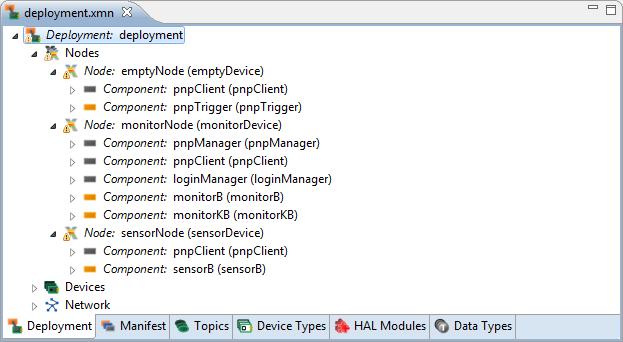
\includegraphics[width=0.9\textwidth]{figures/pnp_deployment.png}
	\caption{Deployment model highlighting the emptyNode.}
	\label{fig:pnp_deployment}
\end{figure}

The \emph{pnpTrigger} on \emph{emptyNode} is an example of a tutorial-specific component performing the following actions:
\begin{itemize}
	\item[] Requests the automatic instantiation of a \emph{sensorKB} component after the \emph{emptyNode} is logged-in.
	\item[] Request the logout of the \emph{emptyNode} after having demonstrated the other features. 
\end{itemize}

In this subsection, the objective is to demonstrate dynamic plug-in of the \emph{sensorKB} component. 
The latter will be demonstrated in the following subsection. 

%A \emph{Plug~\&~Play Client} component listens for commands to install and run new components on their node.\footnote{Currently this is only possible for the sensor and monitor components.}
%TODO: Remove from here and place it in the corresponding section (e.g. Architectures). 
%In future versions of \xme, the client will also be able to uninstall and transfer components from one node to another.

%The component which issues these commands is the \emph{Plug~\&~Play Manager}.

The \emph{Plug~\&~Play Manager} component exists at most once in a \xme network.
This component communicate with \emph{Login Manager} to provide authorization to establish connection between nodes that are already logged in.

%TODO: DISABLED FOR 0.6 REL, BECAUSE THE SCENARIO HAS CHANGED!
%The first step is sending a broadcast \emph{login request} message from the \emph{emptyNode}. The node owning the \emph{Login Manager}
%(currently \emph{monitorNode}) receives the request and process this request\footnote{In the future this will include credential, handshake or other
%security mechanisms to ensure that the requesting node can join to the network.}. 
%After checking credentials\footnote{Credential checking needs the modification of corresponding topic, and the existence of a credential checked in the system. This will be implemented in the future.}, 
%the \emph{Login Manager} communicates with the \emph{Plug~\&~Play Manager} to grant the access to the \emph{emptyNode}
%to create new components instances and the corresponding data links. 
%Finally, the \emph{Login Manager} sends a \emph{login response} to the \emph{emptyNode}. After receiving this login confirmation, 
%the \emph{emptyNode} will be able to publish its \emph{component instance manifest} with all components that it wants to deploy at runtime. 
%
%The \emph{Component Instance Manifest} is the topic exchanged between \emph{Plug \& Play Client} and \emph{Plug \& Play Manager}
%with the components already running on \emph{emptyNode} and the components that want to be deployed dinamically by the \emph{emptyNode}.
%In our case, we want to deploy dinamically one single components: a \emph{sensorKB} component. 
%Therefore this \emph{Component Instance Manifest} is sent from the \emph{Plug \& Play Client} running in the \emph{emptyNode} to
%the \emph{Plug \& Play Manager} running in the \emph{monitorNode}.
%
%When the \emph{Plug \& Play Manager} receives this \emph{Component Instance Manifest}, the Plug~\&~Play Manager checks this manifest and triggers the following components:
%\begin{itemize}
	%\item The \emph{Logical Route Manager} is asked for logically feasible routes between existing and new components.
	%\item The \emph{Network Configuration Calculator} is triggered for the logically feasible routes
		%in order to calculate transport mechanisms (\emph{waypoints}) for the logical routes (for example using UDP communication).
%\end{itemize}
%
%The respective outcome is then forwarded to the individual \emph{Plug~\&~Play Client} components in the affected nodes
%in order to implement the required changes.

%In this (preliminary) example, the command to activate the new sensor component is sent in the \texttt{\_step()} function of the Plug~\&~Play Manager.
%This code is already present, but has been commented out.
%We will reactivate it as follows:
%Open the following file:
%
%\begin{itemize}
%	\item[] \texttt{<XME\_ROOT>/examples/sensorMonitor/src/sensorMonitor/adv/pnpManager/src/}\\
%\texttt{pnpManagerFunction.c}.
%\end{itemize}
%At the top of the file, you will find the following code snippet:
%
%\begin{lstlisting}[breaklines]
%// PROTECTED REGION ID(SENSORMONITOR_ADV_PNPMANAGER_PNPMANAGERFUNCTION_C_INCLUDES) ENABLED START
%#include "xme/core/manifestRepository/include/manifestRepository.h"
%#include "xme/core/directory/include/plugAndPlayManager.h"
%\end{lstlisting}
%\vspace{-\baselineskip}
%\begin{lstlisting}[breaklines, backgroundcolor=\color{yellow}, escapechar=\%]
%//#define ENABLEPNP
%\end{lstlisting}
%\vspace{-\baselineskip}
%\begin{lstlisting}[breaklines]
%// PROTECTED REGION END
%\end{lstlisting}
%
%\noindent Change the line highlighted in yellow to (i.e., remove the slashes at the beginning of the line):

%\begin{lstlisting}[breaklines, backgroundcolor=\color{yellow}, escapechar=\%]
%#define ENABLEPNP
%\end{lstlisting}

%This is all you need to do to enable the plug~\&~play showcase.
%Now follow these steps to run it:
Refer to Section~\ref{sec:example_sensorMonitor} for instructions on how to set up the build environment and build the code.
To run this example, follow these steps:

\begin{enumerate}
	\item First start the \emph{monitorNode}. This node contains four key components relevant to plug~\&~play and login process:
		\begin{itemize}
			\item A \emph{monitorB} component, subscribed to any \emph{sensorData} topic sensing data measured in \emph{bytes}.
			\item A \emph{monitorKB} component, subscribed to any \emph{sensorData} topic sensing data measured in \emph{kilobytes}.
			\item A \emph{pnpClient} component, listening to requests from \emph{pnpManager} component.
			\item A \emph{pnpManager} component, which orchestrates the plugin process of additional components to the network, and communication with the \emph{loginManager}
			  to grant access to already logged in nodes.
			\item A \emph{loginManager} component, which receives requests broadcasted by \emph{Login Client} component and delivers login responses to nodes which requested to login.
		\end{itemize}
	\item Start the \emph{sensorNode}. The \emph{sensorNode} contains two components at startup:
		\begin{itemize}
			\item A \emph{pnpClient} component, listening to requests from \emph{pnpManager} in the network.
			\item A \emph{sensorB} component, emitting sensor data in \emph{bytes}.
		\end{itemize}
		Like in the previous examples, the \emph{sensorB} component will ask you which partition to monitor
		(compare Figure~\ref{fig:example_pnp_sensorNode}).
		Choose any partition that you want. This will initiate the data production on the sensor side.
		As we do not have yet any subscriber for the data, the data is not received by any other component.
	\item Finally, start the \emph{emptyNode}. This \emph{emptyNode} contains two components:
		\begin{itemize}
			\item A \emph{pnpClient} component, in charge of sending \emph{component instance manifests} and listening to requests from \emph{pnpManager}.
			\item A \emph{pnpTrigger} component, a tutorial-specific component to demonstrate over the time the plug-in of one sensor component and the logout of the \emph{sensorNode}.
		\end{itemize}
		%The \emph{emptyNode} is started with the \emph{pnpTrigger} that sends a plug~\&~play request after 5 execution cycles and 
		%a \emph{pnpClient} to send component instance manifests to and to listening to requests from \emph{pnpManager}.
		%Notice that nothing is happening yet (the console window stays blank), because there exists no \emph{pnpManager} component sending requests to this node.
\end{enumerate}	
		
The logical steps when \emph{emptyNode} is running are as follows:
\begin{enumerate}
	\item After five execution cycles, the \emph{pnpTrigger} calls a function in the \emph{pnpClient} to trigger the initiate the plug-in process for a \emph{sensorKB} component in the \emph{emptyNode}.
	\item The \emph{pnpClient} on \emph{emptyNode} sends a \emph{Component Instance Manifest} topic message to the \emph{pnpManager} on \emph{monitorNode}
		to request that the \emph{sensorKB} component should be added.
	\item The \emph{pnpManager} receives the \emph{Component Instance Manifest} and process its content.
	\item The \emph{pnpManager} component calculates internally matches between subscriptions and publications with the
		current registered nodes and components (compare Figure~\ref{fig:example_pnp_monitorNode}). Additionally, for every matching topic,
		the attribute filter in subscription should match with attribute definitions associated to that topic in publications.
	\item A logical and physical route is calculated by the \emph{pnpManager} component, and the result is sent to the corresponding nodes.
	  In our case, the logical route for the \emph{sensorData} topic between the \emph{sensorKB} component specification on \emph{emptyNode}
		and the \emph{monitorKB} running component on \emph{monitorNode} is returned back as the result of plug~\&~play process.
	\item After receiving the \emph{runtime graph} topic on \emph{emptyNode}, the \emph{sensorKB} component is scheduled and starts running and ask you which partition to observe.
		Choose any partition~--~preferably other different partition than the other selected on \emph{sensorNode}.
		After this, the data production for \emph{sensorData} topic is delivered.
	\item After receiving the \emph{runtime graph} topic on \emph{monitorNode}, the \emph{monitorKB} component is scheduled and starts running receiving \emph{sensorData} expressed in \emph{kilobytes}.
	\item After this, both sensors (i.e., \emph{sensor ~--~in bytes~--~ on \emph{SensorNode}} and the newly created \emph{sensor} ~--~in kilobytes~--~ on the (formerly) \emph{emptyNode})
		send their measurements to the \emph{monitorB} and \emph{monitorKB} components located on \emph{MonitorNode}.
		Check the \emph{monitorNode} console window.
\end{enumerate}

\begin{figure}[htpb]
	\centering
	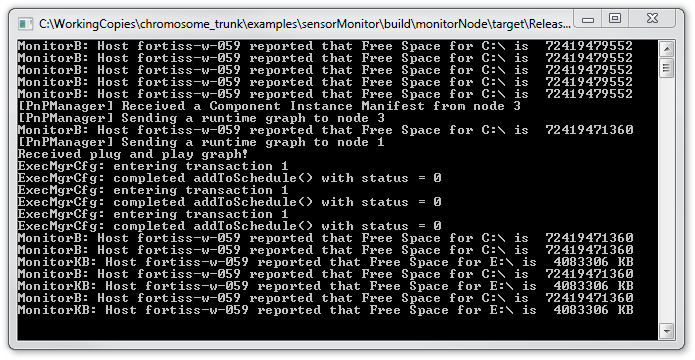
\includegraphics[scale=0.7]{figures/example_pnp_monitorNode.png}
	\caption{Console window of \emph{monitorNode} during plug~\&~play.}
	\label{fig:example_pnp_monitorNode}
\end{figure}

\begin{figure}[htpb]
	\centering
	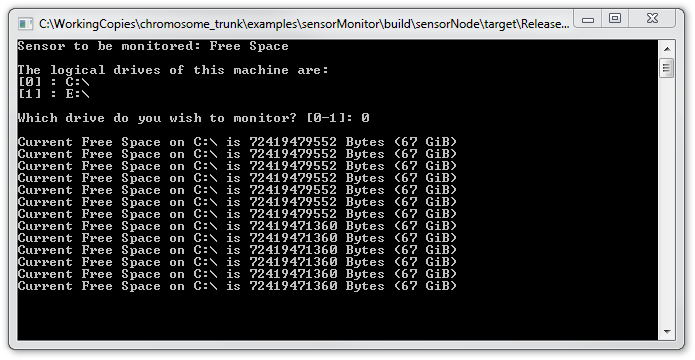
\includegraphics[scale=0.7]{figures/example_pnp_sensorNode.png}
	\caption{Console window of \emph{sensorNode}.}
	\label{fig:example_pnp_sensorNode}
\end{figure}

\begin{figure}[htpb]
	\centering
	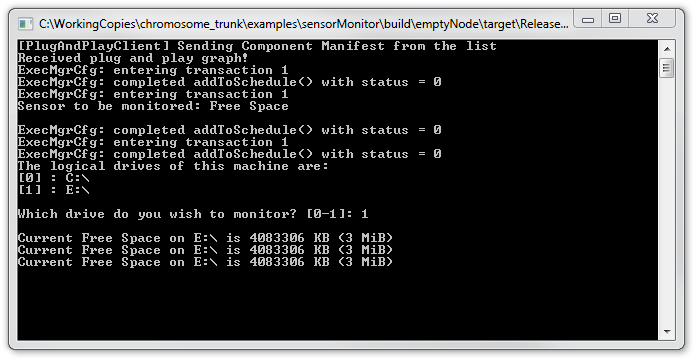
\includegraphics[scale=0.7]{figures/example_pnp_emptyNode.png}
	\caption{Console window of \emph{emptyNode} during plug~\&~play.}
	\label{fig:example_pnp_emptyNode}
\end{figure}

There is still one more node that can be added at runtime to the system, the \emph{lonelyNode}. 
We will explore how to integrate external nodes developed outside the common shared deployment model on \emph{XMT}.

\subsection{Self-initiated logout process for emptyNode}

In this subsection, it is explained the logout process for a given node, and how to communicate the logout of this node to other running nodes. 

This logout process for \emph{emptyNode} is a continuation of the execution of the plug-in example of the previous section. 
The responsible component for initiating the logout process is \emph{pnpTrigger}. The logout process will start after fifty execution cycles. 

For the execution of this example, it is expected that the user have already started the \emph{monitorNode}, the \emph{sensorNode} and the \emph{emptyNode}, as described in the previous section. 

The logout process for \emph{emptyNode} is executed as follows:
\begin{enumerate}
  % Step 0
	\item The \emph{pnpTrigger} requests to \emph{pnpClient} to trigger the logout process for the current node (in this case, the \emph{emptyNode}).
	% Step 1
	\item The \emph{pnpClient} generates a logout topic message. This logout topic message is delivered through the network to the \emph{pnpManager} on the \emph{monitorNode}.
	\item The \emph{pnpManager} receives the logout message with the node identifier. This will unannounce the node-associated componnent from \emph{pnpManager} (and thus, component ports from \emph{Logical Route Manager}, and calculates the logical routes to be removed. 
	\item At this point, there are two different set of logical routes:
	\begin{itemize}
		% Step 3.a
		\item The routes of subscribers obtaining data from the node to disconnect from \xme (\emph{emptyNode}). These nodes will receive a \emph{runtime graph} with the directive of removing all physical routes connected to the \emph{emptyNode}.
		% Step 3.b
	  \item The \emph{emptyNode} will receive all the connected physical routes (subscribers and publishers) to other nodes. 
	\end{itemize}
	\item The \emph{pnpClient} components in another nodes than \emph{emptyNode}, will reconfigure the scheduling to eliminate the subscription listening coming from \emph{emptyNode} and the publication of messages targeted to \emph{emptyNode}.
	\item The \emph{pnpClient} component in \emph{emptyNode}, will receive the confirmation that it can be disconnected safely from \xme. Before this complete disconnection, removes all schedules associated to publications and subscriptions, and sends an acknowledgement signal back to \emph{pnpManager}.
\end{enumerate}
		
\subsection{Third-party initiated logout process for sensorNode}

The logout process for \emph{sensorNode} is executed in the same was as the logout process in \emph{emptyNode}, with the difference which the process is directly triggered from \emph{pnpTrigger} component in \emph{monitorNode}. The logout process from \emph{pnpTrigger} will start after the seventieth execution cycle. This \emph{pnpTrigger} on \emph{monitorNode} calls directly the logout function in the \emph{pnpManager} to initiate the logout for node \emph{sensorNode}. The following steps are equal to the previous logout process. 

In this section, it was demonstrated how to connect and execute non-previously defined components in \xme (plug~\&~play), and how to disconnect nodes from the infrastructure at runtime (node logout). 
\clearpage
%
% Copyright (c) 2011-2013, fortiss GmbH.
% Licensed under the Apache License, Version 2.0.
% 
% Use, modification and distribution are subject to the terms specified
% in the accompanying license file LICENSE.txt located at the root directory
% of this software distribution. A copy is available at
% http://chromosome.fortiss.org/.
%
% This file is part of CHROMOSOME.
%
% $Id$
%

% =================================================================
\section{Example 4: Integrating External Nodes (20 minutes)}
\label{sec:example_lonelyNode}
% =================================================================

In previous examples, we have generated the code for nodes that have been modeled within the same deployment model in \xmt.
These nodes were hence known a priori and the generated code is based on this knowledge.
This allows to establish all connections from the start.

However, this scenario does not always apply.
In case we want to add a new node to an already existing ecosystem of nodes,
the new node needs to be developed independently from current established nodes.
%
In this example, we will generate a new deployment model without having information about nodes that are already running in \xme.

For modeling the firmware of the new node called \emph{Lonely Node}, we again use \xmt.
For this purpose, we will start again the Eclipse workspace and import the deployment model
\emph{deploymentLonelyNode.xmn} located at \verb|<XME_ROOT>/examples/sensorMonitor| (compare Figure~\ref{fig:xmt_deploymentLonely}).
%
You should note that if you have already imported all models in previous example,
the \emph{lonely node} will be already imported in your workspace.

\begin{figure}[htpb]
	\centering
	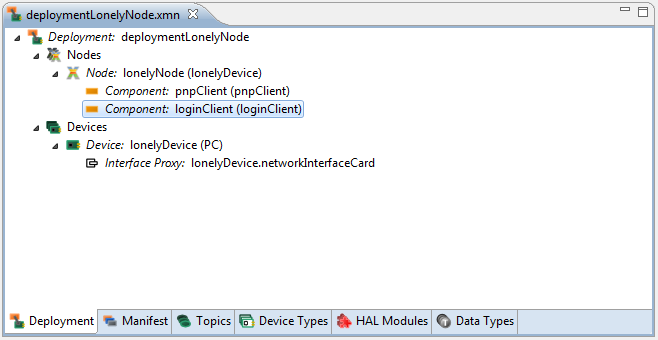
\includegraphics[scale=0.5]{figures/xmt_deploymentLonely.png}
	\caption{Lonely Node deployment model.}
	\label{fig:xmt_deploymentLonely}
\end{figure}

We assume here that the code for running the \emph{monitorNode}, \emph{sensorNode} and \emph{emptyNode} is already generated and compiled.
In case that this is not yet the case, please follow the steps explained in the example in Section~\ref{sec:example_xmt} before continuing.

% ~~~~~~~~~~~~~~~~~~~~~~~~~~~~~~~~~~~~~~~~~~~~~~~~~~~~~~~~~~~~~~~~~~
\subsection{Overview of lonelyNode}
% ~~~~~~~~~~~~~~~~~~~~~~~~~~~~~~~~~~~~~~~~~~~~~~~~~~~~~~~~~~~~~~~~~~

For the deployment model of \emph{lonely node}, we already use generated components which are part of \xmt, such as \emph{loginClient} and \emph{pnpClient}.
These two components play the following roles in this scenario:

\begin{itemize}
	\item The \emph{loginClient} component establishes a connection with the \emph{Login Manager}
		(here running on the \emph{monitorNode}) in order to register the \emph{lonelyNode}.
	
	\item After login is completed, the \emph{pnpClient} component announces the application components
		running on the \emph{lonelyNode} to the \emph{Plug and Play Manager} (also running on the \emph{monitorNode}).
		\emph{Plug and Play Manager} will then establish the required communication routes.
\end{itemize}
%
For more information about how the login and plug~\&~play infrastructure works, please refer to Section~\ref{sec:example_pnp}.

As it is generated from \xmt, the lonely node contains the code for starting an \xme instance of this node.
However, as the lonely node does not contain any information about configurations of already running nodes --
for example it does not know where the \emph{Login Manager} is located --
it needs to discover the network configuration for using the login and plug~\&~play services.

The login operation is performed using broadcasting of a login request and the plug~\&~play operation is completed using the configuration
received from the login response, which contains the interface address where the \emph{Plug and Play Manager} is listening to \emph{component instance manifests}.

Now let's generate the code for \emph{lonelyNode}:
just like in the previous example, right-click on the \emph{Deployment: deploymentLonelyNode} in the deployment model
and click on \emph{Generate Application Code...}~--~see Figure~\ref{fig:xmt_deploymentLonely_generate}.
Confirm the code generation dialog accordingly.

\begin{figure}[ht]
	\centering
	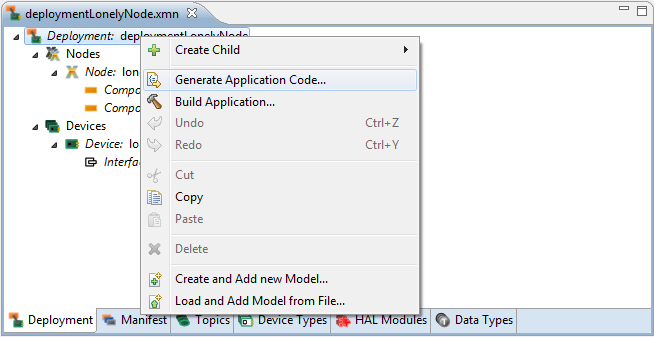
\includegraphics[scale=0.5]{figures/xmt_deploymentLonely_generate.png}
	\caption{Generation of application code for \emph{lonelyNode}.}
	\label{fig:xmt_deploymentLonely_generate}
\end{figure}

In order to compile the generated code, right-click on the \emph{Deployment: deploymentLonelyNode}
and select \emph{Build Application...}~--~see Figure~\ref{fig:xmt_deploymentLonely_build}.

\begin{figure}[ht]
	\centering
	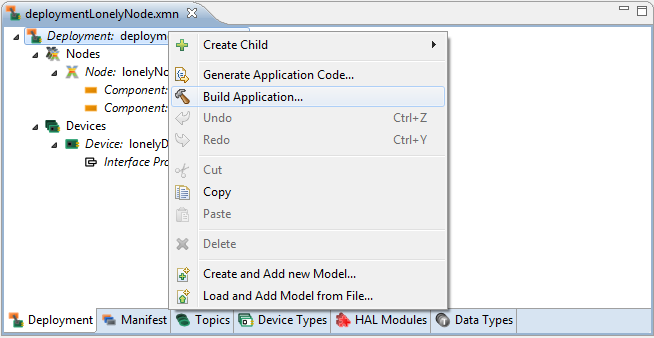
\includegraphics[scale=0.5]{figures/xmt_deploymentLonely_build.png}
	\caption{Build of application code for \emph{lonelynode}.}
	\label{fig:xmt_deploymentLonely_build}
\end{figure}

In the build window, select \emph{lonelyNode} and check \emph{Generate Build System} and \emph{Compile}
as shown on Figure~\ref{fig:xmt_deploymentLonely_buildWindow}.
Then click \emph{OK}.

\begin{figure}[ht]
	\centering
	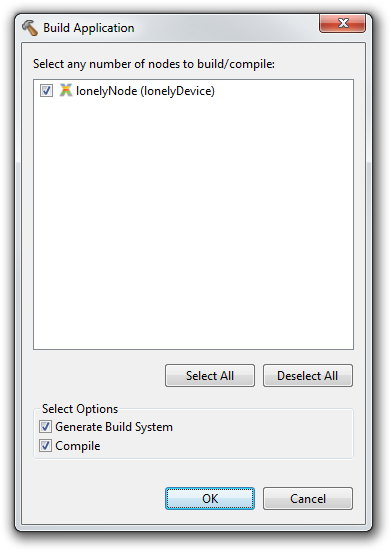
\includegraphics[scale=0.75]{figures/xmt_deploymentLonely_buildWindow.png}
	\caption{XMT build options for lonely node.}
	\label{fig:xmt_deploymentLonely_buildWindow}
\end{figure}

The output of the build is created in the \verb|build/lonelyNode| folder inside the \emph{sensorMonitor} project in the workspace.

% ~~~~~~~~~~~~~~~~~~~~~~~~~~~~~~~~~~~~~~~~~~~~~~~~~~~~~~~~~~~~~~~~~~
\subsection{Running the lonelyNode}
% ~~~~~~~~~~~~~~~~~~~~~~~~~~~~~~~~~~~~~~~~~~~~~~~~~~~~~~~~~~~~~~~~~~

After compilation is finished, the \emph{lonelyNode} is ready to run.
Before of running the executable, make sure that at least the node containing \emph{Login Manager} and the \emph{Plug~\&~Play Manager} is currently running.
If you followed the instructions in this tutorial, that node is the \emph{monitorNode}.

\emph{lonelyNode} includes in the manifests for deploying one \emph{sensorB} component.\footnote{%
	The pnpClient will announce any component type listed in the \emph{pluggable components} attribute of its node. For lonely node this list only contains a \emph{sensorB}.
}
To run the lonely node, just double-click on Eclipse workspace file \verb|/build/lonelyNode/target/Debug/|
\verb|lonelyNode.exe|.
%
As soon as the node is started, it should emit login requests that are handled by the \emph{Login Manager}.
After a couple of seconds, login should be complete and the component manifest exchanged.
Then, \emph{Plug and Play Manager} should update the communication routes such that
the \emph{sensorB} on \emph{lonelyNode} sends its data to the \emph{monitorB} on \emph{monitorNode}
(compare Figure~\ref{fig:example_lonelyNode}).
%

%In the case we are running all four nodes (\emph{monitorNode}, \emph{sensorNode}, \emph{emptyNode} and \emph{lonelyNode}),
%the \emph{lonelyNode} will publish sensor data to \emph{monitorNode} and in \emph{emptyNode}, and will subscribe to sensing data published by \emph{sensorNode} and \emph{emptyNode}.
%Additionally, the \emph{monitor} in \emph{lonelyNode} will receive publications produced by \emph{sensor} on \emph{lonelyNode}.

\begin{figure}[htpb]
	\centering
	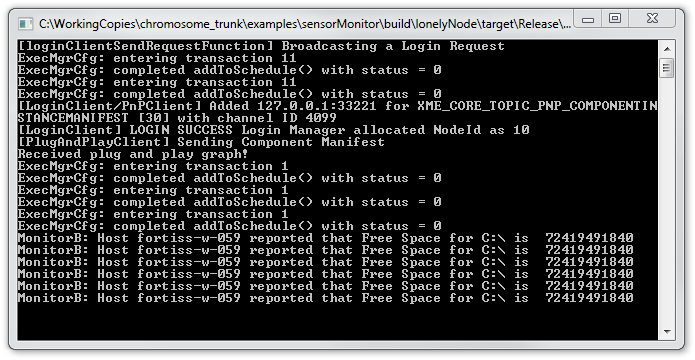
\includegraphics[scale=0.7]{figures/example_lonelyNode.png}
	\caption{Console window of \emph{lonelyNode} during login and plug~\&~play.}
	\label{fig:example_lonelyNode}
\end{figure}

% ~~~~~~~~~~~~~~~~~~~~~~~~~~~~~~~~~~~~~~~~~~~~~~~~~~~~~~~~~~~~~~~~~~
\subsection{Conclusion}
\label{sec:example_lonelyNode:conclusion}
% ~~~~~~~~~~~~~~~~~~~~~~~~~~~~~~~~~~~~~~~~~~~~~~~~~~~~~~~~~~~~~~~~~~

In this example, we have generated code for a new node which is developed completely independent from from the other nodes in the network.
The only shared specification between the nodes is the topic dictionary, which defines the structure of the data being exchanged.
%
The newly node, named \emph{lonelyNode}, completes its registration in \emph{Login Manager} component
located at \emph{monitorNode} (or any other node containing the \emph{Login Manager}),
exports its \emph{component instance manifest} to the \emph{Plug and Play Manager},
and -- in this case -- starts the components \emph{sensor} and \emph{monitor} after successful login.
%
In this example, you learned how to develop a new component from scratch, without any connection to an existing infrastructure of \xme.

\clearpage
%
% Copyright (c) 2011-2013, fortiss GmbH.
% Licensed under the Apache License, Version 2.0.
% 
% Use, modification and distribution are subject to the terms specified
% in the accompanying license file LICENSE.txt located at the root directory
% of this software distribution. A copy is available at
% http://chromosome.fortiss.org/.
%
% This file is part of CHROMOSOME.
%
% $Id: example_helloworld.tex 5238 2013-09-30 15:44:39Z ruiz $
%

\section{Example 5: Calculator Server (15 minutes)}
\label{sec:example_calculator}

The next example demonstrates the use of an alternative communication pattern provided by \xme,
the so-called request/response (or RR) style of communication.
In contrast to publish/subscribe, which has basically a fire \& forget semantics,
RR works more like client/server:
components can send \emph{requests} that can be processed by one or more \emph{request handlers}.
On success, the request handler sends a \emph{response} back to the component that issued the request.

For this purpose, two topics are required: a request topic and a response topic.
A data packet of type request is sent from the client to the server ``on demand''
and contains all information necessary for the server to process the request.
Subsequently, the server shall reply with a data packet of type response, which contains the server's answer.

Unlike in ``normal'' publish/subscribe, where all subscribers would receive all kind of data that match their topic,
the response is only sent to the component that sent the respective request.
Hence, this communication pattern is useful to query a component for a value at an irregular frequency or even once only.

\subsection{Inspecting the calculator model}

In order to demonstrate the request/response communication pattern,
this release of \xme ships with a second example, which is called \emph{calculator}.

The scenario in this example is ``calculator service'' that allows to answer simple calculation queries.
The request topic consists of two operands and one of the operations addition, subtraction, multiplication and division.
When a request is sent to a calculator server, the server shall reply with the result of the requested operation.

The example contains a calculator server node and two ``clients'' that send random requests at regular intervals.
Both clients and servers display their current status (sent requests, processed requests, and received responses) on their standard output.

In order to inspect the example, import the \emph{calculator} project into XMT as you have previously done it with the \emph{sensorMonitor} example
(see Section~\ref{sec:example_xmt}).
From the \emph{models} folder, open the file \emph{deployment.xmn}.

Let's first have a look at the topics that are defined in this example by clicking on the \emph{Topics} tab of the loaded deployment
(compare Figure~\ref{fig:xmt_calculator_topics}).
As you can see, there is a \emph{calculatorRequest} topic and a \emph{calculatorResponse} topic defined.

The \emph{calculatorRequest} topic contains two operands of type \emph{int32\_t} as well as an enumeration called \emph{operation},
which can be one of the four basic arithmetic operations.
%
The \emph{calculatorResponse} topic just contains a double-precision floating-point value named \emph{result}.

\begin{figure}[htpb]
	\centering
	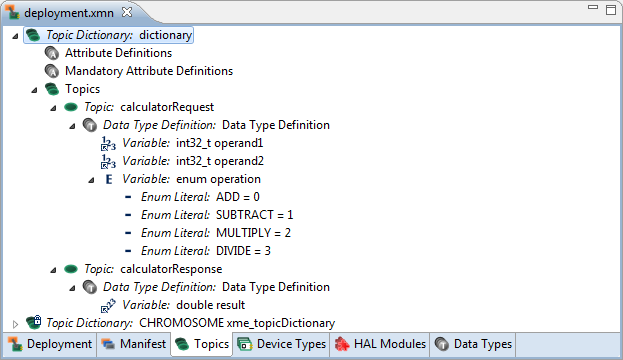
\includegraphics[scale=0.75]{figures/xmt_calculator_topics.png}
	\caption{Topic model of the \emph{calculator} example.}
	\label{fig:xmt_calculator_topics}
\end{figure}

Next, let's have a look at the component manifest of the \emph{calculator} example (compare Figure~\ref{fig:xmt_calculator_manifest}).
It lists two application-specific components:
\begin{itemize}
	\item A \emph{Calculator} component waits for client requests and handles them as they arrive.
		Furthermore, it provides respective output on the console.
	
	\item A \emph{Client} component sends a request using random numbers and operations and displays both request and response in its console.
\end{itemize}
%
\begin{figure}[htpb]
	\centering
	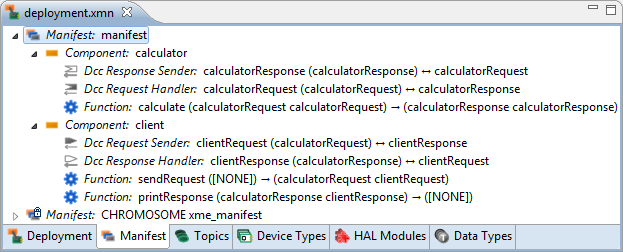
\includegraphics[scale=0.75]{figures/xmt_calculator_manifest.png}
	\caption{Component manifest of the \emph{calculator} example.}
	\label{fig:xmt_calculator_manifest}
\end{figure}
%
Using this simple setup, we can build a deployment model with three nodes as shown on Figure~\ref{fig:xmt_calculator_deployment}.
Notice that we instantiated the \emph{Client} component twice, both on \emph{client1Node} and on \emph{client2Node}.
This means that when we start the applications, requests will be sent to \emph{serverNode} from both client nodes,
but a response will only be delivered to the node that actually sent the request.
%
You might wonder why we need two client nodes. Could not we just launch the same compiled node twice?
Since the address of a node is hard-coded into its executable in this example, we cannot do that.
Otherwise, the server would be unable to distinguish between the two clients
and the used UDP port for communication would be already occupied by the other client process.

\begin{figure}[htpb]
	\centering
	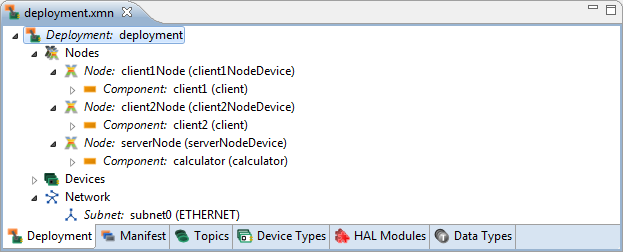
\includegraphics[scale=0.75]{figures/xmt_calculator_deployment.png}
	\caption{Deployment model of the \emph{calculator} example.}
	\label{fig:xmt_calculator_deployment}
\end{figure}

Now it's time to build the node files and run the example.
%
You should be able to build the nodes from within XMT by right-clicking on the root element in the deployment model and selecting \emph{Build Application...}.
In the build window, select the options according to Figure~\ref{fig:xmt_calculator_buildWindow}.
Notice that you need to setup the setting under \emph{Window} $\rightarrow$ \emph{Preferences} $\rightarrow$ \emph{XMT} $\rightarrow$ \emph{CMake}
correctly for this to work (using \emph{Visual Studio 10} as generator is recommended if you have Visual Studio 2010 installed).
Check the output in the XMT console window for any problems such as error messages.

\begin{figure}[htpb]
	\centering
	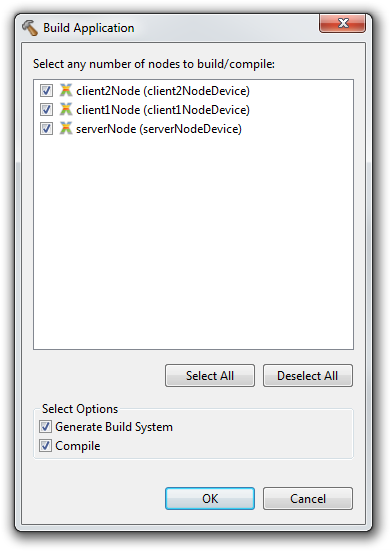
\includegraphics[scale=0.75]{figures/xmt_calculator_buildWindow.png}
	\caption{XMT build options for the \emph{calculator} example.}
	\label{fig:xmt_calculator_buildWindow}
\end{figure}

If this does not work as expected, follow the instructions from Section~\ref{sec:example_sensorMonitor:linux} (Linux)
or~\ref{sec:example_sensorMonitor:windows} (Windows) to manually create the build system and compile each of the three nodes
(\emph{serverNode}, \emph{client1Node} and \emph{client2Node}).

Now you can find the compiled executables in the following folders, where \texttt{<node>} is the name of the respective node:
\texttt{<XME\_ROOT>/examples/calculator/build/<node>/target/}.
%
On Windows, select the subfolder corresponding to the appropriate configuration name (usually \emph{Debug}).
You should find an executable in each of these folders, named like the node itself.
First run the \emph{serverNode} executable in order to start the calculator ``daemon''.
Subsequently, run \emph{client1Node} and \emph{client2Node} (in arbitrary order) to see them interact with the server.
The output should look similar to the one shown in Figures~\ref{fig:example_calculator_serverNode}, \ref{fig:example_calculator_client1Node}
and~\ref{fig:example_calculator_client2Node}.

Feel free to inspect the source code of the nodes, which you will find in the directory \texttt{<XME\_ROOT>/examples/calculator/src}.
The individual functions are implemented in the following files inside that directory:
\texttt{calculator/adv/client/src/sendRequestFunction.c} (\emph{sendRequest} function),
\texttt{calculator/adv/calculator/src/calculateFunction.c} (\emph{calculate} function) and
\texttt{calculator/adv/client/src/printResponseFunction.c} (\emph{printResponse} function).

\begin{figure}[htpb]
	\centering
	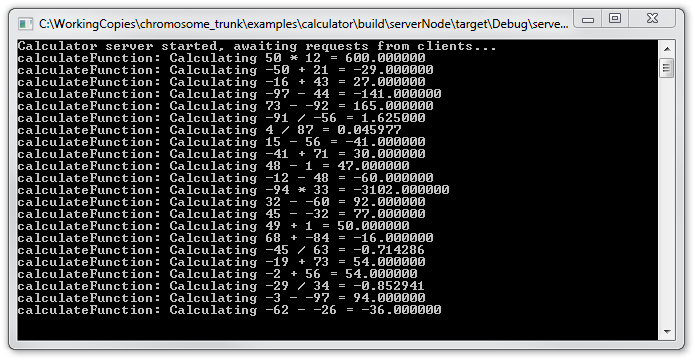
\includegraphics[scale=0.7]{figures/example_calculator_serverNode.png}
	\caption{Console window of \emph{serverNode}.}
	\label{fig:example_calculator_serverNode}
\end{figure}

\begin{figure}[htpb]
	\centering
	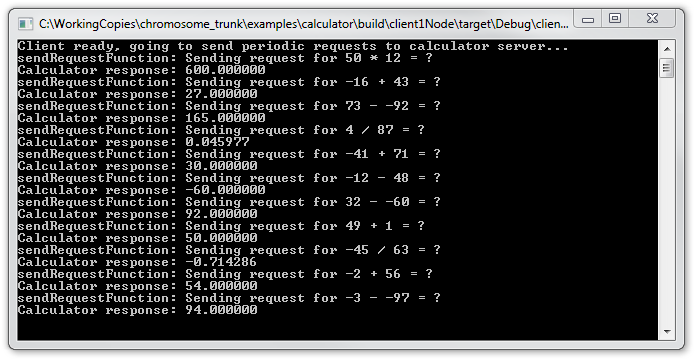
\includegraphics[scale=0.7]{figures/example_calculator_client1Node.png}
	\caption{Console window of \emph{client1Node}.}
	\label{fig:example_calculator_client1Node}
\end{figure}

\begin{figure}[htpb]
	\centering
	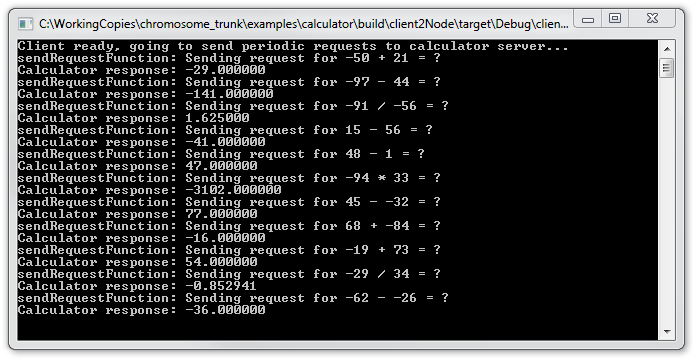
\includegraphics[scale=0.7]{figures/example_calculator_client2Node.png}
	\caption{Console window of \emph{client2Node}.}
	\label{fig:example_calculator_client2Node}
\end{figure}

\clearpage
%
% Copyright (c) 2011-2013, fortiss GmbH.
% Licensed under the Apache License, Version 2.0.
% 
% Use, modification and distribution are subject to the terms specified
% in the accompanying license file LICENSE.txt located at the root directory
% of this software distribution. A copy is available at
% http://chromosome.fortiss.org/.
%
% This file is part of CHROMOSOME.
%
% $Id$
%

% =================================================================
\section{Example 6: Consumer with Queue (10 minutes)}
\label{sec:example_queues}
% =================================================================

This is a simple example of queues used in a subscription.
To look at it, import the \textit{queues} example into XMT,
as you have previously done it with the \emph{sensorMonitor} example (see Section~\ref{sec:example_xmt}).

Queues on a subscription become necessary when multiple data items are sent to it,
before its function(s) can process the previous data item.
In this example there are two sender components and one receiver component on the same node.
Each sender component has a single publication, and each receiver has a subscription.
Therefore two local routes will be constructed that are connected to the subscription.
Each sender is executed at a frequency of 1.5~Hz, whereas the receiver is executed twice as often at a frequency of 3.0~Hz.
Therefore the receiver will in principle be executed often enough to consume all data items.
But it might happen that multiple data items arrive in the same cycle.
In this example the senders will each be executed in every other cycle,
so that two data items arrive at the receiver in that cycle.
The problem is that in a single cycle the receiver will only process a single data item.
To resolve this, the subscription of the receiver has its queue size set to \textit{2}, see screenshot~\ref{fig:example_queues_manifest}.
So in the subsequent cycle, the receiver will process the second data item (no new data items arrive),
which has been buffered in the queue.

\begin{figure}[htpb]
	\centering
	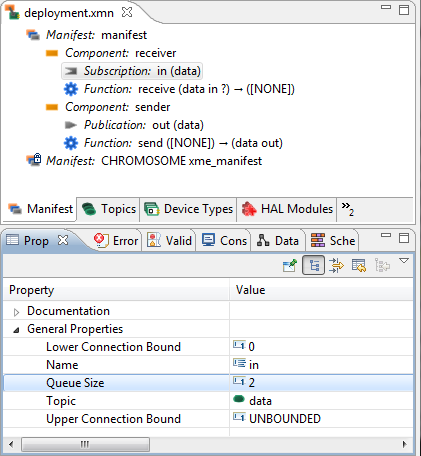
\includegraphics[scale=0.75]{figures/example_queues_manifest.png}
	\caption{Manifest of queues example, highlighting the queue size.}
	\label{fig:example_queues_manifest}
\end{figure}

Screenshot~\ref{fig:example_queues} shows the console output from the example.
On execution you will notice a 3 second delay between each receiver execution.
Despite two data items arriving at once it will be able to process both items.
Without a queue the second data item would have overwritten the first.

\begin{figure}[htpb]
	\centering
	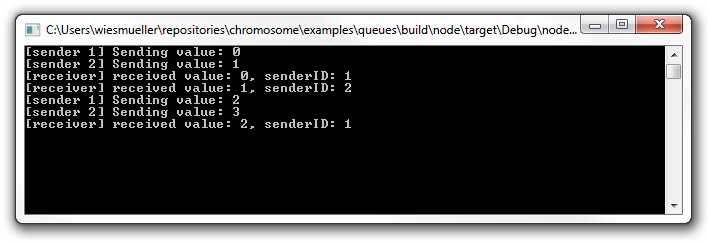
\includegraphics[scale=0.5]{figures/example_queues.png}
	\caption{Execution of queues example.}
	\label{fig:example_queues}
\end{figure}

\clearpage
%
% Copyright (c) 2011-2013, fortiss GmbH.
% Licensed under the Apache License, Version 2.0.
% 
% Use, modification and distribution are subject to the terms specified
% in the accompanying license file LICENSE.txt located at the root directory
% of this software distribution. A copy is available at
% http://chromosome.fortiss.org/.
%
% This file is part of CHROMOSOME.
%
% $Id$
%

% =================================================================
\section{Example 7: Configurator Extension (15 minutes)}
\label{sec:example_configuratorExtension}
% =================================================================

This examples shows the \textit{configurator extension} concept,
together with \textit{lower} and \textit{upper connection bounds} for input ports.
It is located in the directory \texttt{examples/configuratorExtension/}. 

The \textit{configurator extension} component of \xme allows to register configurators
that react on changes in the system configuration. Currently you can only
register configurators for the logical route graph.
After each change in the graph, for example after a plug~\&~play event, all
registered configurators will be called.
In the configurator you can inspect the current routes.
You can also add and remove\footnote{Not supported yet.} components, as
well as removing routes\footnote{Only supported for non-established routes.}.

\textit{Connection bounds} specify restrictions on the number of routes that an input
port is allowed to be connected to.
This is specified in the manifest of the component.
Currently this information is available at runtime~--~for example in a configurator~--~
but not enforced yet by \xme itself.

This example will register a configurator that uses the connection bound specification
and modifies the configuration accordingly.
Three nodes have been created for this showcase, see Figure~\ref{fig:example_configuratorExtension_deployment}.

\begin{figure}[htpb]
	\centering
	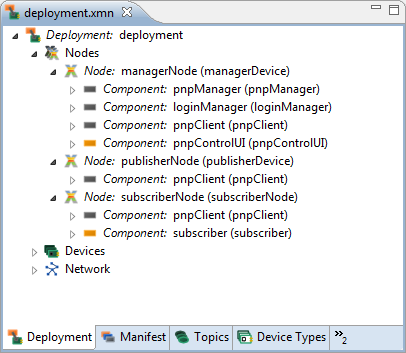
\includegraphics[scale=0.8]{figures/example_configuratorExtension_deployment.png}
	\caption{Deployment model of configurator extension example, showing all three nodes.}
	\label{fig:example_configuratorExtension_deployment}
\end{figure}

The \textit{subscriberNode} contains a single application-defined component of type \textit{subscriber}.
This component simply waits for data on its input port and prints it to the console.
When you navigate to the subscription of this component in its manifest~--~see Figure~\ref{fig:example_configuratorExtension_manifest}~--~%
you can see that it specifies a lower connection bound of $2$ and an upper connection
bound of $3$.

\begin{figure}[htpb]
	\centering
	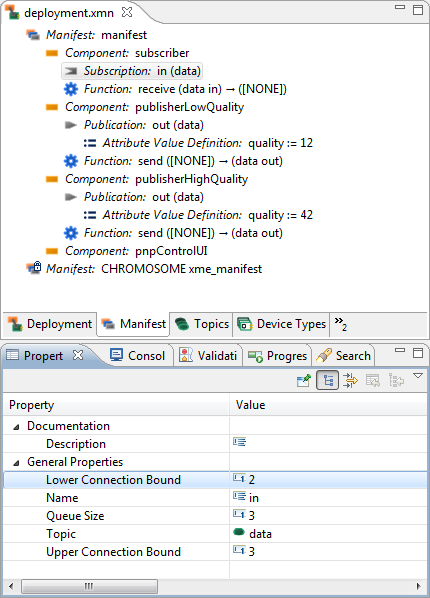
\includegraphics[scale=0.8]{figures/example_configuratorExtension_manifest.png}
	\caption{Manifest of configurator extension example.}
	\label{fig:example_configuratorExtension_manifest}
\end{figure}

The \textit{publisherNode} is initially empty except for the \textit{pnpClient}.
New components will be added to this node at runtime.

The component \textit{pnpControlUI} on the \textit{managerNode} will prompt the user
for plug \& play-related commands. We will use this interface to add new \textit{publisher}s.
There are two kinds of publishers, the \textit{lowQualityPublisher} and the \textit{highQualityPublisher}.
Both publish the same topic but assign different values to the \textit{quality} attribute.
Again you can have a look at these definition in the manifest, see Figure~\ref{fig:example_configuratorExtension_manifest}.

In this example a configurator is registered at the configurator extension.
See Listing~\ref{lst:configuratorExtensionRegistration} for the respective call in the \texttt{managerNode.c} file.
The implementation of the configurator can be found in the following directory:\newline
\texttt{src/configuratorExtension/configurator/demoConfigurator}.
%
The given configurator,
represented by the callback function \lstinline{configuratorExtension_configurator_demoConfigurator_callback()},
will perform the following two tasks:
%
\begin{enumerate}
	\item
		If any input port is connected to less routes than specified in its \textbf{lower connection bound},
		all routes from this port are removed.
		If a new component is to be created that does not satisfy the lower connection bound on one of its ports,
		component creation will be skipped.
	\item
		If any input port is connected to more routes than specified in its \textbf{upper connection bound},
		the excessive routes are removed. Routes with lower quality attribute values are removed first.
		A route with a topic that does not have this attribute is treated as having a quality value of $0$.
\end{enumerate}

\begin{quote}
\textbf{Note:} The removal of already established routes is currently not yet supported,
hence the routes of components that are already created will not be removed.
See Issue \#3952.
\end{quote}

%numbers=left,firstnumber=8842
\begin{lstlisting}[float,label={lst:configuratorExtensionRegistration},caption={Registration of configurator.},breaklines]
// PROTECTED REGION ID(MANAGERNODE_MAIN_RUN_BEFORE) ENABLED START

xme_core_pnp_configExt_addConfigurator
(
    XME_CORE_PNP_CONFIG_EXT_CONFIGURATORTYPE_LOGICAL_ROUTES,
    &configuratorExtension_configurator_demoConfigurator_callback,
    NULL
);

// PROTECTED REGION END
\end{lstlisting}

\noindent To see this behavior in action, run all three nodes and follow these instructions.
You may invoke the \texttt{list nodes} and \texttt{list types} commands to list active nodes and types, respectively.
(the numbers refer to the red numbers in Figure~\ref{fig:example_configuratorExtension_execution}).
\begin{enumerate}
	\item
		The managerNode asks you to enter a command.\newline
		Enter: \texttt{add 2 4100}\newline
		This will add a new component of type \textit{highQualityPublisher} (type ID \texttt{4100}) on the \textit{publisher} node (node ID \texttt{2}).
	\item
		The configurator informs you that the lower connection bound of the subscriber component is not satisfied.
		Therefore it removes the route and the component is not created yet (no output appears on the other nodes).
	\item
		Now enter: \texttt{add 2 4099}\newline
		This will add a new component of type \textit{lowQualityPublisher} (type ID \texttt{4099}) on the publisher node.
	\item
		Now the lower connection bound is satisfied and the new component is plugged.
		After waiting some time you will notice that both publishers start sending.
	\item
		Now enter: \texttt{add 2 4100}
	\item
		An additional \textit{highQualityPublisher} is added and will immediately be plugged in,
		as we now have three routes which is in the limits of the connection bounds of the subscriber.%
		\footnote{Currently having two instances of the same component type will lead to data loss.
		That is why you see a warning on the publisher node after instantiating the second \textit{highQualityPublisher}.
		See also known issue \#3964~\ref{appx:known_issues}.}
	\item
		When you subsequently enter: \texttt{add 2 4100}\newline
		The configurator will inform you that the maximum connection bound is exceeded and
		that it is going to remove the route of the \textit{lowQualityPublisher}.
		As previously noted, established routes cannot be removed yet, so the removal will not actually be executed.
\end{enumerate}

\begin{figure}[htpb]
	\centering
	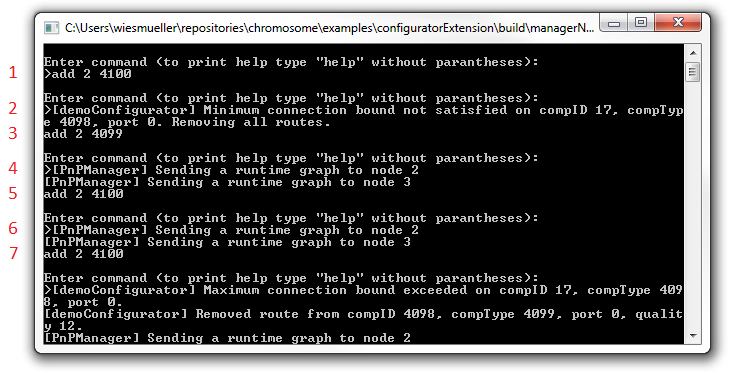
\includegraphics[scale=0.8]{figures/example_configuratorExtension_execution.png}
	\caption{Execution of configurator extension example.}
	\label{fig:example_configuratorExtension_execution}
\end{figure}

%\clearpage
%%
% Copyright (c) 2011-2013, fortiss GmbH.
% Licensed under the Apache License, Version 2.0.
% 
% Use, modification and distribution are subject to the terms specified
% in the accompanying license file LICENSE.txt located at the root directory
% of this software distribution. A copy is available at
% http://chromosome.fortiss.org/.
%
% This file is part of CHROMOSOME.
%
% $Id: example_chat.tex 7852 2014-03-14 16:32:01Z geisinger $
%

\section{Example 2: Chat with Chat Rooms (30 minutes)}
\label{sec:example_chat}

It is now time to replace the \emph{Hello World} application with a distributed \emph{Chat} application.
This tutorial comes with components that realize a distributed chat service.
The source code of this application is already present in the tutorial project,
we just need to configure it properly.

\begin{enumerate}
	\item The \emph{Hello World} application was using a specific component to print its ``\texttt{Hello World!}'' message.
		As this message is quite annoying in a chat room, we first have to remove the \emph{Hello World} component from the tutorial project.
		At the same time, we enable the \emph{Chat Component} which implements the chat client.
		This has to be done in the project's main file {\tt client.c},
		which can be opened in Visual Studio by double-clicking on the respective item
		below \emph{tutorial} $\rightarrow$ \emph{Source Files} in the \emph{Project Explorer} pane.
		Please comment the lines about the {\tt tutorial\_adv\_helloWorldComponent}
		and uncomment (enable) the lines about the {\tt tutorial\_adv\_chatComponent} as shown below:

\begin{lstlisting}[numbers=left,firstnumber=55,breaklines]

/* XME_COMPONENT_CONFIG_INSTANCE(tutorial_adv_helloWorldComponent, 1); */                                               /~~/ Comment the line above

XME_COMPONENT_CONFIG_INSTANCE(tutorial_adv_chatComponent, 1);                                             /~~/ Uncomment the line above

/*************************************************************************/
/***   Component descriptor                                            ***/
/*************************************************************************/
XME_COMPONENT_LIST_BEGIN
	XME_COMPONENT_LIST_ITEM(xme_core_nodeManager, 0)
	XME_COMPONENT_LIST_ITEM(xme_prim_ipLoginServerProxy, 0)
	XME_COMPONENT_LIST_ITEM(xme_prim_neighborhoodDiscovery, 0)
/*	XME_COMPONENT_LIST_ITEM(tutorial_adv_helloWorldComponent, 0)*/                                               /~~/ Comment the line above
	XME_COMPONENT_LIST_ITEM(tutorial_adv_chatComponent, 0)                                         /~~/ Uncomment the line above
XME_COMPONENT_LIST_END;
\end{lstlisting}

	\item The routing of messages is performed automatically by \xme core components.
		To keep the tutorial project small, all required components for network management and routing messages
		between distributed nodes (i.e., \emph{Login Server} and \emph{Master Directory}) have been added to a separate project named {\bf Coordinator}.
		We will treat the Coordinator as a separate node and have it running in the background so that people can dynamically enter chat rooms.
		
		To be able to use this functionality, please go go back to Section~\ref{sec:example_helloworld}
		and perform the described steps again for the \verb|coordinator| example.
		Please use the directory \verb|<XME_ROOT>/| \verb|examples/tutorial/application/coordinator| as input for the \emph{Where is the source code} field
		and use the directory \verb|<XME_ROOT>/examples/tutorial/build/coordinator| as input for the
		\emph{Where to build the binaries} field within CMake.
		After generation of the build system, the \verb|Coordinator.sln| Visual Studio solution file
		can be found in at \verb|<XME_ROOT>/examples/tutorial/build/coordinator|.
		Do not forget to set up \verb|coordinator| as the \emph{StartUp Project} within Visual Studio.
		
	\item After having successfully compiled the coordinator project as well as the tutorial project,
		a basic distributed chat application can be started.
		In order to do this, execute {\bf one instance} of the coordinator application.
		If you receive a request from the \emph{Windows Firewall},
		please allow communication to the \emph{Home or Company Network} as shown in Figure~\ref{fig:firewall_coordinator}.
		Note that if you have colleagues on the same network running this tutorial at the same time,
		you should talk to them to only run one instance of the Coordinator at any point in time.\footnote{%
			This is a limitation of the current version of \xme. We do not yet support multiple subnets
			or detect the presence of other Coordinator instances. This will change in future versions.}
		
		The Coordinator can either be started from Visual Studio or by executing \verb|<XME_ROOT>/|
		\verb|examples/tutorial/build/coordinator/target/*/coordinator.exe|.
		This will open a terminal window in which \xme may print logging information.
		By default, the log level is set up so that only warnings and errors will be shown,
		so it is normal for the terminal window to not show any activity.

\begin{figure}[htpb]
	\centering
	\includegraphics[scale=0.75]{figures/firewall_coordinator.png}
	\caption{Firewall settings for the \texttt{Coordinator} application.\TODO{Update image!}}
	\label{fig:firewall_coordinator}
\end{figure}

	\item We can now execute an arbitrary number of instances of the tutorial application.
		To do this, navigate to the respective directory and launch
		\verb|<XME_ROOT>/examples/tutorial/build| \verb|client/target/*/client.exe|.
		This will also open a terminal window, which first prompts to enter a name.
		After a name is given, you will be presented a list of commands and chat rooms to choose from
		(compare Figure~\ref{fig:example_chat}).

\begin{figure}[htpb]
	\centering
	\includegraphics[scale=0.75]{figures/example_chat.png}
	\caption{Sending chat messages via the \emph{Chat Component}.\TODO{Update image!}}
	\label{fig:example_chat}
\end{figure}

		The semantics of a chat room are that messages sent to a chat room should only be visible to people that have joined the respective chat room.
		This concept can be directly mapped to the notion of \emph{topics}.
		
		Anything that is not a command is interpreted as a message to send to the \emph{active} chat room.
		The active chat room can be changed with the \texttt{!s} command.
		
		Launch multiple instances of the chat example using different names and send some messages.
		Then run the application in a distributed way using multiple computers on the same subnet.

\end{enumerate}

%\clearpage
%%
% Copyright (c) 2011-2013, fortiss GmbH.
% Licensed under the Apache License, Version 2.0.
% 
% Use, modification and distribution are subject to the terms specified
% in the accompanying license file LICENSE.txt located at the root directory
% of this software distribution. A copy is available at
% http://chromosome.fortiss.org/.
%
% This file is part of CHROMOSOME.
%
% $Id: example_chatcalculator.tex 7852 2014-03-14 16:32:01Z geisinger $
%

\section{Example 3: Chat Calculator (20+ minutes)}
\label{sec:example_chatcalculator}

After having modified an already existing component in Section~\ref{sec:example_chat},
it is now time to create a completely new component.
%
A so-called \emph{Chat Calculator} component is a good starting point for digging deeper into \xme.
%
The calculator should fulfill the following requirements:
\begin{itemize}
	\item Join a chat room.
	\item Announce its presence in the chat room every 30 seconds.
	\item Listen to commands of the form ``\verb|!calc <operand1> <operation> <operand2>|''.
	\item Support addition, subtraction, multiplication and divison as \verb|<operation>|.
	\item Send calculated results to the chat room in the form\\
		``\verb|<operand1> <operation> <operand2> = <result>|''.
	\item Gracefully handle division by zero.
\end{itemize}

The following steps guide you through the implementation of the \emph{Calculator Component}.
Please be warned that the given time frame of 20 minutes does not include thorough reading and understanding of the code.
You can find electronic versions of the code for the \emph{Calculator Component} on the \xme website\footnote{%
\url{http://chromosome.fortiss.org/}}.

\begin{enumerate}
	\item Use the \emph{Template Generator} application to create a new component with name ``\texttt{Chat Calculator}'' of class \verb|adv| (advanced).
		The \emph{Template Generator} application can be found in the directory \verb|<XME_ROOT>/../bin/windows_x86| and is explained in FAQ~\ref{faq:create_component}.
		
		The application will generate two files named \verb|chatCalculator.h| and \verb|chatCalculator.c|
		in the directory \verb|<XME_ROOT>/examples/tutorial/tutorial/adv| and fill it with sample content.
		Furthermore, it will automatically add the new component to the \verb|CMakeLists.txt| file in the same directory.
		This is the quickest way to generate a new \xme component.

%	\item First, we need to decide whether the new component will be a member of the class \texttt{adv} (advanced),
%		\texttt{prim} (primitive) or \texttt{hal} (hardware abstraction).
%		These classes define how the component can communicate with other components.
%		Application components like the \emph{Calculator Component} are typically \emph{advanced},
%		which means that they can exchange data with other application components only using data centric communication.
%		We choose \verb|tutorial_adv_chatCalculator| as our component name.
%
%	\item Create a C source and header file in the coresponding folder \verb|<XME_ROOT>/| \verb|examples/tutorial/tutorial/adv|,
%		and name it \verb|tutorial_|\textsf{\itshape class}\verb|_|\textsf{\itshape name}, where \textsf{\itshape name} is the name of the component,
%		preferably in \texttt{camelCaseWriting} style if the name consists of multiple words.

%	\item In the folder where the new header and source file is located,
%		edit \verb|CMakeLists.txt| and insert the new component into the list:
%
%\begin{lstlisting}[numbers=left,firstnumber=18]
%xme_add_component(   # Add this block
%	"tutorial_adv_chatCalculator"
%	tutorial_adv_chatCalculator.h tutorial_adv_chatCalculator.c
%)
%\end{lstlisting}

	\item Edit the \verb|CMakeLists.txt| file of the \verb|<XME_ROOT>/examples/tutorial/application/client| project to use the new component:

\begin{lstlisting}[language=cmake,numbers=left,firstnumber=62]
# Build XME components
xme_link_components(
	"client"
	xme_core_core
	xme_prim_ipLoginServerProxy
	xme_hal_net
	xme_hal_sleep
	tutorial_adv_chatCalculator   ~\char"0023~ Add this line
)
\end{lstlisting}

		Note that CMake will automatically pick up the changes in \verb|CMakeLists.txt| when we perform the next full compile.
		This is why you do not have to rerun CMake manually after this change.

	\item Open the \verb|Client| solution with the modifications from Section~\ref{sec:example_chat} in \emph{Visual Studio}
		and edit \verb|client.c| to include the new component:

	\begin{lstlisting}[numbers=left,firstnumber=25]
/*************************************************************************/
/***   Includes                                                        ***/
/*************************************************************************/
#include "tutorial/adv/chatComponent.h"
#include "tutorial/adv/helloWorldComponent.h"
#include "xme/core/componentList.h"
#include "xme/prim/ipLoginServerProxy.h"
#include "tutorial/adv/chatCalculator.h"   /~~/ Add this line
\end{lstlisting}

	\item Declare the component configuration and add an instance of the component
		to the component list in \verb|client.c|. Apply the following two modifications:

\begin{lstlisting}[numbers=left,firstnumber=35,breaklines]
/*************************************************************************/
/***   Component configurations                                        ***/
/*************************************************************************/
XME_COMPONENT_CONFIG_INSTANCE(xme_core_nodeManager) =
{
	0x00000000021041A1, // deviceType
	XME_CORE_DEVICE_GUID_RANDOM // deviceGuid
};

XME_COMPONENT_CONFIG_INSTANCE(xme_prim_ipLoginServerProxy, 1);

XME_COMPONENT_CONFIG_INSTANCE(xme_prim_neighborhoodDiscovery) =
{
	{
		(xme_hal_time_timeInterval_t)1000000000, // announcementInterval
		(xme_core_dataChannel_t)302, // dataChannelForAnnouncements
		5 // ticksBeforeRemovingReceivedAnnouncements
	}
};

/* XME_COMPONENT_CONFIG_INSTANCE(tutorial_adv_helloWorldComponent, 1); */

XME_COMPONENT_CONFIG_INSTANCE(tutorial_adv_chatComponent, 1);

XME_COMPONENT_CONFIG_INSTANCE(tutorial_adv_chatCalculator) =
{                                                        /~~/ Add this block
	{
		// public
		CHAT_TOPIC_BASE // topic
	}
};

/*************************************************************************/
/***   Component descriptor                                            ***/
/*************************************************************************/
XME_COMPONENT_LIST_BEGIN
	XME_COMPONENT_LIST_ITEM(xme_core_nodeManager, 0)
	XME_COMPONENT_LIST_ITEM(xme_prim_ipLoginServerProxy, 0)
	XME_COMPONENT_LIST_ITEM(xme_prim_neighborhoodDiscovery, 0)
/*	XME_COMPONENT_LIST_ITEM(tutorial_adv_helloWorldComponent, 0) */
	XME_COMPONENT_LIST_ITEM(tutorial_adv_chatComponent, 0)
	XME_COMPONENT_LIST_ITEM(tutorial_adv_chatCalculator, 0)                                               /~~/ Add the line above
XME_COMPONENT_LIST_END;
\end{lstlisting}

	\item After these changes, press \emph{F7} in \emph{Visual Studio} to build the solution.
		This is required for CMake to pick up the changes in the build system.
		You will probably notice CMake re-run automatically in the \emph{Visual Studio} console.
		You might be prompted whether to reload the \emph{Visual Studio Solution}, in which case you should choose \emph{Reload}
		(compare Figure~\ref{fig:vs_detect_change_tutorial}).

\begin{figure}[htpb]
	\centering
	\includegraphics[scale=0.75]{figures/vs_detect_change_tutorial.png}
	\caption{\emph{Visual Studio Solution} reload prompt after \emph{CMake} has regenerated the build system.\TODO{Update image!}}
	\label{fig:vs_detect_change_tutorial}
\end{figure}

	\item You should now see the \verb|tutorial_adv_chatCalculator| item in the \emph{Project Navigator} pane in \emph{Visual Studio}.
		You can comfortably edit the source and header file of the component from there.

\begin{figure}[htpb]
	\centering
	\includegraphics[width=\textwidth]{figures/vs_chatCalculator.png}
	\caption{\texttt{tutorial\_adv\_chatCalculator} component in the \emph{Visual Studio Project Navigator} pane.\TODO{Update image!}}
	\label{fig:vs_chatCalculator}
\end{figure}

	\item The component we have just added comes with some example code that we have to adapt in order to implement the \emph{Chat Calculator}.
		Open the respective files \verb|chatCalculator.h| and \verb|chatCalculator.c| found in \verb|<XME_ROOT>/examples/tutorial/tutorial/adv| to make yourself familiar with the generated code.
		You will notice that the generated example code publishes and subscribes the \verb|XME_CORE_TOPIC_EVENT| topic
		and that a task is created that prints a message every two seconds.
		The publication and subscription handles as well as the task handle is stored in the component's configuration structure \verb|tutorial_adv_chatCalculator_configStruct_t|.
		
		We can reuse the existing functionality for implementing the \emph{Chat Calculator},
		because the calculator has to listen (read: subscribe) to a specific chat room
		and print (read: publish) the result of the calculation.
		Furthermore, we need to announce the presence of the \emph{Chat Calculator} every 30~seconds,
		for which the task can be used.
		
		In order to ensure maximum flexibility (and to demonstrate how to use configuration variables),
		we will configure the topic of the chat room to enter (i.e., the topic) in \emph{Chat Calculator}'s configuration.
		For this, we will define a member variable called \verb|topic| in the comfiguration structure
		that we can set to an arbitrary value in our main program when we instantiate the component.
		In \verb|chatCalculator.h|, apply the following two changes:

\begin{lstlisting}[numbers=left,firstnumber=33]
/*************************************************************************/
/***   Type definitions                                                ***/
/*************************************************************************/
typedef struct
{
	// public
	xme_core_topic_t topic;                             /~~/ Change this line
	// private
/*	int dummyState; */                       /~~/ Comment or remove this line
	xme_core_resourceManager_taskHandle_t taskHandle;
	xme_core_dcc_publicationHandle_t publicationHandle;
	xme_core_dcc_subscriptionHandle_t subscriptionHandle;
}
tutorial_adv_chatCalculator_configStruct_t;
\end{lstlisting}

		We can leave the rest of the header file as-is.

	\item Now it is time to implement the actual functionality in \verb|chatCalculator.c|.
		Start by changing the published and subscribed topic to the chat room in which we want the \emph{Chat Calculator} to be.
		Apply the following four changes:

\begin{lstlisting}[numbers=left,firstnumber=69]
xme_core_status_t
tutorial_adv_chatCalculator_create(tutorial_adv_chatCalculator_configStruct_t* config)
{
	// TODO: Initialize component state
/*	config->dummyState = 0; */               /~~/ Comment or remove this line

/*	// TODO: Add code */                    /~~/ Comment or remove this block
//	XME_LOG(XME_LOG_NOTE, "Create function of Chat Calculator called!\n");

	// Example: Publish a topic
	config->publicationHandle =
		xme_core_dcc_publishTopic
		(
			config->topic,                              /~~/ Change this line
			XME_CORE_MD_EMPTY_META_DATA,
			false,
			NULL
		);

	// Check for errors
	if (XME_CORE_DCC_INVALID_PUBLICATION_HANDLE == ~\LstSuppressNumber~
		                                         config->publicationHandle) ~\LstReactivateNumber~
	{
		return XME_CORE_STATUS_INTERNAL_ERROR;
	}

	// Example: Subscribe to a topic
	config->subscriptionHandle =
		xme_core_dcc_subscribeTopic
		(
			config->topic,                              /~~/ Change this line
			XME_CORE_MD_EMPTY_META_DATA,
			false,
			_tutorial_adv_chatCalculator_receiveDataCallback,
			config
		); ~\LstSuppressNumber~

	[...]                           /~~/ Leave the rest of the function as-is
} ~\LstReactivateNumber~
\end{lstlisting}

	\item Now we should adapt the \verb|_tutorial_adv_chatCalculator_receiveDataCallback()| function,
		which handles incoming data for the subscribed topic:

\begin{lstlisting}[numbers=left,firstnumber=28,breaklines]
/*************************************************************************/
/***   Implementation                                                  ***/
/*************************************************************************/
// TODO: Use or remove this sample topic subscription callback function:
static
void
_tutorial_adv_chatCalculator_receiveDataCallback(xme_hal_sharedPtr_t dataHandle, void* userData)
{
	// TODO: In case you supply the component's configuration instance
	//       via userData when subscribing, you can access it here:
	tutorial_adv_chatCalculator_configStruct_t* config = ~\LstSuppressNumber~
                     (tutorial_adv_chatCalculator_configStruct_t*)userData; ~\LstReactivateNumber~

/*	// TODO: Add code */                    /~~/ Comment or remove this block
//	XME_LOG(XME_LOG_NOTE, "Receive data callback function called!\n");
	
/*	// Example: Print data to screen */     /~~/ Comment or remove this block
//	{
//		const char* message = xme_hal_sharedPtr_getPointer(dataHandle);
//		XME_LOG(XME_LOG_NOTE, "Received: %s\n", message);
//	}

	/~~/ Add all the following lines

	char* input = (char*)xme_hal_sharedPtr_getPointer(dataHandle);
	int size = xme_hal_sharedPtr_getSize(dataHandle);

	// Output data
	char output[512];

	// Sanitize input
	input[size-1] = 0;

	// Strip person's name
	input = strchr(input, ':');
	if (NULL == input)
	{
		// Invalid message format
		return;
	}
	input += 2;

	if (0 != strncmp(input, "!calc ", 6))
	{
		// Not a calculation command
		return;
	}

	_tutorial_adv_chatCalculator_getResultString
	(
		input, output, sizeof(output)
	);

	if (0 != strlen(output))
	{
		xme_core_dcc_sendTopicData
		(
			config->publicationHandle,
			(void*)output, strlen(output)+1
		);
	}
}
\end{lstlisting}

	\item Add the \verb|_tutorial_adv_chatCalculator_getResultString()| function, which calculates the result of an operation,
		above \verb|_tutorial_adv_chatCalculator_receiveDataCallback()|:

\begin{lstlisting}[numbers=left,firstnumber=31]
static
void
_tutorial_adv_chatCalculator_getResultString(char* in, char* out, int outSize)
{
	// Error messages
	const char* error_syntax = "The expression could not be evaluated";
	const char* error_zero = "Division by zero";
	const char* error_op = "Invalid operator";

	double operand1, operand2, result;
	char op;
	char* pos;

	// Parse string
	pos = strchr(in, 0x20);
	if (NULL == pos)
	{
		strcpy_s(out, outSize, error_syntax);
		return;
	}
	operand1 = atof(pos+1);

	pos = strchr(pos+1, 0x20);
	if (NULL == pos)
	{
		strcpy_s(out, outSize, error_syntax);
		return;
	}
	op = *(pos+1);
	
	// Ignore own announcement message
	if ('<' == op)
	{
		out[0] = 0;
		return;
	}

	pos = strchr(pos+1, 0x20);
	if (NULL == pos)
	{
		strcpy_s(out, outSize, error_syntax);
		return;
	}
	operand2 = atof(pos+1);

	// Check for operator and division by zero
	if (!_tutorial_adv_chatCalculator_isOperationValid(op))
	{
		strcpy_s(out, outSize, error_op);
		return;
	}
	if (_tutorial_adv_chatCalculator_isDivisionByZero(op, operand2))
	{
		strcpy_s(out, outSize, error_zero);
		return;
	}

	// Calculate result
	result =
		_tutorial_adv_chatCalculator_calculateResult(operand1, op, operand2);

	// Output result
	xme_hal_safeString_snprintf
	(
		out, outSize, "%lf %c %lf = %lf",
		operand1, op, operand2, result
	);
}
\end{lstlisting}

	\item Add the following three includes to \verb|chatCalculator.c|:
	
\begin{lstlisting}[numbers=left,firstnumber=23]
/*************************************************************************/
/***   Includes                                                        ***/
/*************************************************************************/
#include "xme/adv/chatCalculator.h"

#include "xme/hal/safeString.h"                            /~~/ Add this line

#include <~\texttt{float}~.h>                                          /~~/ Add this line
#include <math.h>                                          /~~/ Add this line
\end{lstlisting}

	\item Add the following helper functions above \verb|_tutorial_adv_chatCalculator_getResultString()|:

\begin{lstlisting}[numbers=left,firstnumber=36]
static
bool
_tutorial_adv_chatCalculator_isOperationValid(char operation)
{
	return ('+' == operation || '-' == operation ||
		'/' == operation || '*' == operation);
}

static
bool
_tutorial_adv_chatCalculator_isDivisionByZero(char operation, double operand2)
{
	return ('/' == operation && fabs(operand2) < DBL_EPSILON);
}

static
double
_tutorial_adv_chatCalculator_calculateResult(double operand1, char operation,
                                                         double operand2)
{
	if ('+' == operation)
	{
		return operand1 + operand2;
	}
	if ('-' == operation)
	{
		return operand1 - operand2;
	}
	if ('*' == operation)
	{
		return operand1 * operand2;
	}
	if ('/' == operation)
	{
		// Division by zero is handled in isDivisionByZero()
		return operand1 / operand2;
	}

	// Invalid operation is handled in isOperationValid()
	return 0;
}
\end{lstlisting}

	\item Change the text the task sends to the chat room and remove debug output:

\begin{lstlisting}[numbers=left,firstnumber=207]
// TODO: Use or remove this sample task callback function:
static
void
_tutorial_adv_chatCalculator_taskCallback(void* userData)
{
	// TODO: In case you supply the component's configuration instance
	//       via userData when creating the task, you can access it here:
	tutorial_adv_chatCalculator_configStruct_t* config = ~\LstSuppressNumber~
                          (tutorial_adv_chatCalculator_configStruct_t*)userData; ~\LstReactivateNumber~

/*	// TODO: Add code */                    /~~/ Comment or remove this block
//	XME_LOG(XME_LOG_NOTE, "Task callback function called!\n");

	// Example: Send data
	{                                         /~~/ Change the following lines
		static const char* message = "Chat Calculator awaiting commands.\n"
			"Usage: !calc <operand1> <operation> <operand2>"; ~\LstSuppressNumber~
		[...]                       /~~/ Leave the rest of the function as-is
	}
} ~\LstReactivateNumber~
\end{lstlisting}

	\item Configure the task to fire every 30 seconds instead of every two seconds
		and remove debug output:

\begin{lstlisting}[numbers=left,firstnumber=274]
xme_core_status_t
tutorial_adv_chatCalculator_activate(tutorial_adv_chatCalculator_configStruct_t* config)
{
/*	// TODO: Add code */                    /~~/ Comment or remove this block
//	XME_LOG(XME_LOG_NOTE, "Activate function of Chat Calculator called!\n");

	// Example: Start a task:
	config->taskHandle =
		xme_core_resourceManager_scheduleTask
		(
			1000,
			30000,                                      /~~/ Change this line
			XME_HAL_SCHED_PRIORITY_NORMAL,
			_tutorial_adv_chatCalculator_taskCallback,
			config
		); ~\LstSuppressNumber~

	[...]                           /~~/ Leave the rest of the function as-is
} ~\LstReactivateNumber~
\end{lstlisting}

	\item Finally, remove some more debug output:

\begin{lstlisting}[numbers=left,firstnumber=300]
void
tutorial_adv_chatCalculator_deactivate(tutorial_adv_chatCalculator_configStruct_t* config)
{
/*	// TODO: Add code */                    /~~/ Comment or remove this block
//	XME_LOG(XME_LOG_NOTE, "Deactivate function of Chat Calculator called!\n"); ~\LstSuppressNumber~

	[...]                           /~~/ Leave the rest of the function as-is
} ~\LstReactivateNumber~
\end{lstlisting}

\begin{lstlisting}[numbers=left,firstnumber=310]
void
tutorial_adv_chatCalculator_destroy(tutorial_adv_chatCalculator_configStruct_t* config)
{
/*	// TODO: Add code */                    /~~/ Comment or remove this block
//	XME_LOG(XME_LOG_NOTE, "Destroy function of Chat Calculator called!\n"); ~\LstSuppressNumber~

	[...]                           /~~/ Leave the rest of the function as-is
} ~\LstReactivateNumber~
\end{lstlisting}

	\item Since we included the file \verb|xme/hal/safeString.h|, we also have to link against the respective component.
		We should specify that fact by adding a dependency to our \emph{Chat Calculator} component.
		Open \verb|tutorial/adv/CMakeLists.txt| and add the following line:

\begin{lstlisting}[language=cmake,numbers=none]
xme_add_component (
	"tutorial_adv_chatCalculator"
	chatCalculator.h chatCalculator.c
	xme_hal_safeString                                     /~~/ Add this line
)
\end{lstlisting}

	\item That's it! Compile and run the \verb|client| example (press \emph{F7} and \emph{F5} in \emph{Visual Studio}).
		Test the new component by letting the \emph{Chat Calculator} do your math homework ;)
\end{enumerate}

\section{More Examples}

You might consider implementing the following components to get to know \xme even better:
\begin{itemize}
	\item A ``spammer'' component that sends unsolicited advertisements to chat channels.
	\item A component that keeps track of all persons in each chat room and supports a ``\verb|!who|'' command to print a list
		(you might want to extend the \emph{Chat Example} to publish additional data in order to do this).
	\item A ``lunch time'' component that announces lunch time at noon in every chat room.
\end{itemize}

%\section{Questions to Reviewers}
%\begin{enumerate}
%	\item Did you encounter any inconsistencies between this tutorial and the actual source code?
%	\item Did you get enough/the right information from Sec. \ref{sec:architecture} (''XME in a Nutshell'')?
%	\item Did you encounter any other \emph{noticeable} situations, while working through this tutorial?
%\end{enumerate}

\clearpage
\appendix

%
% Copyright (c) 2011-2013, fortiss GmbH.
% Licensed under the Apache License, Version 2.0.
% 
% Use, modification and distribution are subject to the terms specified
% in the accompanying license file LICENSE.txt located at the root directory
% of this software distribution. A copy is available at
% http://chromosome.fortiss.org/.
%
% This file is part of CHROMOSOME.
%
% $Id$
%

\section{Known Issues}
\label{appx:known_issues}

The following known issues exist in this release.
They will be fixed in upcoming releases.

\subsection{Issue \#2968: XMT: Data sinks not scheduled multiple times for multiple incoming data stream}

Code generated from XMT has the same issue than described in \#2967.

\subsection{Issue \#3039: Separate the various XME applications in the same network from each other}

As soon as multiple XME ''master'' nodes (nodes with \emph{Login Managers}) run in the same network
(e.g., during testing of various applications) at the same time, XME will be come nondeterministic.
The reason for this is that a client will connect to any available master and it can not be guaranteed
that all nodes of an application will belong to the same XME network.

As a simple solution we could include the same GUID into all nodes belonging to the same network.
If the GUID is zero, it will be have like now. A client will connect to the first master available.
But it the GUID is not zero, a client will only connect to the master carrying the same GUID.

\subsection{Issue \#3076: Decide upon action if a function exceeds its timeslice in the schedule}

Currently, a function can block the execution of other functions:
if a function overshoots its worst case execution time (WCET), currently no action is taken.
This means that the other function following the ''blocker'' in the schedule will be delayed.
When the ''blocker'' finally ends, the other functions will be repeatedly executed in quick succession until the delay is compensated.

\subsection{Issue \#3183: Monitor losing data}

When sensor and empty nodes are running together the monitor node loses data. So we do not see all updates sent by the nodes on Monitor console.

The reason for this is that data gets internally overwritten on the receiver side if more data gets received than can be handled within one cycle of execution.
Queues have been recently introduced to cope with this problem, but configuration of the queue size is still a manual task
(can be performed in XMT, see \emph{queues} example for illustration).
It is planned to automatically calculate the required queue size based on a specification of the expected input behavior.

\subsection{Issue \#3374: Compiler warnings when building under Visual Studio 2012}

\texttt{warning C28251: Inconsistent annotation for '...': this instance has no\\
annotations. See ...}

\subsection{Issue \#3514: Scheduling algorithm to address the duration/frequency of functions additional to WCET}

With this feature the scheduling principle in the \emph{Plug and Play Client} for the components received in the runtime graph have to be modified.
This also may apply to the data structure of runtime graph which is communicated across from \emph{Plug and Play Manager} to \emph{Plug and Play Client}.

\subsection{Issue \#3548: Support for multiple request/response relationships per component}

The \emph{Logical Route Manager} is currently unable to correctly handle multiple request/response communication relationships in a single component.
The reason for this is that if multiple request or response ports exist, the LRM is unable to determine which request port belongs to which response port.

Consider the example of a ''server'' component with two request handler ports and two response sender ports with different request and response topics.
In this case, channel mappings might get generated from both input ports to both output ports, which is not the intended behavior.
In order to resolve this problem, we need to:
\begin{itemize}
	\item Either introduce a relationship between input port and output port (index) for every pair of request and response ports.
	\item Or derive the information from the dependency of the associated functions, if possible.
		This would require that functions are uniquely associated with at most one request and one response port.
		However, this is probably not meaningful, because the execution semantics of request sending functions
		and response handling functions is different and hence one might want to put them into two separate functions.
\end{itemize}

\subsection{Issue \#3683: ``Generate Build System'' of ``Build Application...'' in deployment model does not work under Linux}

When triggering the action commands are executed, but the build system is not generated. It seems that there are ``''-marks missing surrounding the cmake call with path and the \texttt{-G} option.

\subsection{Issue \#3727: Instantiating same component type twice at runtime causes error}

Calling \texttt{xme\_core\_pnp\_pnpClient\_instantiateComponentOnThisNode()} twice on a node for the same component type fails.

\subsection{Issue \#7344: Input port used by multiple functions leads to nondeterministic behavior}

This leads to undeterministic behaviour. Only one of the functins (``randomly'' chosen depending on the currentl slot in the Execution Manager) will actually process data on the input port.
The first function calls completeReadOperation on that port, so that the other function(s) do(es) not receive the data.

\subsection{Issue \#3779: pnpInit in \texttt{<node>.c} does not work if node contains \{pnp, login\}\{Client, Master\}}

If the node identifier of \texttt{xme\_core\_pnp\_pnpManager\_instantiateComponentOnNode()} in \texttt{pnpInit} of \texttt{<node>.c} is 0 (dynamic case), you receive the following run-time error:

\begin{verbatim}
xme_core_pnp_pnpManager_instantiateComponentOnNode component failed.
Fatal: Error occurred during initialization of CHROMOSOME pnp components.
Aborting execution.
\end{verbatim}

\subsection{Issue \#3833: Data structures not completely freed after the required components are removed}

Consider the following scenario:
Node A : running pnpManager (\emph{Plug and Play Manager})
Node B : running pnpClient (\emph{Plug and Play Client}), sensorComponent in that order in the schedule
Node C : running pnpClient (\emph{Plug and Play Client}), monitorComponent in that order in the schedule
Node B and C have a route between sensorComponent and monitorComponent.

Node B is logged out, Node A sends respective graphs to Node B and Node C.
Node B shuts down XME.
For Node C, pnpClient deletes the function descriptor of monitorComponent and removes the monitorComponent from schedule. The new schedule gets only activated from the next cycle.
Since monitorNode is run after the pnpClient in the current active schedule, if we delete the function descriptor this causes EM to see a fault and it issues a shutdown of the node C.
This is not correct.
Hence currently XME does not free the data structures. This is a memory leak.

\subsection{Issue \#3834: Nodes can only be logged out one at a time}

Currently we can logout one node in one execution cycle.
If multiple nodes are submitted for logout only the last one will be logged out. Request for the rest will be overwritten.

\subsection{Issue \#3836: Incorrect stop semantics may lead to loss of data}

Currently after we receive a logout or stop a component request, XME simply tries to take he required action as soon as possible.
This may result in loss of data, if there is any, in the ports of the components.
This may be undesirable in certain cases and one must have some policies regarding the same.
This becomes even more important when we have queues.

\subsection{Issue \#3848: \texttt{XME\_ASSERT\_NORVAL} in configureSchedule of \texttt{<node>.cpp} raises unexpected exception in C++ mode under MSVC}

For the \texttt{XME\_ASSERT\_NORVAL}s in \texttt{configureSchedule()} of the node files the warning C4297 is raised if compiling in C++ mode.

\subsection{Issue \#3964: Schedule output-related waypoints immediately after associated component}

Currently component instances of the same type share their ports.
The schedule calculation at runtime does not take this into account.
This leads to each component instance overwriting the data of the one scheduled before it.
On the console this triggers a warning of data loss.

\subsection{Issue \#4205: Overwriting of master CMakeLists.txt when using more than one deployment model}

When using more than one deployment model, regeneration of files leads to overwriting of master \texttt{CMakeLists.txt} in application root directory.

\subsection{Issue \#4262: When calling logout of a node the node shall be stopped}

If a node has logged in before, but the manager node vanished in the meantime,
a logout request sent by the node will timeout and the node will never shut down.

\clearpage
%
% Copyright (c) 2011-2013, fortiss GmbH.
% Licensed under the Apache License, Version 2.0.
% 
% Use, modification and distribution are subject to the terms specified
% in the accompanying license file LICENSE.txt located at the root directory
% of this software distribution. A copy is available at
% http://chromosome.fortiss.org/.
%
% This file is part of CHROMOSOME.
%
% $Id: faq.tex 7852 2014-03-14 16:32:01Z geisinger $
%

\section{Frequently Asked Questions}
\label{appx:faq}

\subsection{Organizational Questions}

\subsubsection{What is the \xme roadmap/release plan?}

See Appendix~\ref{appx:roadmap}.

\subsubsection{Can I use \xme in commercial software?}

Yes. Our licensing conditions allow this (see Appendix~\ref{appx:license}).
Notice however that the software is provided ''as-is''.

\subsubsection{Can I contribute?}

Yes. In case you are interested in contributing the \xme code base, let us know.
Find contact information on the first page of this document.

\subsection{Technical Questions}

%\subsubsection{How can I create a new component?}
%\label{faq:create_component}
%
%\xme comes with an application that can create template files for new components.
%This application is called \verb|templateGenerator| and can be found in the \verb|bin/windows_x86|
%subdirectory of the release package or built manually just like any other \xme example program (see Section~\ref{sec:example_helloworld} for hints).
%
%The application will ask you for the component name, type as well as your name (for the author field)
%and generate a header and a source file for the new component in the respective directory (compare Figure~\ref{fig:example_templateGenerator}).
%Consider using one of the existing example applications for testing your new component if application, see Section~\ref{sec:example_chatcalculator}
%for more information on how to embed a new component into an existing application.
%
%\begin{figure}[htbp]
	%\centering
	%\includegraphics[scale=0.75]{figures/example_templateGenerator.png}
	%\caption{\emph{Template Generator} in action.}
	%\label{fig:example_templateGenerator}
%\end{figure}
%
%\subsubsection{How can I define a new topic?}
%
%Topic identifiers are simple numbers with associated semantics.
%The \verb|xme_core_topic_t| type defined in file \verb|<XME_ROOT>/xme/core/topic.h| declares some generic topic identifiers.
%Topic numbers in the range between zero and \verb|XME_CORE_TOPIC_USER|-1 are reserved for internal use.
%This means that you can define a new topic by using an arbitrary number larger or equal to \verb|XME_CORE_TOPIC_USER|.
%
%Note that there is currently no mechanism in place for checking that the same topic identifiers are always used for the same type of data.
%Be aware that other people in the same network might use the same topic identifiers for their data.
%We plan to put a mechanism in place for avoiding this issue in future versions of \xme.

\subsubsection{How can I port \xme to my own target platform?}

The current release of \xme supports only Linux and Windows.
However, we are in the process of developing platform support layers for other platforms.
These include, for example, medium-sized microcontroller platforms like ARM Cortex M3 (e.g., as central control units).
Upcoming releases of \xme will ship with the respective functionality.
Let us know if you are interested in these topics.

If you favorite platform is not on this list, there are multiple options:
\begin{enumerate}
	\item You can suggest \xme to be ported onto your platform.
		If your application is of high relevance, we might indeed port \xme to that platform.
	
	\item You can contribute to the development of \xme and have your platform supported as a target platform.
	
	\item You can take the \xme source code and implement the respective platform support without revealing the source code.
		Our license model permits this (see also Appendix~\ref{appx:license}).
\end{enumerate}

\subsection{Conceptual Questions}

\subsubsection{How do you want to implement semantic aspects?}

Current middleware technology lacks semantic integration.
We are using a data-centric design, where we describe the data with an ontology.
The \emph{topic dictionaries} that are a part of the XMT models allow to clearly separate topics of different domains.
If several domains are involved, there might be the necessity to map between the domain-specific ontologies.
This is currently done manually, but can be reused (and must therefore be done only once).

% Thoughts (CB):
% Actually I am not sure, whether we really need a full-blown ontology.
% Most probably a list of available data classes is enough.
% In addition a good structuring (e.g. in the automotive area according to the different domains) might be useful.

\subsubsection{How do you specify extra-functional requirements?}

We use meta-data to describe concrete data sources.
Examples for meta-data are accuracy, confidence level, age.
In addition, we want to use application patterns to describe the extra-functional properties of concrete applications.

\subsubsection{How do you guarantee extra-functional requirements?}

We focus on implementations that can easily guarantee these requirements (e.g., time-triggered execution).
If we have more flexible protocols, we have two options: either we cannot guarantee requirements or we have to be more pessimistic.

% Thoughts (CB):
% Our main advantage is that we know the requirements (even at run-time).
% In todays systems, the only thing that the system knows at run-time is the configuration that was derived by the requirements.
% However, the concrete motivation for a specific solution is not available at run-time.
% Hence, the system cannot properly react if something goes wrong (good example: run-time monitoring of assumptions is typically not done).

\clearpage
%
% Copyright (c) 2011-2013, fortiss GmbH.
% Licensed under the Apache License, Version 2.0.
% 
% Use, modification and distribution are subject to the terms specified
% in the accompanying license file LICENSE.txt located at the root directory
% of this software distribution. A copy is available at
% http://chromosome.fortiss.org/.
%
% This file is part of CHROMOSOME.
%
% $Id: faq.tex 1047 2012-08-31 13:00:47Z geisinger $
%

\section{Roadmap}
\label{appx:roadmap}

This roadmap illustrates the features that are planned for the upcoming releases of \xme.



\subsection{Version 0.1}

\paragraph{Release:} internal only

\paragraph{Features:}
\begin{itemize}
	\item Prototypic API
\end{itemize}



\subsection{Version 0.2}

\paragraph{Release:} 2012-04-02 (Release)

\paragraph{Features:}
\begin{itemize}
	\item Prototypic implementation of data centric communication with dynamic login of nodes.
	\item Software components state their resource requirements and data dependencies only during runtime.
	\item As such, the feasibility of the system can not be determined in advance.
	\item Network communication is based on multicast UDP.
	\item Routes are dynamically calculated during runtime.
	\item No own scheduler; OS scheduler is wrapped.
	\item New components can be dynamically logged into the system during runtime.
\end{itemize}

\paragraph{Components:}
\begin{itemize}
	\item \emph{Broker} (prototypic)
	\item \emph{Routing Table} (prototypic)
	\item \emph{Directory} (prototypic)
	\item \emph{Login Manager}, \emph{Login Client}, \emph{Login Sever Proxy}, \emph{Login Client Proxy} (all prototypic)
	\item \emph{Node Manager} (prototypic)
	\item \emph{Resource Manager} (prototypic)
\end{itemize}

\paragraph{Platform support:} Windows (primary), Linux (inofficial), embedded (inofficial)
\paragraph{Communication protocols:} Multicast UDP, no marshaling support
\paragraph{Example applications:} Chat example



\subsection{Version 0.3}

\paragraph{Release:} 2013-05-21 (RC1), 2013-05-29 (Release)

\paragraph{Features:}
\begin{itemize}
	\item Completely redesigned API.
	\item Implementation of data centric communication based on modeling (CHROMOSOME Modeling Tool, XMT) and static generation/configuration of the runtime system by code generation.
	\item Software components provide an abstract description of their resource requirements via a so-called manifest.
	\item No dynamic reconfiguration at runtime.
	\item As such, feasibility of the system could be checked in advance, although this check is not implemented in this version.
	\item Own scheduler with time-triggered behavior.
\end{itemize}

\paragraph{Components:}
\begin{itemize}
	\item \emph{Execution Manager}
	\item \emph{Broker}
	\item \emph{Data Handler}
\end{itemize}

\paragraph{Platform support:} Linux (primary), Windows (secondary)
\paragraph{Communication protocols:} UDP with static addresses, including marshaling
\paragraph{Example applications:} Sensor data acquisition from hosts in network



\subsection{Version 0.4}

\paragraph{Release plan:} 2013-07-04 (RC1); 2013-07-17 (Release)

\paragraph{Features:}
\begin{itemize}
	\item Restricted dynamic reconfiguration during runtime: All nodes in the network are known in advance, but software components can be dynamically added (not removed) during runtime.
	\item Respective automatic calculation of network data paths based on topics (optionally with support of attributes).
	\item The addresses of all nodes in the network are specified in the modeling tool. No dynamic login or logoff during runtime.
	\item Plug \& Play Manager exists on dedicated node in the network.
	\item Plug \& Play Clients exist on all nodes in the network.
	\item Plug \& Play Manager accepts command from user that indicate changes in the configuration of the application or network (add new node, add new component on node).
	\item Network topology known in advance (address is known, no dynamic login), no removal of nodes/components.
\end{itemize}

\paragraph{Components:}
\begin{itemize}
	\item \emph{Plug \& Play Manager}
	\item \emph{Logical Route Manager}
	\item \emph{Network Topology Calculator}
\end{itemize}

\paragraph{Platform support:} Linux (primary), Windows (secondary)
\paragraph{Communication protocols:} UDP with static addresses, including marshaling
\paragraph{Example applications:} Sensor data acquisition from hosts in network with dynamic activation of additional data sources



\subsection{Version 0.5}

\paragraph{Release plan:} 2013-08-02 (RC1); 2013-08-27 (RC2); 2013-09-02 (Release)

\paragraph{Features:}
\begin{itemize}
	\item Restricted dynamic reconfiguration during runtime: Nodes can dynamically log into the network during runtime (not removed/logged out).
	\item Support for data path calculation based on attributes in XMT.
	\item After login, nodes tell Plug \& Play Manager their manifest (which components are already installed on the node).
	\item ''Management routes'' built dynamically during runtime.
	\item Star-topology based communication scheme.
\end{itemize}

\paragraph{Components:}
\begin{itemize}
	\item \emph{Login Manager}
	\item \emph{Login Client}
\end{itemize}

\paragraph{Platform support:} Linux (primary), Windows (secondary)
\paragraph{Communication protocols:} UDP with static addresses, including marshaling
\paragraph{Example applications:} Sensor data acquisition from dynamically ``plugged'' nodes in network



\subsection{Version 0.6}

\paragraph{Release plan:} 2013-10-01 (RC1); 2013-10-16 (RC2); 2013-10-31 (Release)

\paragraph{Features:}
\begin{itemize}
	\item Support for data path calculation based on attributes in XME runtime system.
	\item Native support for request/response (client/server based communication pattern).
	\item Cleanup and refactoring.
\end{itemize}

\paragraph{Components:}
\begin{itemize}
	\item \textit{(none)}
	%\item maybe login proxies
\end{itemize}

\paragraph{Platform support:} Linux (primary), Windows (secondary)
\paragraph{Communication protocols:} UDP with static addresses, including marshaling and broadcast UDP
\paragraph{Example applications:} Sensor data acquisition from dynamically ``plugged'' nodes in network; Request-response calculator example



\subsection{Version 0.7}

\paragraph{Release plan:} 2013-12-13 (RC1); 2013-12-20 (Release)

\paragraph{Features:}
\begin{itemize}
	\item Logout at node level (opposite of node login).
	%\item Gateway support (nodes with multiple interfaces).
	\item Interaction with ROS (ROS Gateway).
	%\item Node neighborhood detection and network topology calculation.
	%\item Reliable communication based on TCP.
	\item Configurator extension ''plugins'' for building custom data paths.
	\item Subscription cardinality specification.
	\item Manifest interchange format based on XML.
	\item Cleanup and refactoring.
\end{itemize}

\paragraph{Platform support:} Linux (primary), Windows (secondary)
\paragraph{Communication protocols:} UDP with static addresses, including marshaling
\paragraph{Example applications:} Sensor data acquisition with exchange to/from ROS



\subsection{Version 0.8}

\paragraph{Release plan:} 2014-03-14 (RC1); 2014-03-28 (Release)

\paragraph{Features:}
\begin{itemize}
	\item ``Unplugging'' of components.
	\item Redesigned Data Handler.
	\item Cleanup and stability improvements.
\end{itemize}

\paragraph{Platform support:} Linux (primary), Windows (secondary)
\paragraph{Communication protocols:} UDP with static addresses, including marshaling%; one other non-Ethernet based protocol
\paragraph{Example applications:} Sensor data acquisition with dynamic loading of sensor and monitor software to previously ''blank'' nodes



\subsection{Version 0.9}

\paragraph{Release plan:} June 2014 (RC1); June 2014 (Release)

\paragraph{Features:}
\begin{itemize}
	\item Microcontroller support (ARM Cortex M3).
	\item Binary loading for non-microcontroller platforms (based on shared objects).
	\item XMT: Limited support for Models@Runtime (live feedback of current application state to XMT).
\end{itemize}

\paragraph{Components:}
\begin{itemize}
	\item \emph{Binary Manager}
\end{itemize}

\paragraph{Platform support:} Linux (primary), Windows (secondary), ARM (tertiary)
\paragraph{Communication protocols:} UDP with static addresses, including marshaling%; one other non-Ethernet based protocol
\paragraph{Example applications:} Sensor data acquisition with dynamic loading of sensor and monitor software to previously ''blank'' nodes; microcontroller example application



\subsection{More}

The following items are planned, but not yet assigned to a milestone on the roadmap:
\begin{itemize}
	\item Reliable communication (reliable UDP?).
	\item Native event driven scheduling and execution.
	\item Health monitoring (including runtime self-tests).
\end{itemize}

\clearpage
%
% Copyright (c) 2011-2013, fortiss GmbH.
% Licensed under the Apache License, Version 2.0.
% 
% Use, modification and distribution are subject to the terms specified
% in the accompanying license file LICENSE.txt located at the root directory
% of this software distribution. A copy is available at
% http://chromosome.fortiss.org/.
%
% This file is part of CHROMOSOME.
%
% $Id: install_vs.tex 7852 2014-03-14 16:32:01Z geisinger $
%

\section{Installing Visual C++ 2010 Express}
\label{appx:install_vs}

Follow these steps to install Visual C++ 2010 Express:

\begin{enumerate}
	\item Point your favorite browser to
		\url{http://go.microsoft.com/?linkid=9709949}.
		This should download the web installer for Microsoft Visual C++ 2010 Express.
		If the link does not work, manually download the software:
		
		\begin{enumerate}
			\item Navigate to \url{http://www.microsoft.com/visualstudio/}
				(compare Figure~\ref{fig:setup_vs_download1}).
				Click on \emph{Download} at the top (not \emph{Download Now}!).
				In the popup menu, choose ''2012 Downloads.''

\begin{figure}[htbp]
	\centering
	\includegraphics[scale=0.4]{figures/setup_vs_download1_edited.png}
	\caption{Manually downloading Visual C++ 2010 Express (step 1).}
	\label{fig:setup_vs_download1}
\end{figure}

			\item On the page shown in Figure~\ref{fig:setup_vs_download2},
				click on \emph{Visual Studio 2010 Express}.

\begin{figure}[htbp]
	\centering
	\includegraphics[scale=0.4]{figures/setup_vs_download2_edited.png}
	\caption{Manually downloading Visual C++ 2010 Express (step 2).}
	\label{fig:setup_vs_download2}
\end{figure}

			\item Open the \emph{Visual C++ 2010 Express} tab,
				choose your language and click on the arrow (compare Figure~\ref{fig:setup_vs_download3}).

\begin{figure}[htbp]
	\centering
	\includegraphics[scale=0.4]{figures/setup_vs_download3_edited.png}
	\caption{Manually downloading Visual C++ 2010 Express (step 3).}
	\label{fig:setup_vs_download3}
\end{figure}

			\item If you are asked whether you want to try Visual Studio Express 2012 for Windows Desktop instead,
				choose \emph{Visual C++ 2010 Express} (compare Figure~\ref{fig:setup_vs_download4}).

\begin{figure}[htbp]
	\centering
	\includegraphics[scale=0.4]{figures/setup_vs_download4_edited.png}
	\caption{Manually downloading Visual C++ 2010 Express (step 4).}
	\label{fig:setup_vs_download4}
\end{figure}

		\end{enumerate}

	\item After downloading \texttt{vc\_web.exe}, launch it and follow the instructions on the screen.
		On the \emph{Installation Options} page, you may deselect \emph{Silverlight}, \emph{SQL Server 2008}
		and any related service packs; they are not needed for \xme (Figure~\ref{fig:setup_vs_optional}).

\begin{figure}[htbp]
	\centering
	\includegraphics[scale=0.7]{figures/setup_vs_optional.png}
	\caption{Visual C++ 2010 Express installation options.}
	\label{fig:setup_vs_optional}
\end{figure}

	\item After a few minutes, \emph{Visual C++} setup will report that the installation has finished. % (Figure~\ref{fig:setup_vs_success}).
		In some cases, a reboot may be required to use \emph{Visual C++}.

\end{enumerate}

\clearpage
%
% Copyright (c) 2011-2013, fortiss GmbH.
% Licensed under the Apache License, Version 2.0.
% 
% Use, modification and distribution are subject to the terms specified
% in the accompanying license file LICENSE.txt located at the root directory
% of this software distribution. A copy is available at
% http://chromosome.fortiss.org/.
%
% This file is part of CHROMOSOME.
%
% $Id: install_cmake.tex 7852 2014-03-14 16:32:01Z geisinger $
%

\section{Installing CMake on Windows}
\label{appx:install_cmake}

Follow these steps to install CMake on Windows
(on Linux, your distribution should include a package named \verb|cmake|; for more information see Section~\ref{sec:prereq:linux}).

\begin{enumerate}
	\item Point your favorite browser to \url{http://cmake.org/cmake/resources/software.html}
		and click on the link corresponding to the Windows installer
		(compare Figure~\ref{fig:setup_cmake_download}).

\begin{figure}[htbp]
	\centering
	\includegraphics[scale=0.5]{figures/setup_cmake_download_edited.png}
	\caption{Selecting CMake for download, highlighted in red the download link.}
	\label{fig:setup_cmake_download}
\end{figure}

	\item After downloading the setup, launch it. Follow the instructions on the screen.
		When you get prompted whether to add CMake to the system PATH, you may choose to \emph{not} add it.
		\xme does not require CMake to be on the system search path.

\end{enumerate}

\clearpage
%
% Copyright (c) 2011-2013, fortiss GmbH.
% Licensed under the Apache License, Version 2.0.
% 
% Use, modification and distribution are subject to the terms specified
% in the accompanying license file LICENSE.txt located at the root directory
% of this software distribution. A copy is available at
% http://chromosome.fortiss.org/.
%
% This file is part of CHROMOSOME.
%
% $Id$
%

\section{Installing the Modeling Tool}
\label{appx:install_xmt}

\subsection{Installation}

The \xme Modeling Tool (XMT) is provided as an Eclipse plugin.
fortiss provides an Eclipse update-site at \url{http://download.fortiss.org/public/xme/xmt/update-site/} from where you can install it.
This section will first describe how to install Eclipse and then describe how to install the XMT plugin from the update-site.\footnote{%
	When you visit he update-site with your browser a web page will appear with a link to the Eclipse help site for installing from update-sites.
}
%
Let us start with the installation of Eclipse:

\begin{enumerate}
	\item The XMT requires Eclipse Indigo. 
More recent versions are not supported and may not be fully compatible.
To download the correct version of Eclipse,
point your favorite browser to the following web page:\\
\url{http://www.eclipse.org/downloads/packages/eclipse-modeling-tools/indigosr2}\\
and click on the link corresponding to your operating system to download Eclipse.
The linked version is the Eclipse Modeling Tools package and already contains several of the plugins required by the XMT.
	\item After downloading you simply extract the Eclipse archive into a directory of your choice.
	\item If you do not already have a Java Runtime Environment installed, then go to the following web page and do this now
		(install the product named \emph{Java SE Development Kit} found in the \emph{Java Platform (JDK)} category):\\
\url{http://www.oracle.com/technetwork/java/javase/downloads/}\\
		\textbf{Notice that you need at least Java version 1.7!}\\
		Also make sure that the versions of Java and Eclipse match (32-bit/64-bit).
	\item Go into the Eclipse directory and start the Eclipse executable.
		When asked for a workspace directory, either accept the proposed location or enter a directory of your choice.
		Eclipse will store your settings and projects in that directory.
\end{enumerate}
%
Now we can install the XMT plugin into Eclipse.

\begin{enumerate}
	\item In Eclipse select \textit{Help $\rightarrow$ Install New Software...}. This will show the install dialog. 
	\item Click on the \texttt{Add...} button and enter as location:\\
\url{http://download.fortiss.org/public/xme/xmt/update-site/}\\
and press \texttt{OK}. Loading may take some time.
	\item You will see a long list of categories. Select the category '\xme Modeling Tool (XMT)'.\footnote{%
		All other plugins that are needed by the tool are included in this update-site and will be installed automatically.
	}
	\item Make sure that you have the same options selected as in Figure~\ref{fig:xmt_update-site.png}.
	\item Press \texttt{Next} to continue. Eclipse will show that it is about to install the XMT plugin. There shouldn't be any errors.
	\item Press \texttt{Next} again. The licenses of the XMT plugin will be displayed.
If you want to continue you must accept it and press \texttt{Finish}. This will start the installation.
	\item During installation Eclipse will warn about unsigned content. Press \texttt{OK} to continue.
	\item After the installation you will be prompted to restart Eclipse. Do this and you are done.
\end{enumerate}

\begin{figure}[htpb]
	\centering
	\includegraphics[scale=0.5]{figures/xmt_update-site.png}
	\caption{Install dialog of XMT update-site.}
	\label{fig:xmt_update-site.png}
\end{figure}

To verify if the tool has been installed correctly go to \textit{Window $\rightarrow$ Open Perspective $\rightarrow$ Other...}. You should see an entry 'XMT'.

\subsection{Troubleshooting}

\begin{itemize}
	\item The XMT perspective is not visible after installation of the XMT plugin.
	\begin{itemize}
		\item Check if you have at least Java Runtime 1.7 installed.
		If you have several java versions installed, then also check if eclipse is run with the correct one.
		To force eclipse to use a certain version you can add the following two lines to the \texttt{eclipse.ini}\footnote{You find this file directly in your eclipse installation directory.} file:
		\begin{verbatim}
			-vm
			C:/path/to/java/bin/javaw.exe
		\end{verbatim}
		Replace the second line with your actual path to the java executable.
		Note that you \emph{must} enter it in two separate lines like above.
		You must also put it before the \texttt{-vmargs} option.
	\end{itemize}
\end{itemize}
\clearpage
%
% Copyright (c) 2011-2013, fortiss GmbH.
% Licensed under the Apache License, Version 2.0.
% 
% Use, modification and distribution are subject to the terms specified
% in the accompanying license file LICENSE.txt located at the root directory
% of this software distribution. A copy is available at
% http://chromosome.fortiss.org/.
%
% This file is part of CHROMOSOME.
%
% $Id: license.tex 3567 2013-05-29 14:15:43Z geisinger $
%

\section{\xme License}
\label{appx:license}

The following licensing conditions apply to both the \xme runtime system (XME) and the \xmt modeling tool (XMT).

\lstset{basicstyle=\tt\footnotesize,language=,tabsize=4,escapechar=,emph=}
\lstinputlisting{../../../LICENSE.txt}


\end{document}
